% Plain-language review document (explaneat plain-language review), v5.
\documentclass[a4paper,10pt]{article}
\usepackage[margin=1.8cm]{geometry}
\usepackage{amsmath}
\usepackage{amssymb}
\usepackage{booktabs}
\usepackage{tabularx}
\usepackage{graphicx}
\usepackage[table,usenames,dvipsnames]{xcolor}
\usepackage{tikz}
\usetikzlibrary{arrows.meta,fit,backgrounds,positioning,calc}
\usetikzlibrary{shapes.geometric}
\usepackage{longtable}
\usepackage{pdflscape}
\usepackage{float}
\usepackage[font=small,labelfont=bf]{caption}
\usepackage{array}
\usepackage[unicode=true,hidelinks]{hyperref}
\setcounter{tocdepth}{3}
\setcounter{secnumdepth}{3}
% Review markers, copied from dissertation.tex (7 Nov 2026) for standalone builds.
\newif\ifreviewmarks
\reviewmarkstrue
\newcommand{\reviewrule}{\noindent{\color{BrickRed}\rule{\linewidth}{0.8pt}}}
\newenvironment{drafted}[1][]{%
  \ifreviewmarks\par\addvspace{\medskipamount}\reviewrule\par\nopagebreak
  \noindent{\color{BrickRed}\sffamily\footnotesize\textbf{Thesis Draft}\quad #1\hfill review}\par\nopagebreak\smallskip\fi}{%
  \ifreviewmarks\par\smallskip\noindent{\color{BrickRed}\sffamily\footnotesize end of thesis draft}\par\nopagebreak\reviewrule\par\medskip\fi}
\newcommand{\figreview}[1]{\ifreviewmarks\par\smallskip{\color{NavyBlue}\sffamily\footnotesize\textbf{Figure note:} #1}\par\fi}
\begin{document}
\begin{center}{\Large\bfseries Plain-language explanation: churn100-s2-c1\par}\vspace{2mm}{\small AI-assisted drafts for review. Nothing here has been verified by a person.\par}\end{center}
\noindent\textbf{How to read this.} Explanations are built up but read down: the summary first, then each part from the whole model down, in plain words, each sentence followed by the claims it rests on (C01, C02, \ldots; every cited claim was computed on the model and checked). Numbers are changes in predicted risk for a typical patient. The technical record (original hypotheses, formulas, evidence tables with the test check, ranges and n) is at the end. The text describes what the model does, not the world; whether it is plausible is for the reviewer to judge.
\par\medskip\noindent\textbf{What changed in v5e (figures).} v5e: every diagram is a numbered figure with a caption (list of figures after the contents) and the text refers to it; the whole-network figure has its own landscape page, scaled to the page, with a short caption and its description in the text; an input used by several parts is drawn under each of them (same input, repeated for readability, dotted outline); and an appendix figure shows the trained network before any explanation (no parts, no splits).
\par\medskip\noindent\textbf{What changed in v5c (tables and diagrams).} v5c: the evidence tables are landscape, compact and shaded by row, with the header repeated on every page (longtable and pdflscape, used in this review PDF only; the thesis preamble has neither). In the diagrams each input is drawn once, in a shared row along the bottom (the explanation's split copies of an input are listed in the technical detail instead), every cluster has one output rectangle with its plain name, the inputs that feed the output directly meet in a drawn 'sum', and a one-line legend explains the edges.
\par\medskip\noindent\textbf{What changed in v5b (diagrams).} v5b uses one grouping everywhere, the annotation hierarchy: the summary's diagram is the same picture as the whole model's section, and a part that is itself a weighted sum (blood pressure with cholesterol) is a part of its own, described as one that adds up, so the text counts three parts throughout; the lint checks every 'N parts' against the hierarchy. A full-structure diagram follows the summary: every node and connection, nested by part, with the inputs that feed the output directly in their own cluster and the unused input columns listed. Each section from the top down adds its own region of that diagram, with stubs for connections from or to other parts; each connection is drawn in exactly one section. The gate's text now says that it lowers the risk for the patients it acts on, and that more vessels and higher cholesterol take that lowering away; its vessel statements are one per group.
\par\medskip\noindent\textbf{What changed in v5 (read down).} v5 reads the explanation down. The summary (one line, a diagram, one paragraph per block) is as in v4, except that the paragraph on what adds up is split into protective items, risk-raising items and rare results, and an input that also feeds a part is quoted with its direct contribution only (the rest is in that part's paragraph). Then the document walks the annotation hierarchy from the whole model down: for each part a plain hypothesis (what it does for the prediction), plain evidence (what was checked and what it showed; for a part made of others, what they are and how they combine), a diagram one level down and where to read on. The original hypotheses, closed forms and evidence tables are in 'Technical detail' at the end. Statements about structure (what a part is made of, a copy of another part, a formula that reproduces it) are now claims of their own, checked on the graph and the data.
\par\medskip\noindent\textbf{v4.} v4 follows the structure of the explanation. The summary opens with one line and a diagram at the same grouping, then gives one paragraph per top-level block of the annotation hierarchy: one for everything that adds up independently (the inputs that feed the model score directly, and parts that are a weighted sum), and one for each part that combines its inputs in another way: what it combines, how, and for whom. 'Parts in detail' follows the hierarchy below that, with a diagram one level down for each part that contains others. The prose no longer says 'clearly', 'slightly', 'consistently' or 'on the training data only': the numbers carry it, and the test check, the ranges and n stay in the evidence tables. Only genuinely small groups are marked, with their n. The lint rejects the confidence words and checks the block structure.
\tableofcontents
\listoffigures
\clearpage
\begin{drafted}[plain-language layer: churn100-s2-c1]
\section{churn100-s2-c1}
\noindent{\small Genome \texttt{f188e353-beb3-4b23-9e19-b64aba8cb5ba}, explanation \texttt{6eb705c3-d493-4a02-ab0a-6e01b8c5d696}. Split: train primary (n=4000), test as a check (n=1000). Claims: 164, verified 148, not supported 16.\par}
\noindent{\small\textcolor{BrickRed}{AI-assisted draft for review (unverified)}\par}\smallskip
\noindent{\footnotesize Reference (typical) customer: the typical customer: the median training customer for every number and the most common training category for every category (not a real customer). account length: 100; area code: area code 415; international plan: no international plan; number customer service calls: 1 calls; number vmail messages: 0 messages; state: West Virginia; total day calls: 100 calls; total day charge: 30.69 US dollars; total day minutes: 180 minutes; total eve calls: 100 calls; total eve charge: 17.12 US dollars; total eve minutes: 201 minutes; total intl calls: 4 calls; total intl charge: 2.78 US dollars; total intl minutes: 10 minutes; total night calls: 100 calls; total night charge: 9.02 US dollars; total night minutes: 200 minutes; voice mail plan: no voice-mail plan. Predicted chance that a customer leaves: 1\%.\par}
\subsection{Summary}
\noindent For a typical customer (in West Virginia, area code 415, no international or voice-mail plan, 1 call to customer service and median usage) the model predicts a chance of leaving of about 1\%; it adds up seven parts: fixed-weight inputs, service calls, a voice-mail discount, heavy evening use, state units, a daytime-calls unit and a small state unit.\,{\scriptsize\textcolor{NavyBlue}{[C056]}} Figure~\ref{fig:churn100s2c1:summary} shows the model at this level: one box per paragraph below.
\par\medskip\noindent\fbox{\begin{minipage}{0.96\linewidth}\small\textbf{How to read the diagrams.} Edge colour is the sign of that one connection: blue positive, red negative; thicker is a larger weight. The outline and arrow on an input (and on a part's output box) is its overall effect on the final prediction, read from the verified claims: orange and up arrow raises it, teal and down arrow lowers it, grey and double arrow depends (it goes both ways, or differs between levels). A negative connection into a part that itself raises the prediction means that input lowers the prediction; through a hinge the overall effect can only be read from the claims, not from the edges. Up arrow means towards churn; down arrow, away from it. A double outline marks an input (or a part's output) that acts at a fixed rate everywhere: it adds the same amount to the score per unit, so it is explained by its rate alone (see 'Linear factors'); a dashed double outline, at a fixed rate on the observed data. The normal outline is an input whose effect switches on and off somewhere. For example, total daytime minutes has a negative connection into 'Service calls', a part that raises the predicted chance that a customer leaves, so total daytime minutes lowers it.\end{minipage}}\par\medskip
\begin{figure}[H]\centering
\resizebox{!}{\ifdim\height>0.5\textheight 0.5\textheight\else\height\fi}{%
\resizebox{\ifdim\width>\linewidth\linewidth\else\width\fi}{!}{%
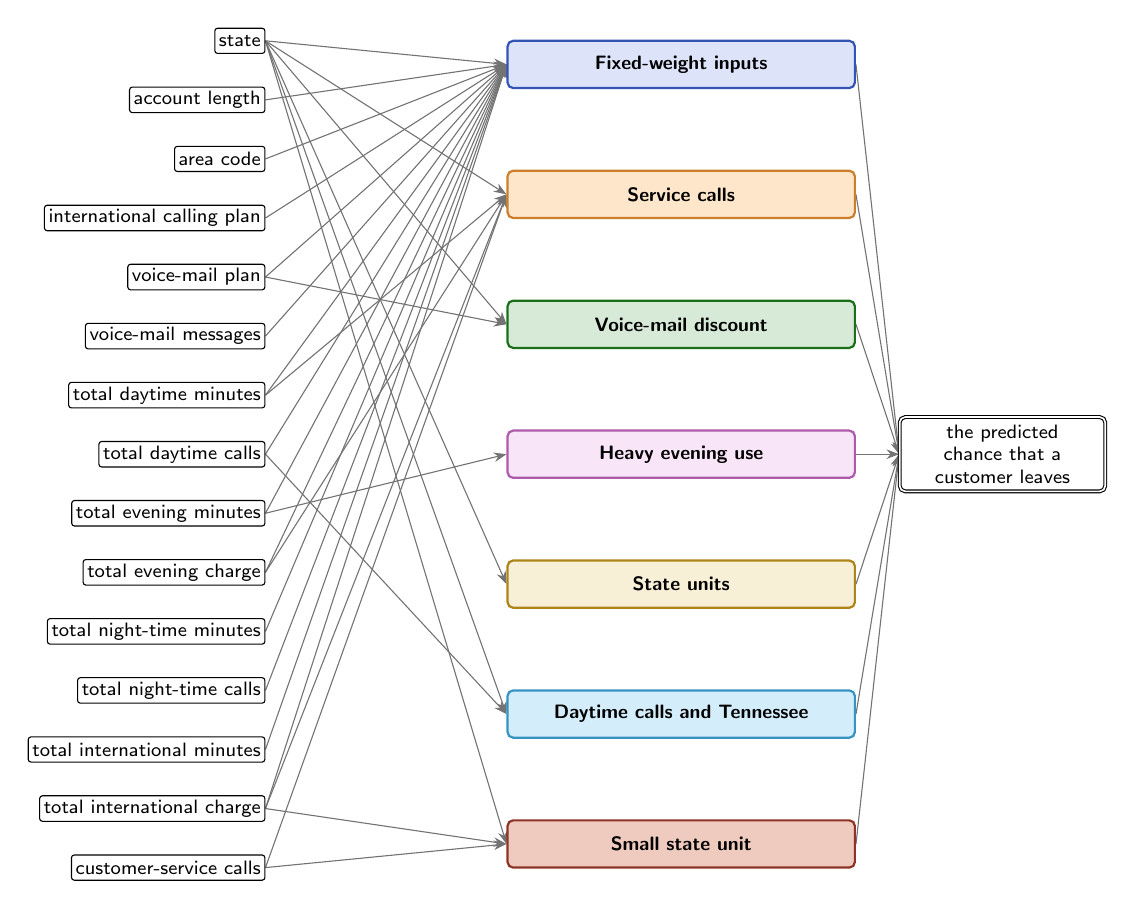
\begin{tikzpicture}[
  font=\sffamily\scriptsize, >={Stealth[length=1.6mm]},
  inp/.style={draw, rounded corners=1pt, fill=white, inner sep=1.5pt, minimum height=3.2mm, anchor=east},
  abox/.style={draw, thick, rounded corners=2pt, align=center, inner sep=3pt, minimum height=6mm, text width=42mm},
  outp/.style={draw, double, rounded corners=2pt, fill=white, align=center, inner sep=3pt, text width=24mm},
  agg/.style={draw=black!55},
]
\node[inp] (i0) at (0,5.25) {state};
\node[inp] (i1) at (0,4.5) {account length};
\node[inp] (i2) at (0,3.75) {area code};
\node[inp] (i3) at (0,3.0) {international calling plan};
\node[inp] (i4) at (0,2.25) {voice-mail plan};
\node[inp] (i5) at (0,1.5) {voice-mail messages};
\node[inp] (i6) at (0,0.75) {total daytime minutes};
\node[inp] (i7) at (0,-0.0) {total daytime calls};
\node[inp] (i8) at (0,-0.75) {total evening minutes};
\node[inp] (i9) at (0,-1.5) {total evening charge};
\node[inp] (i10) at (0,-2.25) {total night-time minutes};
\node[inp] (i11) at (0,-3.0) {total night-time calls};
\node[inp] (i12) at (0,-3.75) {total international minutes};
\node[inp] (i13) at (0,-4.5) {total international charge};
\node[inp] (i14) at (0,-5.25) {customer-service calls};
\node[abox, fill=RoyalBlue!18, draw=RoyalBlue!80!black] (b0) at (5.28,4.95) {\textbf{Fixed-weight inputs}};
\node[abox, fill=BurntOrange!18, draw=BurntOrange!80!black] (b1) at (5.28,3.3) {\textbf{Service calls}};
\node[abox, fill=ForestGreen!18, draw=ForestGreen!80!black] (b2) at (5.28,1.65) {\textbf{Voice-mail discount}};
\node[abox, fill=Orchid!18, draw=Orchid!80!black] (b3) at (5.28,0.0) {\textbf{Heavy evening use}};
\node[abox, fill=Goldenrod!18, draw=Goldenrod!80!black] (b4) at (5.28,-1.65) {\textbf{State units}};
\node[abox, fill=Cerulean!18, draw=Cerulean!80!black] (b5) at (5.28,-3.3) {\textbf{Daytime calls and Tennessee}};
\node[abox, fill=Mahogany!18, draw=Mahogany!80!black] (b6) at (5.28,-4.95) {\textbf{Small state unit}};
\node[outp] (out) at (9.36,0) {the predicted chance that a customer leaves};
\begin{scope}[on background layer]
\draw[->, agg, thin] (i0.east) -- (b0.west);
\draw[->, agg, thin] (i1.east) -- (b0.west);
\draw[->, agg, thin] (i2.east) -- (b0.west);
\draw[->, agg, thin] (i3.east) -- (b0.west);
\draw[->, agg, thin] (i4.east) -- (b0.west);
\draw[->, agg, thin] (i5.east) -- (b0.west);
\draw[->, agg, thin] (i6.east) -- (b0.west);
\draw[->, agg, thin] (i7.east) -- (b0.west);
\draw[->, agg, thin] (i8.east) -- (b0.west);
\draw[->, agg, thin] (i9.east) -- (b0.west);
\draw[->, agg, thin] (i10.east) -- (b0.west);
\draw[->, agg, thin] (i11.east) -- (b0.west);
\draw[->, agg, thin] (i12.east) -- (b0.west);
\draw[->, agg, thin] (i13.east) -- (b0.west);
\draw[->, agg] (b0.east) -- (out.west);
\draw[->, agg, thin] (i0.east) -- (b1.west);
\draw[->, agg, thin] (i6.east) -- (b1.west);
\draw[->, agg, thin] (i9.east) -- (b1.west);
\draw[->, agg, thin] (i13.east) -- (b1.west);
\draw[->, agg, thin] (i14.east) -- (b1.west);
\draw[->, agg] (b1.east) -- (out.west);
\draw[->, agg, thin] (i0.east) -- (b2.west);
\draw[->, agg, thin] (i4.east) -- (b2.west);
\draw[->, agg] (b2.east) -- (out.west);
\draw[->, agg, thin] (i8.east) -- (b3.west);
\draw[->, agg] (b3.east) -- (out.west);
\draw[->, agg, thin] (i0.east) -- (b4.west);
\draw[->, agg] (b4.east) -- (out.west);
\draw[->, agg, thin] (i0.east) -- (b5.west);
\draw[->, agg, thin] (i7.east) -- (b5.west);
\draw[->, agg] (b5.east) -- (out.west);
\draw[->, agg, thin] (i0.east) -- (b6.west);
\draw[->, agg, thin] (i13.east) -- (b6.west);
\draw[->, agg, thin] (i14.east) -- (b6.west);
\draw[->, agg] (b6.east) -- (out.west);
\end{scope}
\end{tikzpicture}}}%
\caption{The model at the level of the summary: one box per part.}
\label{fig:churn100s2c1:summary}
\end{figure}
\paragraph{Fixed-weight inputs.} This part adds up most inputs with fixed weights, and daytime minutes count most: they raise a typical customer's chance of leaving steadily, from under 1\% at 112 to about 13\% at 249 minutes.\,{\scriptsize\textcolor{NavyBlue}{[C057]}} An international plan takes the chance from about 1\% to about 13\%, a voice-mail plan lowers it to under 1\%, and more voice-mail messages raise it steadily, from about 1\% at 0 to about 5\% at 32 messages.\,{\scriptsize\textcolor{NavyBlue}{[C058, C067, C059]}} A higher international charge, more evening minutes, a higher evening charge and more night-time minutes also raise it steadily, each by one to two points.\,{\scriptsize\textcolor{NavyBlue}{[C062, C063, C064, C070]}} Through it, the state moves the chance from about 1\% in West Virginia to about 4\% in California and in Washington, and to under 1\% in Hawaii, Vermont and Colorado (41 to 80 training customers per state).\,{\scriptsize\textcolor{NavyBlue}{[C060, C061, C066, C068, C071]}}
\paragraph{Service calls.} This part adds up two parts: customer-service calls combined with low daytime use, and a rise from 4 calls upwards.\,{\scriptsize\textcolor{NavyBlue}{[C111]}} Through it, daytime minutes lower the chance only while they stay below about 170 minutes (between 147 and 216 minutes for different customers), in an uneven way: for a typical customer, from about 38\% at 91 minutes to about 1\% at 352 minutes.\,{\scriptsize\textcolor{NavyBlue}{[C107]}} With an evening charge above 17.12 US dollars, the chance is lowest at about 154 minutes of daytime use and higher either side: from about 1\% at 112 minutes to about 17\% at 249 minutes, against about 2\% to about 10\% at or below that charge.\,{\scriptsize\textcolor{NavyBlue}{[C103]}} Customer-service calls add to it from 4 calls upwards, in an uneven way: for a typical such customer, from about 3\% at 0 calls to about 11\% at 4 calls.\,{\scriptsize\textcolor{NavyBlue}{[C108]}}
\paragraph{Voice-mail discount.} This part reads the voice-mail plan and a few states: through it, a voice-mail plan lowers a typical customer's chance by less than a point, and customers in states other than Alabama, North Carolina and West Virginia get about 2\% instead of about 1\%.\,{\scriptsize\textcolor{NavyBlue}{[C125, C126]}}
\paragraph{Heavy evening use.} Through this part, evening minutes add nothing until about 239 minutes, then lower the chance steadily; it acts on 885 of 4000 training customers, 165 of whom left, and for the typical customer it acts on, the chance is about 5\% without it and about 4\% with it.\,{\scriptsize\textcolor{NavyBlue}{[C135, C136]}}
\paragraph{State units.} This part reads only the state and moves the chance by less than half a point: up in Arizona and Ohio, down in Nevada.\,{\scriptsize\textcolor{NavyBlue}{[C138, C139, C140]}}
\paragraph{Daytime calls and Tennessee.} This part reads the state and daytime calls: being in Tennessee raises a typical customer's chance from about 1\% to about 2\%, and daytime calls barely change it.\,{\scriptsize\textcolor{NavyBlue}{[C144, C145]}}
\paragraph{Small state unit.} This small part moves the chance by less than a tenth of a point, up in Arkansas and Utah.\,{\scriptsize\textcolor{NavyBlue}{[C150, C153]}}
\paragraph{The whole network.} Figure~\ref{fig:churn100s2c1:overview} (next page, landscape) draws every unit and connection of the explained model, nested by part: shaded clusters are the parts of the model and darker boxes the parts inside them; circles are hidden units (h1, h2, \ldots); each cluster's rectangle is its output, and a dashed `sum' stands for an addition the next unit does (drawn, not a unit of the model); the hexagon is the model's output. An input used by several parts is drawn under each of them (same label, dotted outline, the first copy marked with the number of copies): it is the same input, repeated for readability. Not used by the model (input columns with no connection): state: 20 of 51 levels, total daytime charge, total evening calls, total night-time charge, total international calls.
\begin{landscape}
\begin{figure}[p]\centering
\resizebox{\linewidth}{!}{%
\definecolor{netup}{HTML}{D95F02}\definecolor{netdown}{HTML}{1B9E77}\definecolor{netmixed}{HTML}{7F7F7F}%
\begin{tikzpicture}[
  font=\sffamily\scriptsize, >={Stealth[length=1.4mm]},
  inp/.style={draw, circle, fill=white, minimum size=3.2mm, inner sep=0pt},
  hid/.style={draw, circle, fill=white, minimum size=5.2mm, inner sep=0.5pt, font=\sffamily\tiny},
  exitbox/.style={draw, thick, rectangle, fill=white, align=center, text width=17mm, minimum height=5mm, inner sep=1.5pt, font=\sffamily\tiny},
  sumbox/.style={draw, thick, dashed, rectangle, fill=white, align=center, text width=17mm, minimum height=5mm, inner sep=1.5pt, font=\sffamily\tiny},
  outp/.style={draw, thick, regular polygon, regular polygon sides=6, fill=white, minimum size=10mm, inner sep=0pt, font=\sffamily\tiny, align=center},
  stub/.style={draw, dashed, rounded corners=2pt, fill=white, align=center, inner sep=2pt, font=\sffamily\tiny, text width=15mm},
  inlab/.style={font=\sffamily\tiny, align=center, text width=15mm, inner sep=1pt, fill=white, fill opacity=0.8, text opacity=1},
  wpos/.style={draw=NavyBlue}, wneg/.style={draw=BrickRed}, wagg/.style={draw=black!45, line width=1.2pt},
  wmix/.style={draw=Plum},
]
\node[outp] (n0) at (27.65,8.85) {churn};
\node[hid] (n10249) at (35.07,1.9) {h14};
\node[hid] (n1133) at (26.34,3.25) {h5};
\node[exitbox] (n11427) at (45.66,1.9) {Daytime calls and Tennessee $\uparrow$};
\node[hid] (n11951) at (36.57,1.9) {h16};
\node[hid] (n1264) at (14.74,5.95) {h6};
\node[hid] (n12926) at (13.99,1.9) {h17};
\node[hid] (n13827) at (38.07,4.6) {h18};
\node[hid] (n14942) at (38.07,1.9) {h19};
\node[hid] (n161) at (51.85,1.9) {h1};
\node[hid] (n17032) at (18.57,1.9) {h20};
\node[exitbox] (n252) at (52.6,4.6) {Small state unit $\uparrow$};
\node[hid] (n2627xa) at (52.6,3.25) {h21};
\node[hid] (n2627xb) at (13.99,3.25) {h22};
\node[hid] (n2796) at (15.49,3.25) {h7};
\node[hid] (n3861) at (39.57,1.9) {h8};
\node[hid] (n4051) at (26.34,4.6) {h9};
\node[exitbox] (n476) at (31.48,1.9) {Heavy evening use $\downarrow$};
\node[hid] (n5577) at (26.34,1.9) {h10};
\node[hid] (n6730) at (38.07,3.25) {h11};
\node[hid] (n7208) at (18.57,3.25) {h12};
\node[hid] (n807) at (14.74,4.6) {h4};
\node[hid] (n8896) at (41.07,1.9) {h13};
\node[hid] (n9555xa) at (53.35,1.9) {h23};
\node[hid] (n9555xb) at (15.49,1.9) {h24};
\node[exitbox] (nidentityxlin) at (5.85,1.9) {Fixed-weight inputs $\uparrow$};
\node[exitbox] (nidentityxsvc) at (21.9,7.3) {Service calls $\uparrow$};
\node[sumbox] (ncsumxxannx95) at (26.34,5.95) {sum: Voice-mail discount $\downarrow$};
\node[sumbox] (ncsumxxannx96) at (38.07,5.95) {sum: State units $\updownarrow$};
\node[inp, densely dotted, thick, draw=netmixed, very thick] (ngrpxxstatexxannx92) at (50.8,0.0) {};
\path (ngrpxxstatexxannx92.south) node[inlab, anchor=north] (labngrpxxstatexxannx92) {state (31 of 51 used) ($\times$6) $\updownarrow$};
\node[inp, densely dotted, thick, draw=netmixed, very thick] (ngrpxxstatexxannx95) at (27.24,0.0) {};
\path (ngrpxxstatexxannx95.south) node[inlab, anchor=north] (labngrpxxstatexxannx95) {state (31 of 51 used) $\updownarrow$};
\node[inp, densely dotted, thick, draw=netmixed, very thick] (ngrpxxstatexxannx96) at (38.07,0.0) {};
\path (ngrpxxstatexxannx96.south) node[inlab, anchor=north] (labngrpxxstatexxannx96) {state (31 of 51 used) $\updownarrow$};
\node[inp, densely dotted, thick, draw=netmixed, very thick] (ngrpxxstatexxannx97) at (44.76,0.0) {};
\path (ngrpxxstatexxannx97.south) node[inlab, anchor=north] (labngrpxxstatexxannx97) {state (31 of 51 used) $\updownarrow$};
\node[inp, densely dotted, thick, draw=netup, very thick] (ninxxnumberxcustomerxservicexcallsxxannx101) at (18.07,0.0) {};
\path (ninxxnumberxcustomerxservicexcallsxxannx101.south) node[inlab, anchor=north] (labninxxnumberxcustomerxservicexcallsxxannx101) {customer-service calls ($\times$2) $\uparrow$};
\node[inp, densely dotted, thick, draw=netdown, very thick] (ninxxtotalxintlxchargexxannx92) at (52.6,0.0) {};
\path (ninxxtotalxintlxchargexxannx92.south) node[inlab, anchor=north] (labninxxtotalxintlxchargexxannx92) {total international charge ($\times$3) $\downarrow$};
\node[inp, densely dotted, thick, draw=netdown, very thick] (ninxxtotalxintlxchargexxannx101) at (16.27,0.0) {};
\path (ninxxtotalxintlxchargexxannx101.south) node[inlab, anchor=north] (labninxxtotalxintlxchargexxannx101) {total international charge $\downarrow$};
\node[inp, densely dotted, thick, draw=netdown, very thick] (ninxxtotalxevexchargexxannx101) at (19.87,0.0) {};
\path (ninxxtotalxevexchargexxannx101.south) node[inlab, anchor=north] (labninxxtotalxevexchargexxannx101) {total evening charge ($\times$2) $\downarrow$};
\node[inp, densely dotted, thick, draw=netdown, very thick] (ninxxtotalxevexminutesxxannx94) at (31.48,0.0) {};
\path (ninxxtotalxevexminutesxxannx94.south) node[inlab, anchor=north] (labninxxtotalxevexminutesxxannx94) {total evening minutes ($\times$2) $\downarrow$};
\node[inp, densely dotted, thick, draw=netdown, very thick] (ninxxtotalxdayxcallsxxannx97) at (46.56,0.0) {};
\path (ninxxtotalxdayxcallsxxannx97.south) node[inlab, anchor=north] (labninxxtotalxdayxcallsxxannx97) {total daytime calls ($\times$2) $\downarrow$};
\node[inp, densely dotted, thick, draw=netdown, very thick] (ninxxtotalxdayxminutesxxannx101) at (14.47,0.0) {};
\path (ninxxtotalxdayxminutesxxannx101.south) node[inlab, anchor=north] (labninxxtotalxdayxminutesxxannx101) {total daytime minutes ($\times$2) $\downarrow$};
\node[inp, densely dotted, thick, draw=netdown, very thick] (ninxxvoicexmailxplanxxannx95) at (25.44,0.0) {};
\path (ninxxvoicexmailxplanxxannx95.south) node[inlab, anchor=north] (labninxxvoicexmailxplanxxannx95) {a voice-mail plan ($\times$2) $\downarrow$};
\node[inp, densely dotted, thick, draw=netmixed, very thick] (ngrpxxstatexxannx101) at (21.67,0.0) {};
\path (ngrpxxstatexxannx101.south) node[inlab, anchor=north] (labngrpxxstatexxannx101) {state (31 of 51 used) $\updownarrow$};
\node[inp, densely dotted, thick, draw=netdown, very thick] (ninxxnumberxcustomerxservicexcallsxxannx92) at (54.4,0.0) {};
\path (ninxxnumberxcustomerxservicexcallsxxannx92.south) node[inlab, anchor=north] (labninxxnumberxcustomerxservicexcallsxxannx92) {customer-service calls $\downarrow$};
\node[inp, densely dotted, thick, draw=netmixed, very thick] (ngrpxxstatexxannx99) at (4.5,0.0) {};
\path (ngrpxxstatexxannx99.south) node[inlab, anchor=north] (labngrpxxstatexxannx99) {state (31 of 51 used) $\updownarrow$};
\node[inp, draw=netup, very thick] (ninxxaccountxlengthxxannx99) at (0.9,-2.1) {};
\path (ninxxaccountxlengthxxannx99.south) node[inlab, anchor=north] (labninxxaccountxlengthxxannx99) {account length $\uparrow$};
\node[inp, draw=netdown, very thick] (ninxxareaxcodex408xxannx99) at (2.7,0.0) {};
\path (ninxxareaxcodex408xxannx99.south) node[inlab, anchor=north] (labninxxareaxcodex408xxannx99) {area code 408 $\downarrow$};
\node[inp, draw=netup, very thick] (ninxxareaxcodex415xxannx99) at (2.7,-2.1) {};
\path (ninxxareaxcodex415xxannx99.south) node[inlab, anchor=north] (labninxxareaxcodex415xxannx99) {area code 415 $\uparrow$};
\node[inp, draw=netdown, very thick] (ninxxareaxcodex510xxannx99) at (3.6,-1.05) {};
\path (ninxxareaxcodex510xxannx99.south) node[inlab, anchor=north] (labninxxareaxcodex510xxannx99) {area code 510 $\downarrow$};
\node[inp, draw=netup, very thick] (ninxxinternationalxplanxxannx99) at (1.8,-1.05) {};
\path (ninxxinternationalxplanxxannx99.south) node[inlab, anchor=north] (labninxxinternationalxplanxxannx99) {an international plan $\uparrow$};
\node[inp, draw=netup, very thick] (ninxxnumberxvmailxmessagesxxannx99) at (10.8,-1.05) {};
\path (ninxxnumberxvmailxmessagesxxannx99.south) node[inlab, anchor=north] (labninxxnumberxvmailxmessagesxxannx99) {voice-mail messages $\uparrow$};
\node[inp, draw=netup, very thick] (ninxxtotalxnightxminutesxxannx99) at (9.9,0.0) {};
\path (ninxxtotalxnightxminutesxxannx99.south) node[inlab, anchor=north] (labninxxtotalxnightxminutesxxannx99) {total night-time minutes $\uparrow$};
\node[inp, draw=netdown, very thick] (ninxxtotalxnightxcallsxxannx99) at (9.0,-1.05) {};
\path (ninxxtotalxnightxcallsxxannx99.south) node[inlab, anchor=north] (labninxxtotalxnightxcallsxxannx99) {total night-time calls $\downarrow$};
\node[inp, draw=netdown, very thick] (ninxxtotalxintlxminutesxxannx99) at (8.1,0.0) {};
\path (ninxxtotalxintlxminutesxxannx99.south) node[inlab, anchor=north] (labninxxtotalxintlxminutesxxannx99) {total international minutes $\downarrow$};
\node[inp, densely dotted, thick, draw=netup, very thick] (ninxxtotalxintlxchargexxannx99) at (7.2,-1.05) {};
\path (ninxxtotalxintlxchargexxannx99.south) node[inlab, anchor=north] (labninxxtotalxintlxchargexxannx99) {total international charge $\uparrow$};
\node[inp, densely dotted, thick, draw=netup, very thick] (ninxxtotalxevexchargexxannx99) at (6.3,0.0) {};
\path (ninxxtotalxevexchargexxannx99.south) node[inlab, anchor=north] (labninxxtotalxevexchargexxannx99) {total evening charge $\uparrow$};
\node[inp, densely dotted, thick, draw=netup, very thick] (ninxxtotalxevexminutesxxannx99) at (6.3,-2.1) {};
\path (ninxxtotalxevexminutesxxannx99.south) node[inlab, anchor=north] (labninxxtotalxevexminutesxxannx99) {total evening minutes $\uparrow$};
\node[inp, densely dotted, thick, draw=netup, very thick] (ninxxtotalxdayxcallsxxannx99) at (4.5,-2.1) {};
\path (ninxxtotalxdayxcallsxxannx99.south) node[inlab, anchor=north] (labninxxtotalxdayxcallsxxannx99) {total daytime calls $\uparrow$};
\node[inp, densely dotted, thick, draw=netup, very thick] (ninxxtotalxdayxminutesxxannx99) at (5.4,-1.05) {};
\path (ninxxtotalxdayxminutesxxannx99.south) node[inlab, anchor=north] (labninxxtotalxdayxminutesxxannx99) {total daytime minutes $\uparrow$};
\node[inp, densely dotted, thick, draw=netdown, very thick] (ninxxvoicexmailxplanxxannx99) at (0.9,0.0) {};
\path (ninxxvoicexmailxplanxxannx99.south) node[inlab, anchor=north] (labninxxvoicexmailxplanxxannx99) {a voice-mail plan $\downarrow$};
\node[font=\sffamily\tiny\bfseries, text=ForestGreen!60!black, inner sep=1pt] (subt0) at (14.74,6.45) {Calls with low usage};
\node[font=\sffamily\tiny\bfseries, text=ForestGreen!60!black, inner sep=1pt] (subt1) at (18.57,3.75) {Many service calls};
\begin{scope}[on background layer]
\node[fit=(nidentityxlin) , inner sep=8pt, rounded corners=5pt, fill=BurntOrange!10, draw=BurntOrange!45] (clu1) {};
\node[fit=(n1264) (n12926) (n17032) (n2627xb) (n2796) (n7208) (n807) (n9555xb) (nidentityxsvc) (subt0) (subt1), inner sep=8pt, rounded corners=5pt, fill=ForestGreen!10, draw=ForestGreen!45] (clu2) {};
\node[fit=(n1133) (n4051) (n5577) (ncsumxxannx95) , inner sep=8pt, rounded corners=5pt, fill=Orchid!10, draw=Orchid!45] (clu3) {};
\node[fit=(n476) , inner sep=8pt, rounded corners=5pt, fill=Goldenrod!10, draw=Goldenrod!45] (clu4) {};
\node[fit=(n10249) (n11951) (n13827) (n14942) (n3861) (n6730) (n8896) (ncsumxxannx96) , inner sep=8pt, rounded corners=5pt, fill=Cerulean!10, draw=Cerulean!45] (clu5) {};
\node[fit=(n11427) , inner sep=8pt, rounded corners=5pt, fill=Mahogany!10, draw=Mahogany!45] (clu6) {};
\node[fit=(n161) (n252) (n2627xa) (n9555xa) , inner sep=8pt, rounded corners=5pt, fill=OliveGreen!10, draw=OliveGreen!45] (clu7) {};
\node[fit=(n1264) (n12926) (n2627xb) (n2796) (n807) (n9555xb) (subt0), inner sep=4pt, rounded corners=3pt, fill=ForestGreen!26, draw=ForestGreen!70] {};
\node[fit=(n17032) (n7208) (subt1), inner sep=4pt, rounded corners=3pt, fill=ForestGreen!26, draw=ForestGreen!70] {};
\draw[->, wpos, line width=0.26pt] (n252) -- (n0);
\draw[->, wneg, line width=0.44pt] (n476) -- (n0);
\draw[->, wneg, line width=0.58pt] (n1133) -- (ncsumxxannx95);
\draw[->, wneg, line width=0.30pt] (n3861) -- (ncsumxxannx96);
\draw[->, wneg, line width=0.60pt] (n4051) -- (ncsumxxannx95);
\draw[->, wpos, line width=0.26pt] (n8896) -- (ncsumxxannx96);
\draw[->, wpos, line width=0.26pt] (n10249) -- (ncsumxxannx96);
\draw[->, wpos, line width=0.27pt] (n11427) -- (n0);
\draw[->, wpos, line width=0.40pt] (n13827) -- (ncsumxxannx96);
\draw[->, wpos, line width=0.26pt] (n14942) -- (ncsumxxannx96);
\draw[->, wpos, line width=0.53pt] (n161) -- (n252);
\draw[->, wpos, line width=0.47pt] (n2796) -- (n807);
\draw[->, wpos, line width=0.38pt] (n807) -- (n1264);
\draw[->, wpos, line width=0.65pt] (n1133) -- (n4051);
\draw[->, wpos, line width=0.30pt] (n5577) -- (n1133);
\draw[->, wneg, line width=0.25pt] (n11951) -- (n6730);
\draw[->, wpos, line width=0.37pt] (n12926) -- (n2796);
\draw[->, wpos, line width=0.44pt] (n17032) -- (n7208);
\draw[->, wpos, line width=0.60pt] (n6730) -- (n13827);
\draw[->, wneg, line width=0.38pt] (n2627xa) -- (n252);
\draw[->, wpos, line width=0.49pt] (n2627xb) -- (n807);
\draw[->, wpos, line width=0.36pt] (n9555xa) -- (n2627xa);
\draw[->, wpos, line width=0.36pt] (n9555xb) -- (n2627xb);
\draw[->, wpos, line width=0.60pt] (ninxxnumberxcustomerxservicexcallsxxannx101) -- (n17032);
\draw[->, wneg, line width=0.55pt] (ninxxtotalxintlxchargexxannx92) -- (n252);
\draw[->, wneg, line width=0.36pt] (ninxxtotalxintlxchargexxannx101) -- (n1264);
\draw[->, wneg, line width=0.60pt] (ninxxtotalxevexchargexxannx101) -- (n2796);
\draw[->, wpos, line width=0.63pt] (ninxxtotalxevexminutesxxannx94) -- (n476);
\draw[->, wneg, line width=0.29pt] (ninxxtotalxdayxcallsxxannx97) -- (n11427);
\draw[->, wneg, line width=0.74pt] (ninxxtotalxdayxminutesxxannx101) -- (n807);
\draw[->, wpos, line width=0.60pt] (ninxxvoicexmailxplanxxannx95) -- (n5577);
\draw[->, wpos, line width=0.26pt] (ninxxnumberxcustomerxservicexcallsxxannx101) -- (n807);
\draw[->, wpos, line width=0.38pt] (ninxxnumberxcustomerxservicexcallsxxannx101) -- (n2796);
\draw[->, wpos, line width=0.60pt] (ninxxnumberxcustomerxservicexcallsxxannx101) -- (n12926);
\draw[->, wpos, line width=0.35pt] (ninxxnumberxcustomerxservicexcallsxxannx101) -- (n2627xb);
\draw[->, wpos, line width=0.55pt] (ninxxnumberxcustomerxservicexcallsxxannx101) -- (n9555xb);
\draw[->, wpos, line width=0.35pt] (ninxxnumberxcustomerxservicexcallsxxannx92) -- (n2627xa);
\draw[->, wpos, line width=0.55pt] (ninxxnumberxcustomerxservicexcallsxxannx92) -- (n9555xa);
\draw[->, wpos, line width=0.30pt] (ninxxaccountxlengthxxannx99) -- (nidentityxlin);
\draw[->, wneg, line width=0.26pt] (ninxxareaxcodex408xxannx99) -- (nidentityxlin);
\draw[->, wpos, line width=0.27pt] (ninxxareaxcodex415xxannx99) -- (nidentityxlin);
\draw[->, wneg, line width=0.26pt] (ninxxareaxcodex510xxannx99) -- (nidentityxlin);
\draw[->, wpos, line width=0.51pt] (ninxxinternationalxplanxxannx99) -- (nidentityxlin);
\draw[->, wpos, line width=0.47pt] (ninxxnumberxvmailxmessagesxxannx99) -- (nidentityxlin);
\draw[->, wpos, line width=0.36pt] (ninxxtotalxnightxminutesxxannx99) -- (nidentityxlin);
\draw[->, wneg, line width=0.25pt] (ninxxtotalxnightxcallsxxannx99) -- (nidentityxlin);
\draw[->, wneg, line width=0.26pt] (ninxxtotalxintlxminutesxxannx99) -- (nidentityxlin);
\draw[->, wpos, line width=0.50pt] (ninxxtotalxintlxchargexxannx99) -- (nidentityxlin);
\draw[->, wpos, line width=0.41pt] (ninxxtotalxevexchargexxannx99) -- (nidentityxlin);
\draw[->, wpos, line width=0.43pt] (ninxxtotalxevexminutesxxannx99) -- (nidentityxlin);
\draw[->, wpos, line width=0.29pt] (ninxxtotalxdayxcallsxxannx99) -- (nidentityxlin);
\draw[->, wpos, line width=0.96pt] (ninxxtotalxdayxminutesxxannx99) -- (nidentityxlin);
\draw[->, wneg, line width=0.56pt] (ninxxvoicexmailxplanxxannx99) -- (nidentityxlin);
\draw[->, wpos, line width=0.60pt] (nidentityxlin) -- (n0);
\draw[->, wpos, line width=0.81pt] (n807) -- (nidentityxsvc);
\draw[->, wpos, line width=0.88pt] (n1264) -- (nidentityxsvc);
\draw[->, wpos, line width=0.77pt] (n7208) -- (nidentityxsvc);
\draw[->, wpos, line width=0.60pt] (nidentityxsvc) -- (n0);
\draw[->, wagg] (ncsumxxannx95) -- (n0);
\draw[->, wagg] (ncsumxxannx96) -- (n0);
\draw[->, wneg, line width=0.25pt] (ngrpxxstatexxannx92) -- node[pos=0.8, sloped, above, font=\sffamily\tiny, inner sep=1pt, fill=white, fill opacity=0.8, text opacity=1] {-0.01} (n161);
\draw[->, wpos, line width=0.34pt] (ngrpxxstatexxannx95) -- node[pos=0.8, sloped, above, font=\sffamily\tiny, inner sep=1pt, fill=white, fill opacity=0.8, text opacity=1] {+0.26} (n5577);
\draw[->, wpos, line width=0.52pt] (ngrpxxstatexxannx92) -- node[pos=0.8, sloped, above, font=\sffamily\tiny, inner sep=1pt, fill=white, fill opacity=0.8, text opacity=1] {2 edges, +0.44 to +0.76} (n252);
\draw[->, wneg, line width=0.60pt] (ngrpxxstatexxannx96) -- node[pos=0.8, sloped, above, font=\sffamily\tiny, inner sep=1pt, fill=white, fill opacity=0.8, text opacity=1] {-1.00} (n8896);
\draw[->, wmix, line width=0.40pt] (ngrpxxstatexxannx96) -- node[pos=0.8, sloped, above, font=\sffamily\tiny, inner sep=1pt, fill=white, fill opacity=0.8, text opacity=1] {3 edges, -0.42 to +0.00} (n6730);
\draw[->, wpos, line width=0.60pt] (ngrpxxstatexxannx97) -- node[pos=0.8, sloped, above, font=\sffamily\tiny, inner sep=1pt, fill=white, fill opacity=0.8, text opacity=1] {+1.00} (n11427);
\draw[->, wneg, line width=0.52pt] (ngrpxxstatexxannx96) -- node[pos=0.8, sloped, above, font=\sffamily\tiny, inner sep=1pt, fill=white, fill opacity=0.8, text opacity=1] {-0.77} (n3861);
\draw[->, wpos, line width=0.27pt] (ngrpxxstatexxannx95) -- node[pos=0.8, sloped, above, font=\sffamily\tiny, inner sep=1pt, fill=white, fill opacity=0.8, text opacity=1] {+0.06} (n4051);
\draw[->, wneg, line width=0.38pt] (ngrpxxstatexxannx101) -- node[pos=0.8, sloped, above, font=\sffamily\tiny, inner sep=1pt, fill=white, fill opacity=0.8, text opacity=1] {-0.36} (n7208);
\draw[->, wpos, line width=0.30pt] (ngrpxxstatexxannx101) -- node[pos=0.8, sloped, above, font=\sffamily\tiny, inner sep=1pt, fill=white, fill opacity=0.8, text opacity=1] {+0.15} (n2796);
\draw[->, wpos, line width=0.60pt] (ngrpxxstatexxannx96) -- node[pos=0.8, sloped, above, font=\sffamily\tiny, inner sep=1pt, fill=white, fill opacity=0.8, text opacity=1] {+1.00} (n10249);
\draw[->, wpos, line width=0.26pt] (ngrpxxstatexxannx95) -- node[pos=0.8, sloped, above, font=\sffamily\tiny, inner sep=1pt, fill=white, fill opacity=0.8, text opacity=1] {+0.02} (n1133);
\draw[->, wpos, line width=0.60pt] (ngrpxxstatexxannx96) -- node[pos=0.8, sloped, above, font=\sffamily\tiny, inner sep=1pt, fill=white, fill opacity=0.8, text opacity=1] {+1.00} (n11951);
\draw[->, wpos, line width=0.60pt] (ngrpxxstatexxannx96) -- node[pos=0.8, sloped, above, font=\sffamily\tiny, inner sep=1pt, fill=white, fill opacity=0.8, text opacity=1] {+1.00} (n14942);
\draw[->, wmix, line width=0.36pt] (ngrpxxstatexxannx99) -- node[pos=0.8, sloped, above, font=\sffamily\tiny, inner sep=1pt, fill=white, fill opacity=0.8, text opacity=1] {25 edges, -0.30 to +0.15} (nidentityxlin);
\end{scope}
\node[font=\sffamily\scriptsize\bfseries, text=BurntOrange!55!black, anchor=south west, inner sep=1pt, fill=white, fill opacity=0.85, text opacity=1] at (clu1.north west) {Fixed-weight inputs};
\node[font=\sffamily\scriptsize\bfseries, text=ForestGreen!55!black, anchor=south west, inner sep=1pt, fill=white, fill opacity=0.85, text opacity=1] at (clu2.north west) {Service calls};
\node[font=\sffamily\scriptsize\bfseries, text=Orchid!55!black, anchor=south west, inner sep=1pt, fill=white, fill opacity=0.85, text opacity=1] at (clu3.north west) {Voice-mail discount};
\node[font=\sffamily\scriptsize\bfseries, text=Goldenrod!55!black, anchor=south west, inner sep=1pt, fill=white, fill opacity=0.85, text opacity=1] at (clu4.north west) {Heavy evening use};
\node[font=\sffamily\scriptsize\bfseries, text=Cerulean!55!black, anchor=south west, inner sep=1pt, fill=white, fill opacity=0.85, text opacity=1] at (clu5.north west) {State units};
\node[font=\sffamily\scriptsize\bfseries, text=Mahogany!55!black, anchor=south west, inner sep=1pt, fill=white, fill opacity=0.85, text opacity=1] at (clu6.north west) {Daytime calls and Tennessee};
\node[font=\sffamily\scriptsize\bfseries, text=OliveGreen!55!black, anchor=south west, inner sep=1pt, fill=white, fill opacity=0.85, text opacity=1] at (clu7.north west) {Small state unit};
\end{tikzpicture}}%
\caption{Every unit and connection of the explained model, nested by part. Blue: positive weight (raises the score); red: negative weight (lowers it); thicker: larger weight. Orange outline and up arrow: raises the final prediction; teal and down arrow: lowers it; grey and double arrow: depends.}
\label{fig:churn100s2c1:overview}
\end{figure}
\end{landscape}
\paragraph{Worth checking against what is known.} Worth checking: the state moves the chance by several points (for example California and Washington about 6\% and 5\%, Hawaii under 1\%), based on 41 to 122 training customers per state.\,{\scriptsize\textcolor{NavyBlue}{[C003, C004, C016]}} Worth checking: the model treats a voice-mail plan as lowering the chance of leaving but more voice-mail messages as raising it.\,{\scriptsize\textcolor{NavyBlue}{[C012, C005]}} Worth checking: the many-service-calls part is switched off for customers in West Virginia, the state of the typical customer.\,{\scriptsize\textcolor{NavyBlue}{[C130]}} Worth checking: daytime minutes, the evening charge and the international charge raise the chance through the fixed-weight inputs but lower it through calls with low usage.\,{\scriptsize\textcolor{NavyBlue}{[C057, C112, C064, C115, C062, C114]}}
\subsection{The model, read from the top down}
\noindent{\small Each part of the explanation in turn, from the whole model down to the smallest parts: what it does for the prediction (hypothesis), what was checked (evidence), a diagram one level down, and where to read on. The technical record of each part is in ``Technical detail'' at the end.\par}
\subsubsection{The whole model}\label{rd:ann102}
\noindent{\small Figure~\ref{fig:churn100s2c1:parts-ann102} shows what feeds this part; Figure~\ref{fig:churn100s2c1:units-ann102} its units and every connection into them (dashed boxes: connections from or to other parts, drawn in their own sections).\par}
\begin{figure}[H]\centering
\resizebox{!}{\ifdim\height>0.5\textheight 0.5\textheight\else\height\fi}{%
\resizebox{\ifdim\width>\linewidth\linewidth\else\width\fi}{!}{%
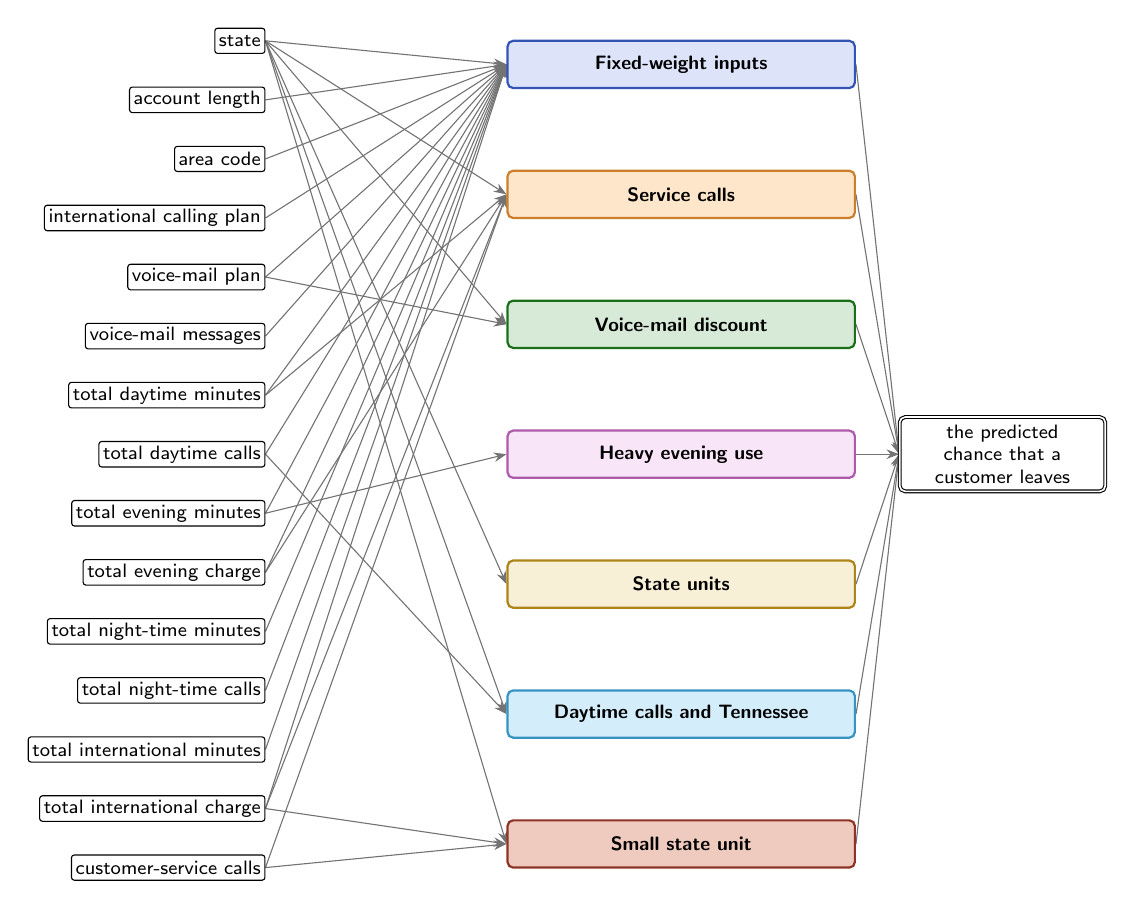
\begin{tikzpicture}[
  font=\sffamily\scriptsize, >={Stealth[length=1.6mm]},
  inp/.style={draw, rounded corners=1pt, fill=white, inner sep=1.5pt, minimum height=3.2mm, anchor=east},
  abox/.style={draw, thick, rounded corners=2pt, align=center, inner sep=3pt, minimum height=6mm, text width=42mm},
  outp/.style={draw, double, rounded corners=2pt, fill=white, align=center, inner sep=3pt, text width=24mm},
  agg/.style={draw=black!55},
]
\node[inp] (i0) at (0,5.25) {state};
\node[inp] (i1) at (0,4.5) {account length};
\node[inp] (i2) at (0,3.75) {area code};
\node[inp] (i3) at (0,3.0) {international calling plan};
\node[inp] (i4) at (0,2.25) {voice-mail plan};
\node[inp] (i5) at (0,1.5) {voice-mail messages};
\node[inp] (i6) at (0,0.75) {total daytime minutes};
\node[inp] (i7) at (0,-0.0) {total daytime calls};
\node[inp] (i8) at (0,-0.75) {total evening minutes};
\node[inp] (i9) at (0,-1.5) {total evening charge};
\node[inp] (i10) at (0,-2.25) {total night-time minutes};
\node[inp] (i11) at (0,-3.0) {total night-time calls};
\node[inp] (i12) at (0,-3.75) {total international minutes};
\node[inp] (i13) at (0,-4.5) {total international charge};
\node[inp] (i14) at (0,-5.25) {customer-service calls};
\node[abox, fill=RoyalBlue!18, draw=RoyalBlue!80!black] (b0) at (5.28,4.95) {\textbf{Fixed-weight inputs}};
\node[abox, fill=BurntOrange!18, draw=BurntOrange!80!black] (b1) at (5.28,3.3) {\textbf{Service calls}};
\node[abox, fill=ForestGreen!18, draw=ForestGreen!80!black] (b2) at (5.28,1.65) {\textbf{Voice-mail discount}};
\node[abox, fill=Orchid!18, draw=Orchid!80!black] (b3) at (5.28,0.0) {\textbf{Heavy evening use}};
\node[abox, fill=Goldenrod!18, draw=Goldenrod!80!black] (b4) at (5.28,-1.65) {\textbf{State units}};
\node[abox, fill=Cerulean!18, draw=Cerulean!80!black] (b5) at (5.28,-3.3) {\textbf{Daytime calls and Tennessee}};
\node[abox, fill=Mahogany!18, draw=Mahogany!80!black] (b6) at (5.28,-4.95) {\textbf{Small state unit}};
\node[outp] (out) at (9.36,0) {the predicted chance that a customer leaves};
\begin{scope}[on background layer]
\draw[->, agg, thin] (i0.east) -- (b0.west);
\draw[->, agg, thin] (i1.east) -- (b0.west);
\draw[->, agg, thin] (i2.east) -- (b0.west);
\draw[->, agg, thin] (i3.east) -- (b0.west);
\draw[->, agg, thin] (i4.east) -- (b0.west);
\draw[->, agg, thin] (i5.east) -- (b0.west);
\draw[->, agg, thin] (i6.east) -- (b0.west);
\draw[->, agg, thin] (i7.east) -- (b0.west);
\draw[->, agg, thin] (i8.east) -- (b0.west);
\draw[->, agg, thin] (i9.east) -- (b0.west);
\draw[->, agg, thin] (i10.east) -- (b0.west);
\draw[->, agg, thin] (i11.east) -- (b0.west);
\draw[->, agg, thin] (i12.east) -- (b0.west);
\draw[->, agg, thin] (i13.east) -- (b0.west);
\draw[->, agg] (b0.east) -- (out.west);
\draw[->, agg, thin] (i0.east) -- (b1.west);
\draw[->, agg, thin] (i6.east) -- (b1.west);
\draw[->, agg, thin] (i9.east) -- (b1.west);
\draw[->, agg, thin] (i13.east) -- (b1.west);
\draw[->, agg, thin] (i14.east) -- (b1.west);
\draw[->, agg] (b1.east) -- (out.west);
\draw[->, agg, thin] (i0.east) -- (b2.west);
\draw[->, agg, thin] (i4.east) -- (b2.west);
\draw[->, agg] (b2.east) -- (out.west);
\draw[->, agg, thin] (i8.east) -- (b3.west);
\draw[->, agg] (b3.east) -- (out.west);
\draw[->, agg, thin] (i0.east) -- (b4.west);
\draw[->, agg] (b4.east) -- (out.west);
\draw[->, agg, thin] (i0.east) -- (b5.west);
\draw[->, agg, thin] (i7.east) -- (b5.west);
\draw[->, agg] (b5.east) -- (out.west);
\draw[->, agg, thin] (i0.east) -- (b6.west);
\draw[->, agg, thin] (i13.east) -- (b6.west);
\draw[->, agg, thin] (i14.east) -- (b6.west);
\draw[->, agg] (b6.east) -- (out.west);
\end{scope}
\end{tikzpicture}}}%
\caption{The whole model: what feeds it, one level down.}
\label{fig:churn100s2c1:parts-ann102}
\end{figure}
\begin{figure}[H]\centering
\resizebox{\ifdim\width>\linewidth\linewidth\else\width\fi}{!}{%
\definecolor{netup}{HTML}{D95F02}\definecolor{netdown}{HTML}{1B9E77}\definecolor{netmixed}{HTML}{7F7F7F}%
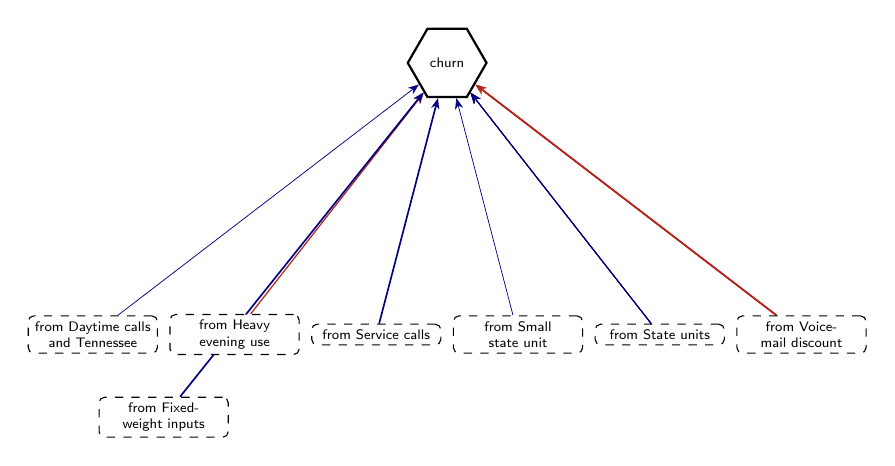
\begin{tikzpicture}[
  font=\sffamily\scriptsize, >={Stealth[length=1.4mm]},
  inp/.style={draw, circle, fill=white, minimum size=3.2mm, inner sep=0pt},
  hid/.style={draw, circle, fill=white, minimum size=5.2mm, inner sep=0.5pt, font=\sffamily\tiny},
  exitbox/.style={draw, thick, rectangle, fill=white, align=center, text width=17mm, minimum height=5mm, inner sep=1.5pt, font=\sffamily\tiny},
  sumbox/.style={draw, thick, dashed, rectangle, fill=white, align=center, text width=17mm, minimum height=5mm, inner sep=1.5pt, font=\sffamily\tiny},
  outp/.style={draw, thick, regular polygon, regular polygon sides=6, fill=white, minimum size=10mm, inner sep=0pt, font=\sffamily\tiny, align=center},
  stub/.style={draw, dashed, rounded corners=2pt, fill=white, align=center, inner sep=2pt, font=\sffamily\tiny, text width=15mm},
  inlab/.style={font=\sffamily\tiny, align=center, text width=15mm, inner sep=1pt, fill=white, fill opacity=0.8, text opacity=1},
  wpos/.style={draw=NavyBlue}, wneg/.style={draw=BrickRed}, wagg/.style={draw=black!45, line width=1.2pt},
  wmix/.style={draw=Plum},
]
\node[outp] (n0) at (5.4,3.45) {churn};
\node[stub] (nfromxxSmallxstatexunit) at (6.3,0.0) {from Small state unit};
\node[stub] (nfromxxHeavyxeveningxuse) at (2.7,0.0) {from Heavy evening use};
\node[stub] (nfromxxVoicemmailxdiscount) at (9.9,0.0) {from Voice-mail discount};
\node[stub] (nfromxxStatexunits) at (8.1,0.0) {from State units};
\node[stub] (nfromxxDaytimexcallsxandxTennessee) at (0.9,0.0) {from Daytime calls and Tennessee};
\node[stub] (nfromxxFixedmweightxinputs) at (1.8,-1.05) {from Fixed-weight inputs};
\node[stub] (nfromxxServicexcalls) at (4.5,0.0) {from Service calls};
\begin{scope}[on background layer]
\draw[->, wpos, line width=0.26pt] (nfromxxSmallxstatexunit) -- (n0);
\draw[->, wneg, line width=0.44pt] (nfromxxHeavyxeveningxuse) -- (n0);
\draw[->, wneg, line width=0.58pt] (nfromxxVoicemmailxdiscount) -- (n0);
\draw[->, wneg, line width=0.30pt] (nfromxxStatexunits) -- (n0);
\draw[->, wneg, line width=0.60pt] (nfromxxVoicemmailxdiscount) -- (n0);
\draw[->, wpos, line width=0.26pt] (nfromxxStatexunits) -- (n0);
\draw[->, wpos, line width=0.26pt] (nfromxxStatexunits) -- (n0);
\draw[->, wpos, line width=0.27pt] (nfromxxDaytimexcallsxandxTennessee) -- (n0);
\draw[->, wpos, line width=0.40pt] (nfromxxStatexunits) -- (n0);
\draw[->, wpos, line width=0.26pt] (nfromxxStatexunits) -- (n0);
\draw[->, wpos, line width=0.60pt] (nfromxxFixedmweightxinputs) -- (n0);
\draw[->, wpos, line width=0.60pt] (nfromxxServicexcalls) -- (n0);
\end{scope}
\end{tikzpicture}}%
\caption{The whole model: its units and every connection into them. Blue: positive weight (raises the score); red: negative weight (lowers it); thicker: larger weight. Orange outline and up arrow: raises the final prediction; teal and down arrow: lowers it; grey and double arrow: depends.}
\label{fig:churn100s2c1:units-ann102}
\end{figure}
\paragraph{Hypothesis.} The model adds up seven parts into one score: fixed-weight inputs, service calls, a voice-mail discount, heavy evening use, state units, a daytime-calls unit and a small state unit.\,{\scriptsize\textcolor{NavyBlue}{[C056]}}
\paragraph{Evidence.} It is made up of these seven parts (each explained below); the score is their sum, which was checked on all 4000 training customers.\,{\scriptsize\textcolor{NavyBlue}{[C056]}} Changing one input at a time across the whole model, an international plan takes a typical customer's chance of leaving from about 1\% to about 13\%, and a voice-mail plan lowers it to under 1\%.\,{\scriptsize\textcolor{NavyBlue}{[C001, C012]}} More customer-service calls raise it in an uneven way, from about 1\% at 0 calls to about 3\% at 3 calls.\,{\scriptsize\textcolor{NavyBlue}{[C008]}} The model ignores the daytime charge, evening calls, international calls and the night-time charge.\,{\scriptsize\textcolor{NavyBlue}{[C052, C053, C054, C055]}}
\par\noindent{\small Evidence plots: Figure~\ref{fig:churn100s2c1:plot-ann102-0}, Figure~\ref{fig:churn100s2c1:plot-ann102-1}.\par}
\begin{figure}[H]\centering
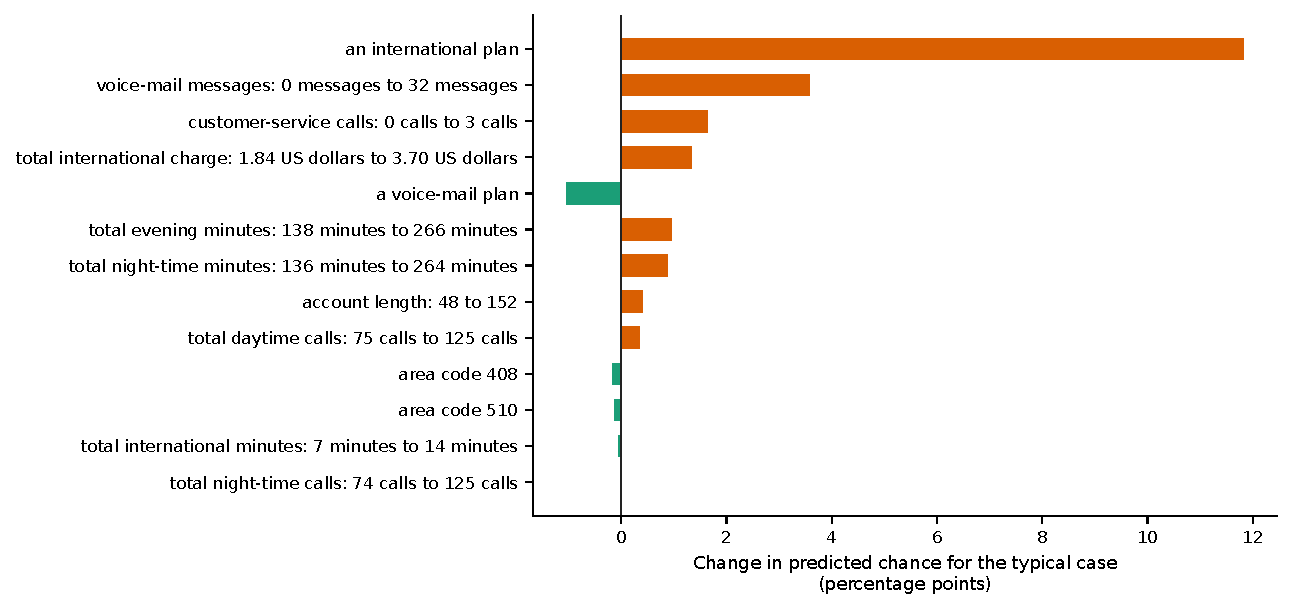
\includegraphics[width=\linewidth,height=0.88\textheight,keepaspectratio]{figures/churn100-s2-c1/ann_102-effects.pdf}
\caption{The whole model: Each input's change in the predicted value for the typical case across the whole model, largest first (orange: raises it, teal: lowers it).}
\label{fig:churn100s2c1:plot-ann102-0}
\end{figure}
\begin{figure}[H]\centering
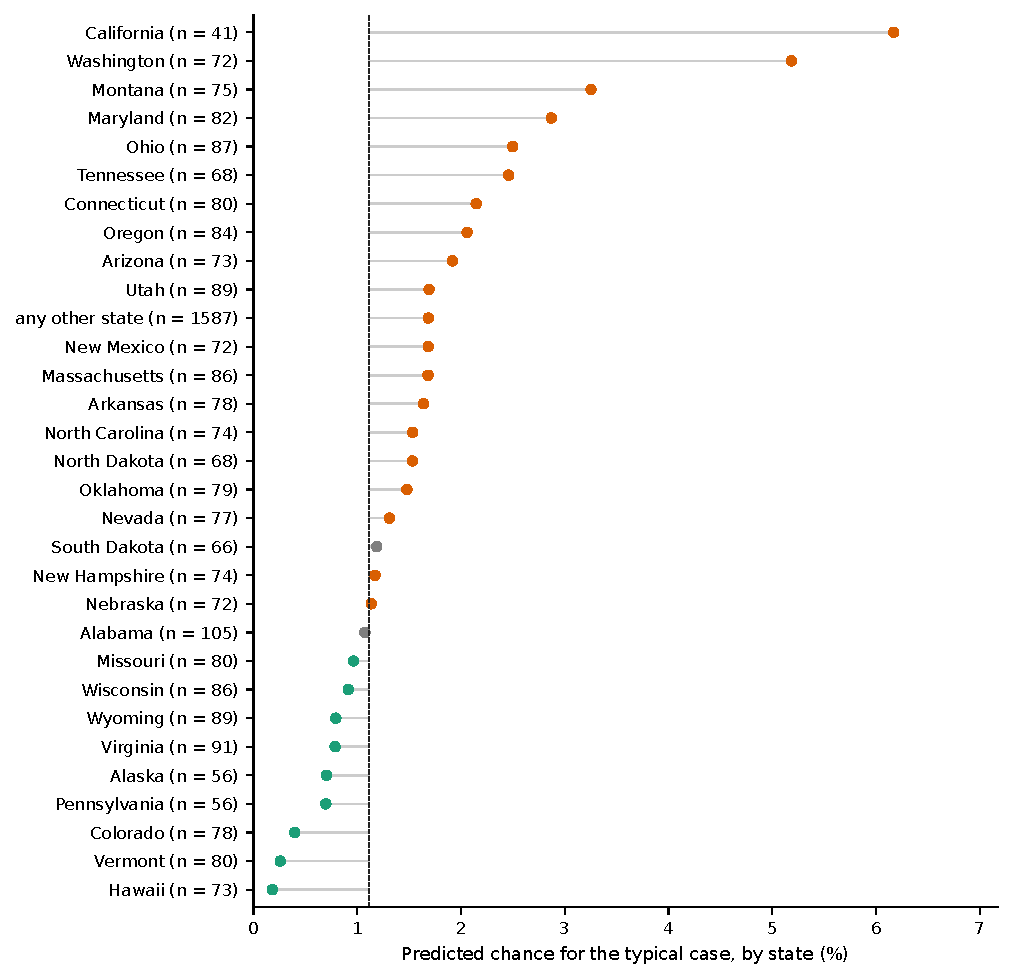
\includegraphics[width=\linewidth,height=0.88\textheight,keepaspectratio]{figures/churn100-s2-c1/ann_102-levels-state.pdf}
\caption{The whole model: Every level of state the model reads: the predicted value for the typical case at that level (dashed: the reference level); n = training customers; grey: few customers or not supported.}
\label{fig:churn100s2c1:plot-ann102-1}
\end{figure}
\par\smallskip\noindent{\small \textbf{Dive deeper:} Fixed-weight inputs (\ref{rd:ann99}); Service calls (\ref{rd:ann101}); Voice-mail discount (\ref{rd:ann95}); Heavy evening use (\ref{rd:ann94}); State units (\ref{rd:ann96}); Daytime calls and Tennessee (\ref{rd:ann97}); Small state unit (\ref{rd:ann92}). Technical detail: \ref{tech:ann102}.\par}
\subsubsection{Fixed-weight inputs}\label{rd:ann99}
\noindent{\footnotesize Part of: The whole model (\ref{rd:ann102}).\par}
\noindent{\small Figure~\ref{fig:churn100s2c1:parts-ann99} shows what feeds this part; Figure~\ref{fig:churn100s2c1:units-ann99} its units and every connection into them (dashed boxes: connections from or to other parts, drawn in their own sections).\par}
\begin{figure}[H]\centering
\resizebox{!}{\ifdim\height>0.5\textheight 0.5\textheight\else\height\fi}{%
\resizebox{\ifdim\width>\linewidth\linewidth\else\width\fi}{!}{%
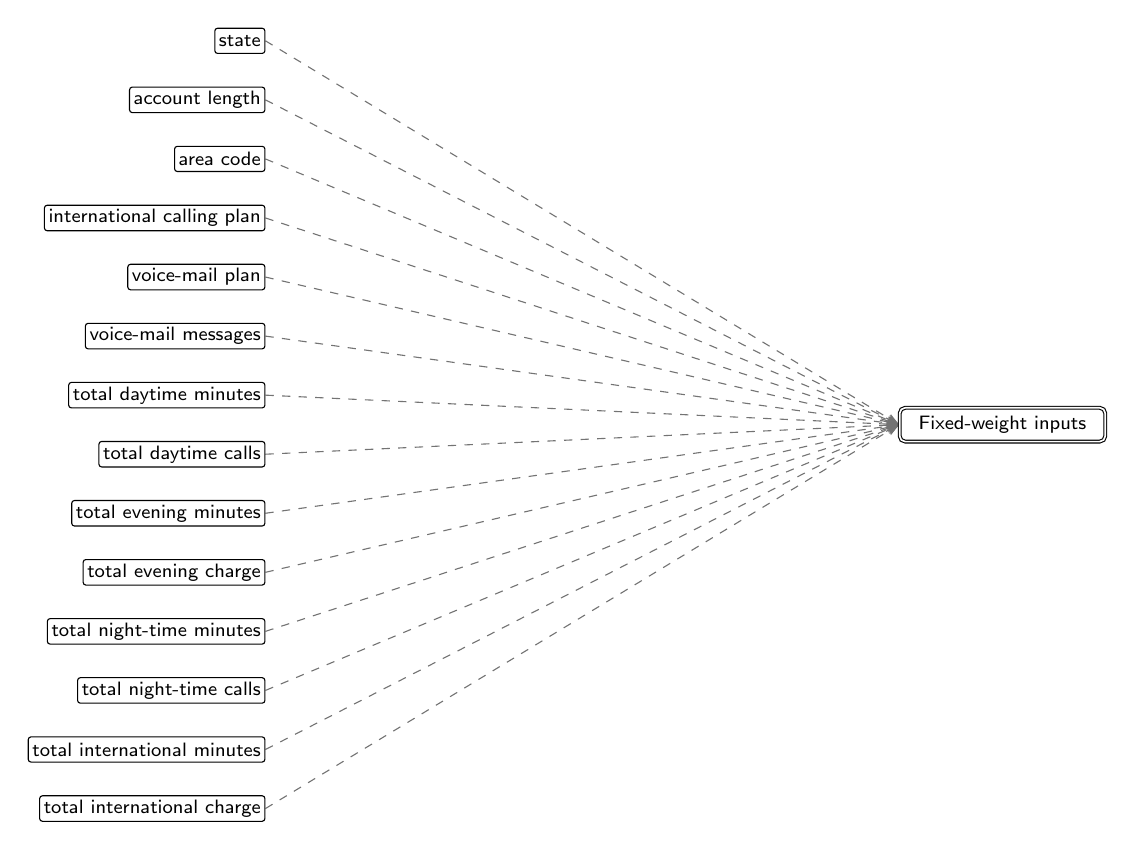
\begin{tikzpicture}[
  font=\sffamily\scriptsize, >={Stealth[length=1.6mm]},
  inp/.style={draw, rounded corners=1pt, fill=white, inner sep=1.5pt, minimum height=3.2mm, anchor=east},
  abox/.style={draw, thick, rounded corners=2pt, align=center, inner sep=3pt, minimum height=6mm, text width=42mm},
  outp/.style={draw, double, rounded corners=2pt, fill=white, align=center, inner sep=3pt, text width=24mm},
  agg/.style={draw=black!55},
]
\node[inp] (i0) at (0,4.875) {state};
\node[inp] (i1) at (0,4.125) {account length};
\node[inp] (i2) at (0,3.375) {area code};
\node[inp] (i3) at (0,2.625) {international calling plan};
\node[inp] (i4) at (0,1.875) {voice-mail plan};
\node[inp] (i5) at (0,1.125) {voice-mail messages};
\node[inp] (i6) at (0,0.375) {total daytime minutes};
\node[inp] (i7) at (0,-0.375) {total daytime calls};
\node[inp] (i8) at (0,-1.125) {total evening minutes};
\node[inp] (i9) at (0,-1.875) {total evening charge};
\node[inp] (i10) at (0,-2.625) {total night-time minutes};
\node[inp] (i11) at (0,-3.375) {total night-time calls};
\node[inp] (i12) at (0,-4.125) {total international minutes};
\node[inp] (i13) at (0,-4.875) {total international charge};
\node[outp] (out) at (9.36,0) {Fixed-weight inputs};
\begin{scope}[on background layer]
\draw[->, agg, thin, dashed] (i0.east) -- (out.west);
\draw[->, agg, thin, dashed] (i1.east) -- (out.west);
\draw[->, agg, thin, dashed] (i2.east) -- (out.west);
\draw[->, agg, thin, dashed] (i3.east) -- (out.west);
\draw[->, agg, thin, dashed] (i4.east) -- (out.west);
\draw[->, agg, thin, dashed] (i5.east) -- (out.west);
\draw[->, agg, thin, dashed] (i6.east) -- (out.west);
\draw[->, agg, thin, dashed] (i7.east) -- (out.west);
\draw[->, agg, thin, dashed] (i8.east) -- (out.west);
\draw[->, agg, thin, dashed] (i9.east) -- (out.west);
\draw[->, agg, thin, dashed] (i10.east) -- (out.west);
\draw[->, agg, thin, dashed] (i11.east) -- (out.west);
\draw[->, agg, thin, dashed] (i12.east) -- (out.west);
\draw[->, agg, thin, dashed] (i13.east) -- (out.west);
\end{scope}
\end{tikzpicture}}}%
\caption{Fixed-weight inputs: what feeds it, one level down.}
\label{fig:churn100s2c1:parts-ann99}
\end{figure}
\begin{figure}[H]\centering
\resizebox{\ifdim\width>\linewidth\linewidth\else\width\fi}{!}{%
\definecolor{netup}{HTML}{D95F02}\definecolor{netdown}{HTML}{1B9E77}\definecolor{netmixed}{HTML}{7F7F7F}%
\begin{tikzpicture}[
  font=\sffamily\scriptsize, >={Stealth[length=1.4mm]},
  inp/.style={draw, circle, fill=white, minimum size=3.2mm, inner sep=0pt},
  hid/.style={draw, circle, fill=white, minimum size=5.2mm, inner sep=0.5pt, font=\sffamily\tiny},
  exitbox/.style={draw, thick, rectangle, fill=white, align=center, text width=17mm, minimum height=5mm, inner sep=1.5pt, font=\sffamily\tiny},
  sumbox/.style={draw, thick, dashed, rectangle, fill=white, align=center, text width=17mm, minimum height=5mm, inner sep=1.5pt, font=\sffamily\tiny},
  outp/.style={draw, thick, regular polygon, regular polygon sides=6, fill=white, minimum size=10mm, inner sep=0pt, font=\sffamily\tiny, align=center},
  stub/.style={draw, dashed, rounded corners=2pt, fill=white, align=center, inner sep=2pt, font=\sffamily\tiny, text width=15mm},
  inlab/.style={font=\sffamily\tiny, align=center, text width=15mm, inner sep=1pt, fill=white, fill opacity=0.8, text opacity=1},
  wpos/.style={draw=NavyBlue}, wneg/.style={draw=BrickRed}, wagg/.style={draw=black!45, line width=1.2pt},
  wmix/.style={draw=Plum},
]
\node[exitbox] (nidentityxlin) at (5.85,1.9) {Fixed-weight inputs $\uparrow$};
\node[inp, draw=netmixed, very thick] (ngrpxxstate) at (4.5,0.0) {};
\path (ngrpxxstate.south) node[inlab, anchor=north] (labngrpxxstate) {state (31 of 51 used) $\updownarrow$};
\node[inp, draw=netup, very thick] (ninxxaccountxlength) at (0.9,-2.1) {};
\path (ninxxaccountxlength.south) node[inlab, anchor=north] (labninxxaccountxlength) {account length $\uparrow$};
\node[inp, draw=netdown, very thick] (ninxxareaxcodex408) at (2.7,0.0) {};
\path (ninxxareaxcodex408.south) node[inlab, anchor=north] (labninxxareaxcodex408) {area code 408 $\downarrow$};
\node[inp, draw=netup, very thick] (ninxxareaxcodex415) at (2.7,-2.1) {};
\path (ninxxareaxcodex415.south) node[inlab, anchor=north] (labninxxareaxcodex415) {area code 415 $\uparrow$};
\node[inp, draw=netdown, very thick] (ninxxareaxcodex510) at (3.6,-1.05) {};
\path (ninxxareaxcodex510.south) node[inlab, anchor=north] (labninxxareaxcodex510) {area code 510 $\downarrow$};
\node[inp, draw=netup, very thick] (ninxxinternationalxplan) at (1.8,-1.05) {};
\path (ninxxinternationalxplan.south) node[inlab, anchor=north] (labninxxinternationalxplan) {an international plan $\uparrow$};
\node[inp, draw=netup, very thick] (ninxxnumberxvmailxmessages) at (10.8,-1.05) {};
\path (ninxxnumberxvmailxmessages.south) node[inlab, anchor=north] (labninxxnumberxvmailxmessages) {voice-mail messages $\uparrow$};
\node[inp, draw=netup, very thick] (ninxxtotalxnightxminutes) at (9.9,0.0) {};
\path (ninxxtotalxnightxminutes.south) node[inlab, anchor=north] (labninxxtotalxnightxminutes) {total night-time minutes $\uparrow$};
\node[inp, draw=netdown, very thick] (ninxxtotalxnightxcalls) at (9.0,-1.05) {};
\path (ninxxtotalxnightxcalls.south) node[inlab, anchor=north] (labninxxtotalxnightxcalls) {total night-time calls $\downarrow$};
\node[inp, draw=netdown, very thick] (ninxxtotalxintlxminutes) at (8.1,0.0) {};
\path (ninxxtotalxintlxminutes.south) node[inlab, anchor=north] (labninxxtotalxintlxminutes) {total international minutes $\downarrow$};
\node[inp, draw=netup, very thick] (ninxxtotalxintlxcharge) at (7.2,-1.05) {};
\path (ninxxtotalxintlxcharge.south) node[inlab, anchor=north] (labninxxtotalxintlxcharge) {total international charge $\uparrow$};
\node[inp, draw=netup, very thick] (ninxxtotalxevexcharge) at (6.3,0.0) {};
\path (ninxxtotalxevexcharge.south) node[inlab, anchor=north] (labninxxtotalxevexcharge) {total evening charge $\uparrow$};
\node[inp, draw=netup, very thick] (ninxxtotalxevexminutes) at (6.3,-2.1) {};
\path (ninxxtotalxevexminutes.south) node[inlab, anchor=north] (labninxxtotalxevexminutes) {total evening minutes $\uparrow$};
\node[inp, draw=netup, very thick] (ninxxtotalxdayxcalls) at (4.5,-2.1) {};
\path (ninxxtotalxdayxcalls.south) node[inlab, anchor=north] (labninxxtotalxdayxcalls) {total daytime calls $\uparrow$};
\node[inp, draw=netup, very thick] (ninxxtotalxdayxminutes) at (5.4,-1.05) {};
\path (ninxxtotalxdayxminutes.south) node[inlab, anchor=north] (labninxxtotalxdayxminutes) {total daytime minutes $\uparrow$};
\node[inp, draw=netdown, very thick] (ninxxvoicexmailxplan) at (0.9,0.0) {};
\path (ninxxvoicexmailxplan.south) node[inlab, anchor=north] (labninxxvoicexmailxplan) {a voice-mail plan $\downarrow$};
\node[stub] (ntoxxthexmodelxoutput) at (5.85,3.45) {to the model output};
\begin{scope}[on background layer]
\node[fit=(nidentityxlin) , inner sep=8pt, rounded corners=5pt, fill=BurntOrange!10, draw=BurntOrange!45] (clu0) {};
\draw[->, wpos, line width=0.30pt] (ninxxaccountxlength) -- (nidentityxlin);
\draw[->, wneg, line width=0.26pt] (ninxxareaxcodex408) -- (nidentityxlin);
\draw[->, wpos, line width=0.27pt] (ninxxareaxcodex415) -- (nidentityxlin);
\draw[->, wneg, line width=0.26pt] (ninxxareaxcodex510) -- (nidentityxlin);
\draw[->, wpos, line width=0.51pt] (ninxxinternationalxplan) -- (nidentityxlin);
\draw[->, wpos, line width=0.47pt] (ninxxnumberxvmailxmessages) -- (nidentityxlin);
\draw[->, wpos, line width=0.36pt] (ninxxtotalxnightxminutes) -- (nidentityxlin);
\draw[->, wneg, line width=0.25pt] (ninxxtotalxnightxcalls) -- (nidentityxlin);
\draw[->, wneg, line width=0.26pt] (ninxxtotalxintlxminutes) -- (nidentityxlin);
\draw[->, wpos, line width=0.50pt] (ninxxtotalxintlxcharge) -- (nidentityxlin);
\draw[->, wpos, line width=0.41pt] (ninxxtotalxevexcharge) -- (nidentityxlin);
\draw[->, wpos, line width=0.43pt] (ninxxtotalxevexminutes) -- (nidentityxlin);
\draw[->, wpos, line width=0.29pt] (ninxxtotalxdayxcalls) -- (nidentityxlin);
\draw[->, wpos, line width=0.96pt] (ninxxtotalxdayxminutes) -- (nidentityxlin);
\draw[->, wneg, line width=0.56pt] (ninxxvoicexmailxplan) -- (nidentityxlin);
\draw[->, wpos, line width=0.60pt] (nidentityxlin) -- (ntoxxthexmodelxoutput);
\draw[->, wmix, line width=0.36pt] (ngrpxxstate) -- node[pos=0.8, sloped, above, font=\sffamily\tiny, inner sep=1pt, fill=white, fill opacity=0.8, text opacity=1] {25 edges, -0.30 to +0.15} (nidentityxlin);
\end{scope}
\node[font=\sffamily\scriptsize\bfseries, text=BurntOrange!55!black, anchor=south west, inner sep=1pt, fill=white, fill opacity=0.85, text opacity=1] at (clu0.north west) {Fixed-weight inputs};
\end{tikzpicture}}%
\caption{Fixed-weight inputs: its units and every connection into them. Blue: positive weight (raises the score); red: negative weight (lowers it); thicker: larger weight. Orange outline and up arrow: raises the final prediction; teal and down arrow: lowers it; grey and double arrow: depends.}
\label{fig:churn100s2c1:units-ann99}
\end{figure}
\paragraph{Hypothesis.} This part adds up most inputs with fixed weights: daytime minutes, an international plan and voice-mail messages raise the chance of leaving, steadily for the minutes and messages, and a voice-mail plan lowers it.\,{\scriptsize\textcolor{NavyBlue}{[C057, C058, C059, C067]}}
\paragraph{Evidence.} Through it, daytime minutes take a typical customer steadily from under 1\% at 112 to about 13\% at 249 minutes, and an international plan from about 1\% to about 13\%; a voice-mail plan lowers the chance to under 1\%.\,{\scriptsize\textcolor{NavyBlue}{[C057, C058, C067]}} The state moves it from about 1\% in West Virginia to about 4\% in California and Washington, and to under 1\% in Hawaii and Vermont.\,{\scriptsize\textcolor{NavyBlue}{[C060, C061, C066, C068]}} Its formula reproduces the part exactly on all 4000 training customers.\,{\scriptsize\textcolor{NavyBlue}{[C096]}}
\par\noindent{\small Evidence plots: Figure~\ref{fig:churn100s2c1:plot-ann99-0}, Figure~\ref{fig:churn100s2c1:plot-ann99-1}, Figure~\ref{fig:churn100s2c1:plot-ann99-2}, Figure~\ref{fig:churn100s2c1:plot-ann99-3}.\par}
\begin{figure}[H]\centering
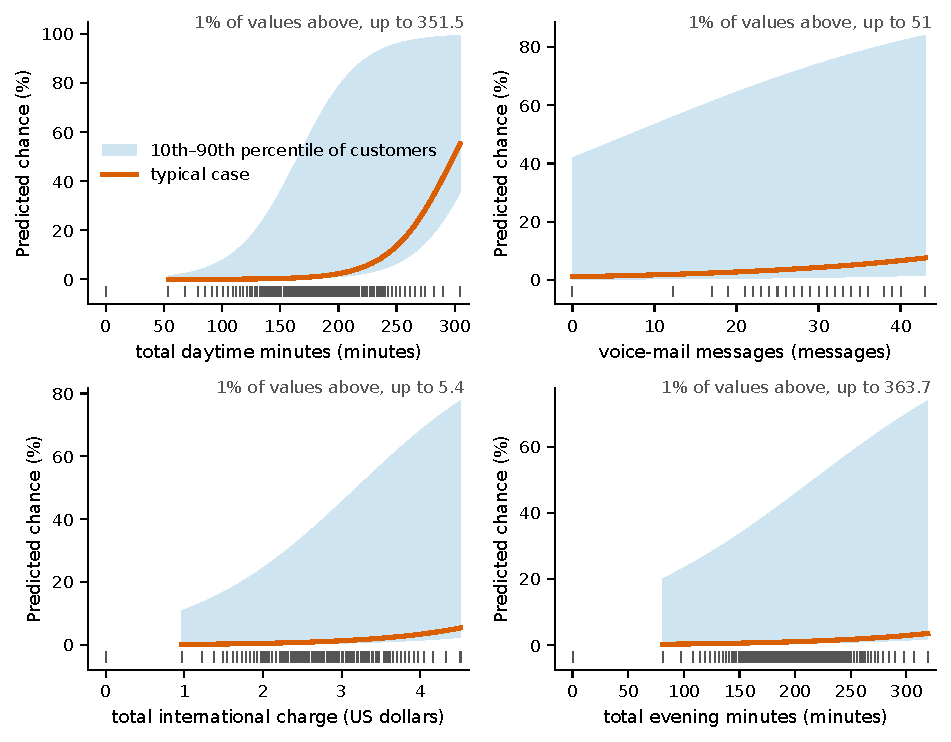
\includegraphics[width=\linewidth,height=0.88\textheight,keepaspectratio]{figures/churn100-s2-c1/ann_99-response.pdf}
\caption{Fixed-weight inputs: Response curves through this part: the typical case (bold), the 10th to 90th percentile of individual customers (band), the fold or step point (dashed) with its spread across them (grey), and the observed values (ticks).}
\label{fig:churn100s2c1:plot-ann99-0}
\end{figure}
\begin{figure}[H]\centering
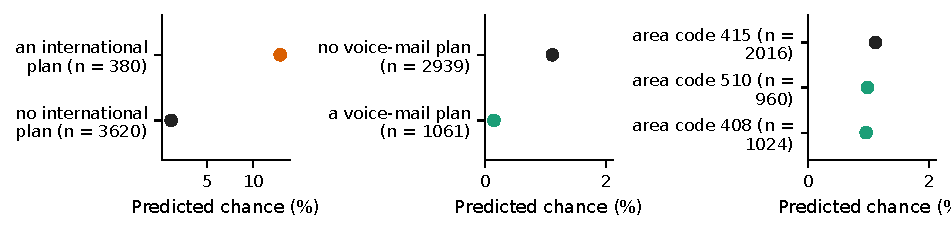
\includegraphics[width=\linewidth,height=0.88\textheight,keepaspectratio]{figures/churn100-s2-c1/ann_99-categories-small.pdf}
\caption{Fixed-weight inputs: The predicted value for the typical case at each level, through this part (n = training customers; grey: fewer than 20).}
\label{fig:churn100s2c1:plot-ann99-1}
\end{figure}
\begin{figure}[H]\centering
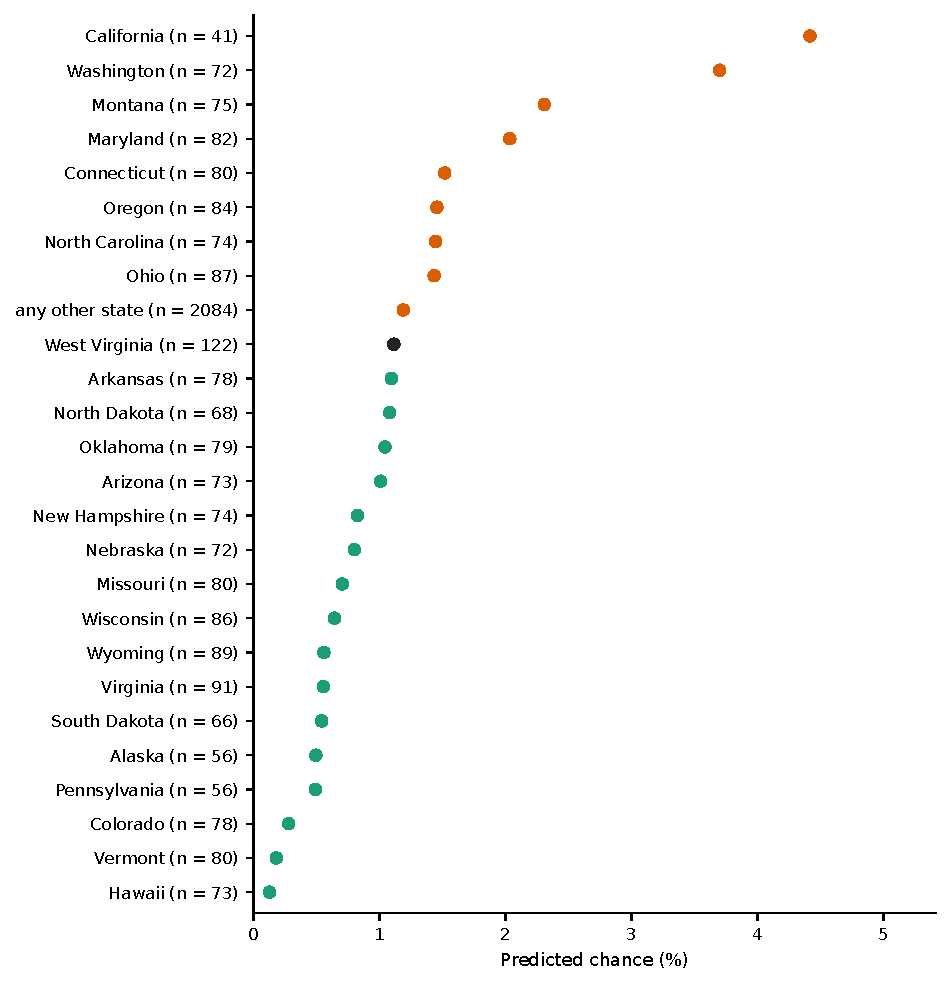
\includegraphics[width=\linewidth,height=0.88\textheight,keepaspectratio]{figures/churn100-s2-c1/ann_99-categories-C060.pdf}
\caption{Fixed-weight inputs: The predicted value for the typical case at each level, through this part (n = training customers; grey: fewer than 20).}
\label{fig:churn100s2c1:plot-ann99-2}
\end{figure}
\begin{figure}[H]\centering
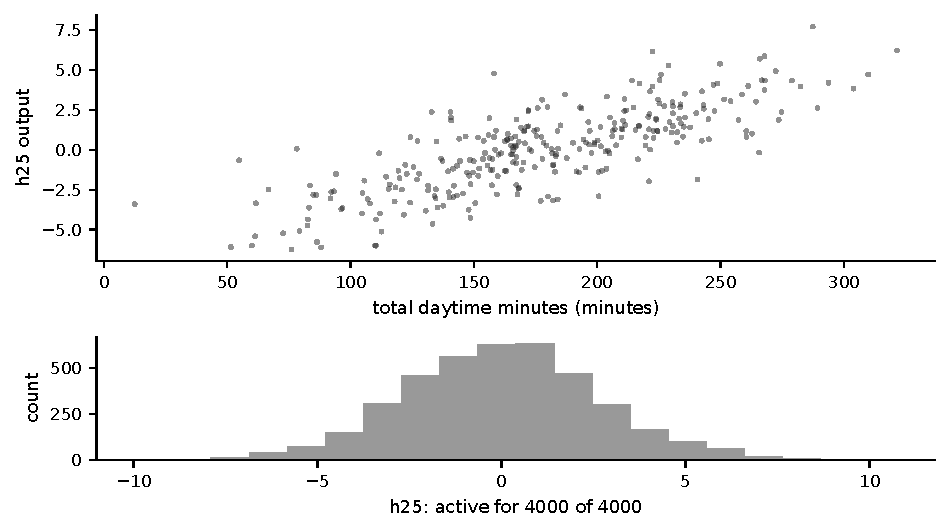
\includegraphics[width=\linewidth,height=0.88\textheight,keepaspectratio]{figures/churn100-s2-c1/ann_99-units.pdf}
\caption{Fixed-weight inputs: This part's hidden units: each unit's output against its main numeric input (top) and how often it is active (bottom).}
\label{fig:churn100s2c1:plot-ann99-3}
\end{figure}
\par\smallskip\noindent{\small Technical detail: \ref{tech:ann99}.\par}
\subsubsection{Service calls}\label{rd:ann101}
\noindent{\footnotesize Part of: The whole model (\ref{rd:ann102}).\par}
\noindent{\small Figure~\ref{fig:churn100s2c1:parts-ann101} shows what feeds this part; Figure~\ref{fig:churn100s2c1:units-ann101} its units and every connection into them (dashed boxes: connections from or to other parts, drawn in their own sections).\par}
\begin{figure}[H]\centering
\resizebox{!}{\ifdim\height>0.5\textheight 0.5\textheight\else\height\fi}{%
\resizebox{\ifdim\width>\linewidth\linewidth\else\width\fi}{!}{%
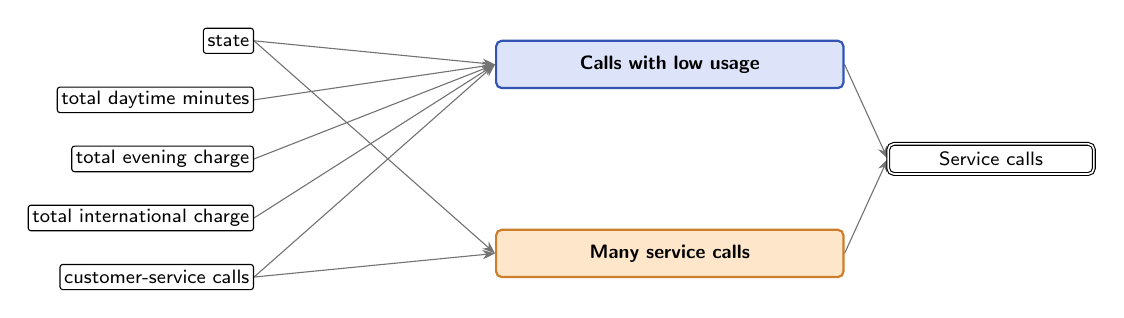
\begin{tikzpicture}[
  font=\sffamily\scriptsize, >={Stealth[length=1.6mm]},
  inp/.style={draw, rounded corners=1pt, fill=white, inner sep=1.5pt, minimum height=3.2mm, anchor=east},
  abox/.style={draw, thick, rounded corners=2pt, align=center, inner sep=3pt, minimum height=6mm, text width=42mm},
  outp/.style={draw, double, rounded corners=2pt, fill=white, align=center, inner sep=3pt, text width=24mm},
  agg/.style={draw=black!55},
]
\node[inp] (i0) at (0,1.5) {state};
\node[inp] (i1) at (0,0.75) {total daytime minutes};
\node[inp] (i2) at (0,-0.0) {total evening charge};
\node[inp] (i3) at (0,-0.75) {total international charge};
\node[inp] (i4) at (0,-1.5) {customer-service calls};
\node[abox, fill=RoyalBlue!18, draw=RoyalBlue!80!black] (b0) at (5.28,1.2) {\textbf{Calls with low usage}};
\node[abox, fill=BurntOrange!18, draw=BurntOrange!80!black] (b1) at (5.28,-1.2) {\textbf{Many service calls}};
\node[outp] (out) at (9.36,0) {Service calls};
\begin{scope}[on background layer]
\draw[->, agg, thin] (i0.east) -- (b0.west);
\draw[->, agg, thin] (i1.east) -- (b0.west);
\draw[->, agg, thin] (i2.east) -- (b0.west);
\draw[->, agg, thin] (i3.east) -- (b0.west);
\draw[->, agg, thin] (i4.east) -- (b0.west);
\draw[->, agg] (b0.east) -- (out.west);
\draw[->, agg, thin] (i0.east) -- (b1.west);
\draw[->, agg, thin] (i4.east) -- (b1.west);
\draw[->, agg] (b1.east) -- (out.west);
\end{scope}
\end{tikzpicture}}}%
\caption{Service calls: what feeds it, one level down.}
\label{fig:churn100s2c1:parts-ann101}
\end{figure}
\begin{figure}[H]\centering
\resizebox{\ifdim\width>\linewidth\linewidth\else\width\fi}{!}{%
\definecolor{netup}{HTML}{D95F02}\definecolor{netdown}{HTML}{1B9E77}\definecolor{netmixed}{HTML}{7F7F7F}%
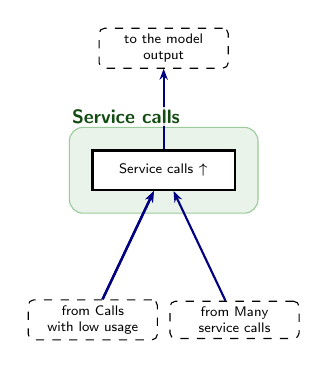
\begin{tikzpicture}[
  font=\sffamily\scriptsize, >={Stealth[length=1.4mm]},
  inp/.style={draw, circle, fill=white, minimum size=3.2mm, inner sep=0pt},
  hid/.style={draw, circle, fill=white, minimum size=5.2mm, inner sep=0.5pt, font=\sffamily\tiny},
  exitbox/.style={draw, thick, rectangle, fill=white, align=center, text width=17mm, minimum height=5mm, inner sep=1.5pt, font=\sffamily\tiny},
  sumbox/.style={draw, thick, dashed, rectangle, fill=white, align=center, text width=17mm, minimum height=5mm, inner sep=1.5pt, font=\sffamily\tiny},
  outp/.style={draw, thick, regular polygon, regular polygon sides=6, fill=white, minimum size=10mm, inner sep=0pt, font=\sffamily\tiny, align=center},
  stub/.style={draw, dashed, rounded corners=2pt, fill=white, align=center, inner sep=2pt, font=\sffamily\tiny, text width=15mm},
  inlab/.style={font=\sffamily\tiny, align=center, text width=15mm, inner sep=1pt, fill=white, fill opacity=0.8, text opacity=1},
  wpos/.style={draw=NavyBlue}, wneg/.style={draw=BrickRed}, wagg/.style={draw=black!45, line width=1.2pt},
  wmix/.style={draw=Plum},
]
\node[exitbox] (nidentityxsvc) at (1.8,1.9) {Service calls $\uparrow$};
\node[stub] (nfromxxCallsxwithxlowxusage) at (0.9,0.0) {from Calls with low usage};
\node[stub] (nfromxxManyxservicexcalls) at (2.7,0.0) {from Many service calls};
\node[stub] (ntoxxthexmodelxoutput) at (1.8,3.45) {to the model output};
\begin{scope}[on background layer]
\node[fit=(nidentityxsvc) , inner sep=8pt, rounded corners=5pt, fill=ForestGreen!10, draw=ForestGreen!45] (clu0) {};
\draw[->, wpos, line width=0.81pt] (nfromxxCallsxwithxlowxusage) -- (nidentityxsvc);
\draw[->, wpos, line width=0.88pt] (nfromxxCallsxwithxlowxusage) -- (nidentityxsvc);
\draw[->, wpos, line width=0.77pt] (nfromxxManyxservicexcalls) -- (nidentityxsvc);
\draw[->, wpos, line width=0.60pt] (nidentityxsvc) -- (ntoxxthexmodelxoutput);
\end{scope}
\node[font=\sffamily\scriptsize\bfseries, text=ForestGreen!55!black, anchor=south west, inner sep=1pt, fill=white, fill opacity=0.85, text opacity=1] at (clu0.north west) {Service calls};
\end{tikzpicture}}%
\caption{Service calls: its units and every connection into them. Blue: positive weight (raises the score); red: negative weight (lowers it); thicker: larger weight. Orange outline and up arrow: raises the final prediction; teal and down arrow: lowers it; grey and double arrow: depends.}
\label{fig:churn100s2c1:units-ann101}
\end{figure}
\paragraph{Hypothesis.} This part raises the chance of leaving with calls to customer service, from 4 calls upwards and in an uneven way, and more so for customers with low daytime use; it adds up two parts.\,{\scriptsize\textcolor{NavyBlue}{[C111, C108, C107]}}
\paragraph{Evidence.} It is made of two parts that are added: calls with low usage, and many service calls.\,{\scriptsize\textcolor{NavyBlue}{[C111]}} Through it, daytime minutes lower a typical customer's chance only while they stay below about 170 minutes (between 147 and 216 minutes for different customers), in an uneven way, from about 38\% at 91 minutes to about 1\% at 352 minutes.\,{\scriptsize\textcolor{NavyBlue}{[C107]}} Customer-service calls add to it from 4 calls upwards, in an uneven way: for a typical such customer, from about 3\% at 0 calls to about 11\% at 4 calls.\,{\scriptsize\textcolor{NavyBlue}{[C108]}} With an evening charge above 17.12 US dollars, the chance is lowest at about 154 minutes of daytime use and higher either side: from about 1\% at 112 minutes to about 17\% at 249 minutes, against about 2\% to about 10\% at or below that charge.\,{\scriptsize\textcolor{NavyBlue}{[C103]}}
\par\noindent{\small Evidence plots: Figure~\ref{fig:churn100s2c1:plot-ann101-0}, Figure~\ref{fig:churn100s2c1:plot-ann101-1}, Figure~\ref{fig:churn100s2c1:plot-ann101-2}, Figure~\ref{fig:churn100s2c1:plot-ann101-3}, Figure~\ref{fig:churn100s2c1:plot-ann101-4}, Figure~\ref{fig:churn100s2c1:plot-ann101-5}, Figure~\ref{fig:churn100s2c1:plot-ann101-6}, Figure~\ref{fig:churn100s2c1:plot-ann101-7}.\par}
\par\noindent{\small Figure~\ref{fig:churn100s2c1:plot-ann101-6} shows this part's own output, unit h26: over its two main inputs, with the line where it switches on.\par}
\begin{figure}[H]\centering
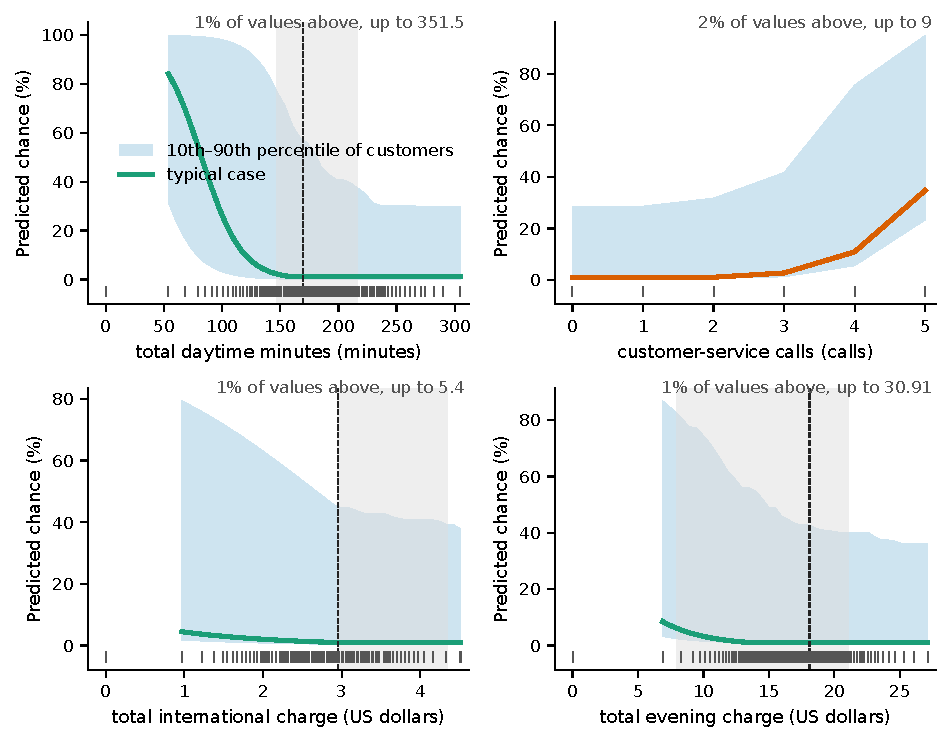
\includegraphics[width=\linewidth,height=0.88\textheight,keepaspectratio]{figures/churn100-s2-c1/ann_101-response.pdf}
\caption{Service calls: Response curves through this part: the typical case (bold), the 10th to 90th percentile of individual customers (band), the fold or step point (dashed) with its spread across them (grey), and the observed values (ticks).}
\label{fig:churn100s2c1:plot-ann101-0}
\end{figure}
\begin{figure}[H]\centering
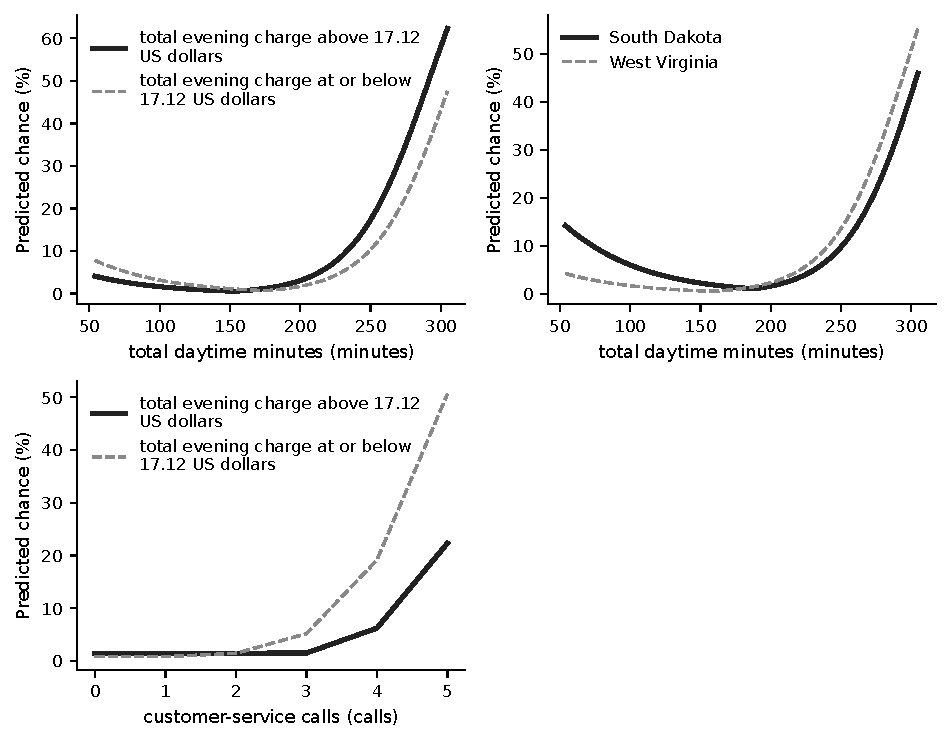
\includegraphics[width=\linewidth,height=0.88\textheight,keepaspectratio]{figures/churn100-s2-c1/ann_101-interaction.pdf}
\caption{Service calls: How the effect differs between groups: one curve per group, for the typical case of each group.}
\label{fig:churn100s2c1:plot-ann101-1}
\end{figure}
\begin{figure}[H]\centering
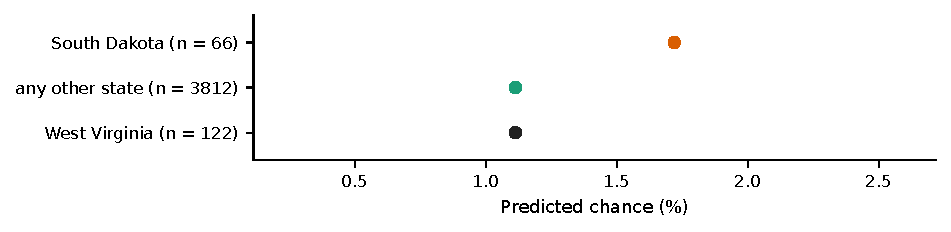
\includegraphics[width=\linewidth,height=0.88\textheight,keepaspectratio]{figures/churn100-s2-c1/ann_101-categories-small.pdf}
\caption{Service calls: The predicted value for the typical case at each level, through this part (n = training customers; grey: fewer than 20).}
\label{fig:churn100s2c1:plot-ann101-2}
\end{figure}
\begin{figure}[H]\centering
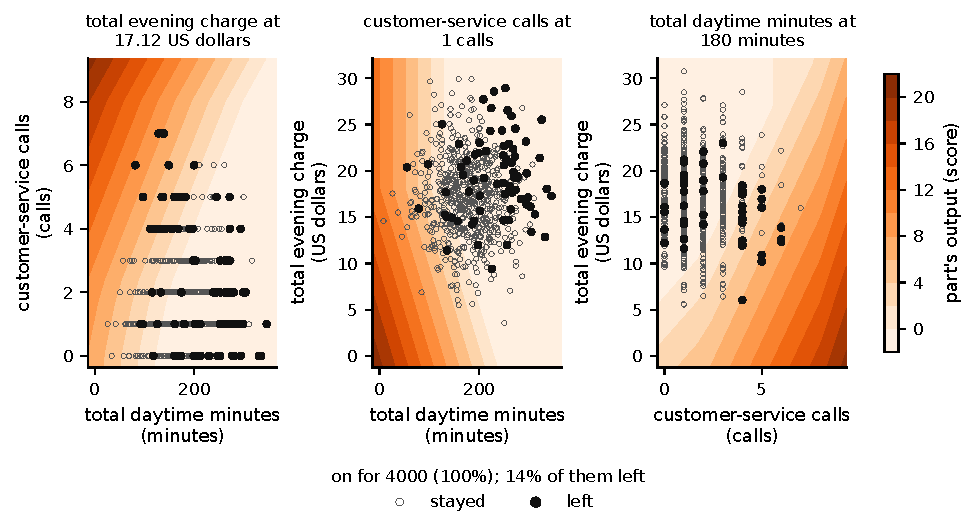
\includegraphics[width=\linewidth,height=0.88\textheight,keepaspectratio]{figures/churn100-s2-c1/ann_101-deep-map.pdf}
\caption{Service calls: The part's own output over each pair of its three main inputs (the third held at its median, named above each panel; the points are the training rows whose third input is between its 40th and 60th percentile), other inputs at the typical case: colour where it is on, flat grey where it is switched off, the black line where it switches on; training customers as hollow (no event) and filled (event) points, so the part can be seen catching the events (the predicted-chance overlay was harder to read). The switch-on line is traced on this map only; the boundary claim (C162) did not pass its check on the data, so no rule is stated.}
\label{fig:churn100s2c1:plot-ann101-3}
\end{figure}
\begin{figure}[H]\centering
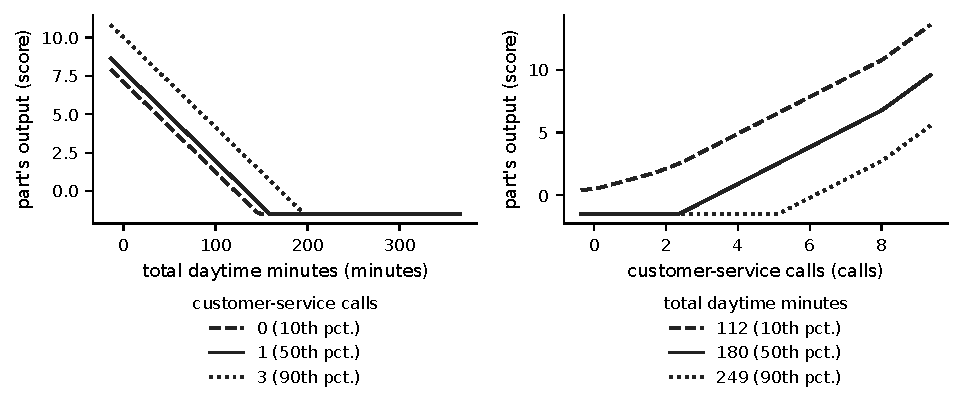
\includegraphics[width=\linewidth,height=0.88\textheight,keepaspectratio]{figures/churn100-s2-c1/ann_101-deep-slices.pdf}
\caption{Service calls: Slices of the same map: the part's own output against each input at three values of the other, so the tilted boundary shows as a shifting hinge. The switch-on line is traced on this map only; the boundary claim (C162) did not pass its check on the data, so no rule is stated.}
\label{fig:churn100s2c1:plot-ann101-4}
\end{figure}
\begin{figure}[H]\centering
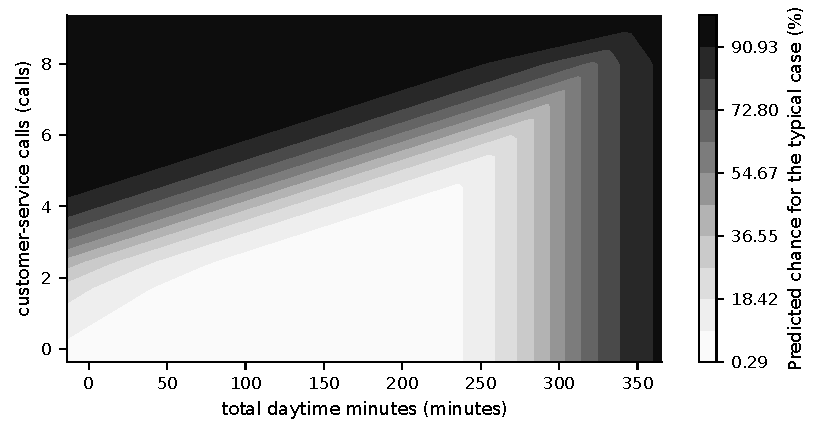
\includegraphics[width=\linewidth,height=0.88\textheight,keepaspectratio]{figures/churn100-s2-c1/ann_101-deep-risk.pdf}
\caption{Service calls: The same map on the final scale: the predicted value for the typical case, with the switch-on line (orange). The switch-on line is traced on this map only; the boundary claim (C162) did not pass its check on the data, so no rule is stated.}
\label{fig:churn100s2c1:plot-ann101-5}
\end{figure}
\begin{figure}[H]\centering
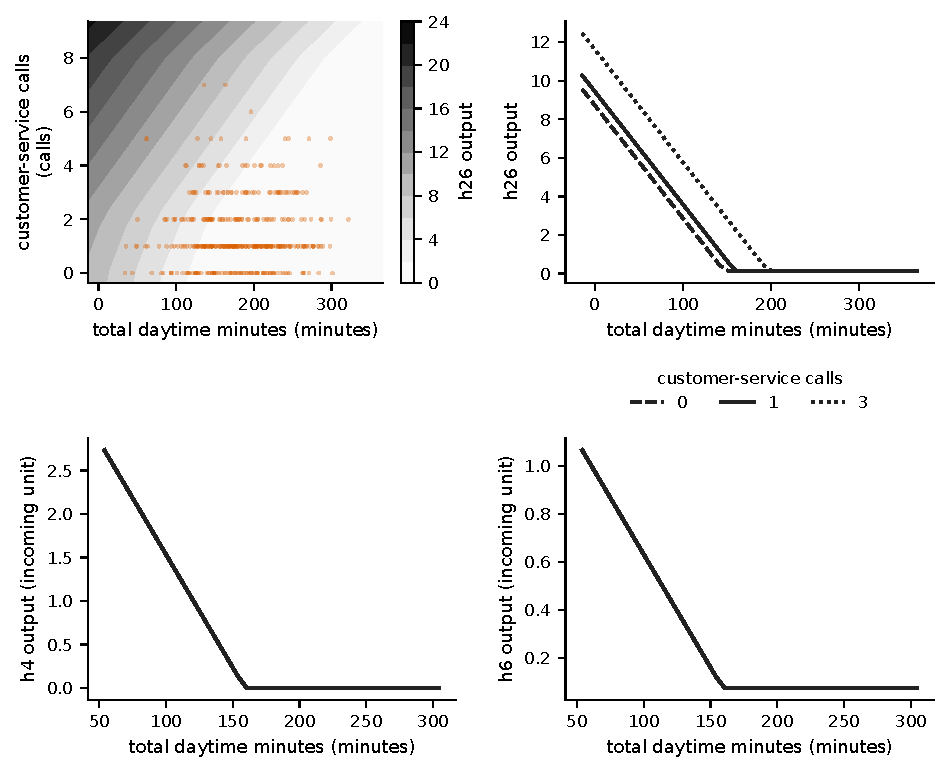
\includegraphics[width=\linewidth,height=0.88\textheight,keepaspectratio]{figures/churn100-s2-c1/ann_101-partial-identity_svc.pdf}
\caption{Service calls: This part's own output, unit h26 (combines 3 non-linear units), on its own scale (its activation), with every other input at the typical case; it is active for 3145 of 4000. Left: its output over its two main inputs (orange line: where it switches on; dots: the data); right: slices at three values of the second input; then each incoming non-linear unit against its own main input.}
\label{fig:churn100s2c1:plot-ann101-6}
\end{figure}
\begin{figure}[H]\centering
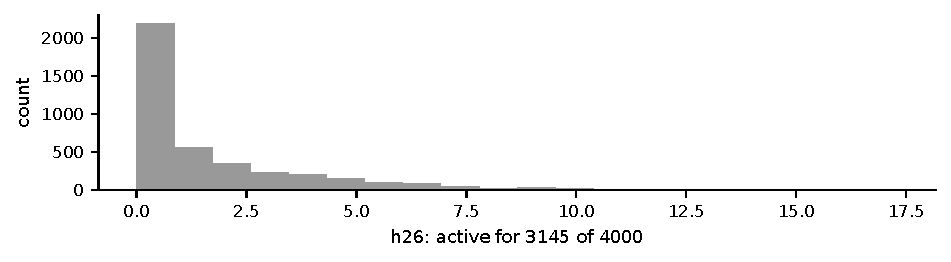
\includegraphics[width=\linewidth,height=0.88\textheight,keepaspectratio]{figures/churn100-s2-c1/ann_101-units.pdf}
\caption{Service calls: This part's hidden units: each unit's output against its main numeric input (top) and how often it is active (bottom).}
\label{fig:churn100s2c1:plot-ann101-7}
\end{figure}
\par\smallskip\noindent{\small \textbf{Dive deeper:} Calls with low usage (\ref{rd:ann91}); Many service calls (\ref{rd:ann93}). Technical detail: \ref{tech:ann101}.\par}
\subsubsection{Calls with low usage}\label{rd:ann91}
\noindent{\footnotesize Part of: Service calls (\ref{rd:ann101}).\par}
\noindent{\small Figure~\ref{fig:churn100s2c1:parts-ann91} shows what feeds this part; Figure~\ref{fig:churn100s2c1:units-ann91} its units and every connection into them (dashed boxes: connections from or to other parts, drawn in their own sections).\par}
\begin{figure}[H]\centering
\resizebox{!}{\ifdim\height>0.5\textheight 0.5\textheight\else\height\fi}{%
\resizebox{\ifdim\width>\linewidth\linewidth\else\width\fi}{!}{%
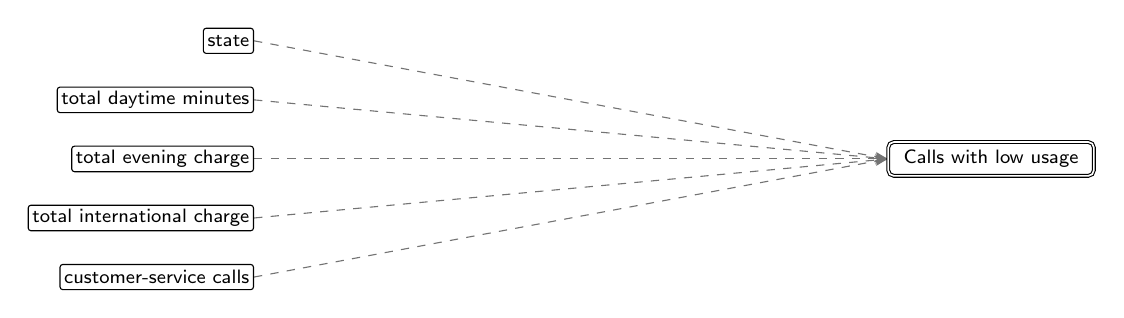
\begin{tikzpicture}[
  font=\sffamily\scriptsize, >={Stealth[length=1.6mm]},
  inp/.style={draw, rounded corners=1pt, fill=white, inner sep=1.5pt, minimum height=3.2mm, anchor=east},
  abox/.style={draw, thick, rounded corners=2pt, align=center, inner sep=3pt, minimum height=6mm, text width=42mm},
  outp/.style={draw, double, rounded corners=2pt, fill=white, align=center, inner sep=3pt, text width=24mm},
  agg/.style={draw=black!55},
]
\node[inp] (i0) at (0,1.5) {state};
\node[inp] (i1) at (0,0.75) {total daytime minutes};
\node[inp] (i2) at (0,-0.0) {total evening charge};
\node[inp] (i3) at (0,-0.75) {total international charge};
\node[inp] (i4) at (0,-1.5) {customer-service calls};
\node[outp] (out) at (9.36,0) {Calls with low usage};
\begin{scope}[on background layer]
\draw[->, agg, thin, dashed] (i0.east) -- (out.west);
\draw[->, agg, thin, dashed] (i1.east) -- (out.west);
\draw[->, agg, thin, dashed] (i2.east) -- (out.west);
\draw[->, agg, thin, dashed] (i3.east) -- (out.west);
\draw[->, agg, thin, dashed] (i4.east) -- (out.west);
\end{scope}
\end{tikzpicture}}}%
\caption{Calls with low usage: what feeds it, one level down.}
\label{fig:churn100s2c1:parts-ann91}
\end{figure}
\begin{figure}[H]\centering
\resizebox{\ifdim\width>\linewidth\linewidth\else\width\fi}{!}{%
\definecolor{netup}{HTML}{D95F02}\definecolor{netdown}{HTML}{1B9E77}\definecolor{netmixed}{HTML}{7F7F7F}%
\begin{tikzpicture}[
  font=\sffamily\scriptsize, >={Stealth[length=1.4mm]},
  inp/.style={draw, circle, fill=white, minimum size=3.2mm, inner sep=0pt},
  hid/.style={draw, circle, fill=white, minimum size=5.2mm, inner sep=0.5pt, font=\sffamily\tiny},
  exitbox/.style={draw, thick, rectangle, fill=white, align=center, text width=17mm, minimum height=5mm, inner sep=1.5pt, font=\sffamily\tiny},
  sumbox/.style={draw, thick, dashed, rectangle, fill=white, align=center, text width=17mm, minimum height=5mm, inner sep=1.5pt, font=\sffamily\tiny},
  outp/.style={draw, thick, regular polygon, regular polygon sides=6, fill=white, minimum size=10mm, inner sep=0pt, font=\sffamily\tiny, align=center},
  stub/.style={draw, dashed, rounded corners=2pt, fill=white, align=center, inner sep=2pt, font=\sffamily\tiny, text width=15mm},
  inlab/.style={font=\sffamily\tiny, align=center, text width=15mm, inner sep=1pt, fill=white, fill opacity=0.8, text opacity=1},
  wpos/.style={draw=NavyBlue}, wneg/.style={draw=BrickRed}, wagg/.style={draw=black!45, line width=1.2pt},
  wmix/.style={draw=Plum},
]
\node[hid] (n12926) at (3.75,1.9) {h17};
\node[hid] (n2796) at (5.25,3.25) {h7};
\node[hid] (n807) at (4.5,4.6) {h4};
\node[hid] (n2627xb) at (3.75,3.25) {h22};
\node[hid] (n1264) at (4.5,5.95) {h6};
\node[hid] (n9555xb) at (5.25,1.9) {h24};
\node[inp, draw=netdown, very thick] (ninxxtotalxintlxcharge) at (4.5,0.0) {};
\path (ninxxtotalxintlxcharge.south) node[inlab, anchor=north] (labninxxtotalxintlxcharge) {total international charge $\downarrow$};
\node[inp, draw=netdown, very thick] (ninxxtotalxevexcharge) at (8.1,0.0) {};
\path (ninxxtotalxevexcharge.south) node[inlab, anchor=north] (labninxxtotalxevexcharge) {total evening charge $\downarrow$};
\node[inp, draw=netdown, very thick] (ninxxtotalxdayxminutes) at (2.7,0.0) {};
\path (ninxxtotalxdayxminutes.south) node[inlab, anchor=north] (labninxxtotalxdayxminutes) {total daytime minutes $\downarrow$};
\node[inp, draw=netmixed, very thick] (ngrpxxstate) at (6.3,0.0) {};
\path (ngrpxxstate.south) node[inlab, anchor=north] (labngrpxxstate) {state (31 of 51 used) $\updownarrow$};
\node[inp, draw=netup, very thick] (ninxxnumberxcustomerxservicexcalls) at (0.9,0.0) {};
\path (ninxxnumberxcustomerxservicexcalls.south) node[inlab, anchor=north] (labninxxnumberxcustomerxservicexcalls) {customer-service calls $\uparrow$};
\node[stub] (ntoxxServicexcalls) at (4.5,7.5) {to Service calls};
\begin{scope}[on background layer]
\node[fit=(n12926) (n2796) (n807) (n2627xb) (n1264) (n9555xb) , inner sep=8pt, rounded corners=5pt, fill=ForestGreen!10, draw=ForestGreen!45] (clu0) {};
\draw[->, wpos, line width=0.47pt] (n2796) -- (n807);
\draw[->, wpos, line width=0.38pt] (n807) -- (n1264);
\draw[->, wpos, line width=0.37pt] (n12926) -- (n2796);
\draw[->, wpos, line width=0.49pt] (n2627xb) -- (n807);
\draw[->, wpos, line width=0.36pt] (n9555xb) -- (n2627xb);
\draw[->, wneg, line width=0.36pt] (ninxxtotalxintlxcharge) -- (n1264);
\draw[->, wneg, line width=0.60pt] (ninxxtotalxevexcharge) -- (n2796);
\draw[->, wneg, line width=0.74pt] (ninxxtotalxdayxminutes) -- (n807);
\draw[->, wpos, line width=0.26pt] (ninxxnumberxcustomerxservicexcalls) -- (n807);
\draw[->, wpos, line width=0.38pt] (ninxxnumberxcustomerxservicexcalls) -- (n2796);
\draw[->, wpos, line width=0.60pt] (ninxxnumberxcustomerxservicexcalls) -- (n12926);
\draw[->, wpos, line width=0.35pt] (ninxxnumberxcustomerxservicexcalls) -- (n2627xb);
\draw[->, wpos, line width=0.55pt] (ninxxnumberxcustomerxservicexcalls) -- (n9555xb);
\draw[->, wpos, line width=0.81pt] (n807) -- (ntoxxServicexcalls);
\draw[->, wpos, line width=0.88pt] (n1264) -- (ntoxxServicexcalls);
\draw[->, wpos, line width=0.30pt] (ngrpxxstate) -- node[pos=0.8, sloped, above, font=\sffamily\tiny, inner sep=1pt, fill=white, fill opacity=0.8, text opacity=1] {+0.15} (n2796);
\end{scope}
\node[font=\sffamily\scriptsize\bfseries, text=ForestGreen!55!black, anchor=south west, inner sep=1pt, fill=white, fill opacity=0.85, text opacity=1] at (clu0.north west) {Calls with low usage};
\end{tikzpicture}}%
\caption{Calls with low usage: its units and every connection into them. Blue: positive weight (raises the score); red: negative weight (lowers it); thicker: larger weight. Orange outline and up arrow: raises the final prediction; teal and down arrow: lowers it; grey and double arrow: depends.}
\label{fig:churn100s2c1:units-ann91}
\end{figure}
\paragraph{Hypothesis.} This part raises the chance of leaving for customers with low usage, more so when they call customer service: daytime minutes lower it only while they stay below about 170 minutes (between 147 and 216 minutes for different customers), and calls raise it, both in an uneven way.\,{\scriptsize\textcolor{NavyBlue}{[C119, C113]}}
\paragraph{Evidence.} It acts on 3121 of 4000 training customers, 402 of whom left; for the typical customer it acts on, it changes the chance by less than a point.\,{\scriptsize\textcolor{NavyBlue}{[C123]}} Through it, a typical customer's chance falls in an uneven way from about 38\% at 91 minutes of daytime use to about 1\% at 352 minutes, with no further fall past about 170 minutes (between 147 and 216 minutes for different customers).\,{\scriptsize\textcolor{NavyBlue}{[C119]}} A higher international charge lowers it only while it stays below about 2.95 US dollars (between 2.95 and 4.34 US dollars for different customers), in an uneven way, from about 3\% to about 1\%.\,{\scriptsize\textcolor{NavyBlue}{[C121]}} Customer-service calls raise it in an uneven way, from about 1\% at 0 calls to about 3\% at 3 calls.\,{\scriptsize\textcolor{NavyBlue}{[C113]}} Its formula reproduces the part exactly on all 4000 training customers.\,{\scriptsize\textcolor{NavyBlue}{[C124]}}
\par\noindent{\small Evidence plots: Figure~\ref{fig:churn100s2c1:plot-ann91-0}, Figure~\ref{fig:churn100s2c1:plot-ann91-1}, Figure~\ref{fig:churn100s2c1:plot-ann91-2}, Figure~\ref{fig:churn100s2c1:plot-ann91-3}, Figure~\ref{fig:churn100s2c1:plot-ann91-4}, Figure~\ref{fig:churn100s2c1:plot-ann91-5}, Figure~\ref{fig:churn100s2c1:plot-ann91-6}, Figure~\ref{fig:churn100s2c1:plot-ann91-7}, Figure~\ref{fig:churn100s2c1:plot-ann91-8}.\par}
\par\noindent{\small Figure~\ref{fig:churn100s2c1:plot-ann91-6} shows this part's own output, unit h4: over its two main inputs, with the line where it switches on.\par}
\par\noindent{\small Figure~\ref{fig:churn100s2c1:plot-ann91-7} shows this part's own output, unit h6: over its two main inputs, with the line where it switches on.\par}
\begin{figure}[H]\centering
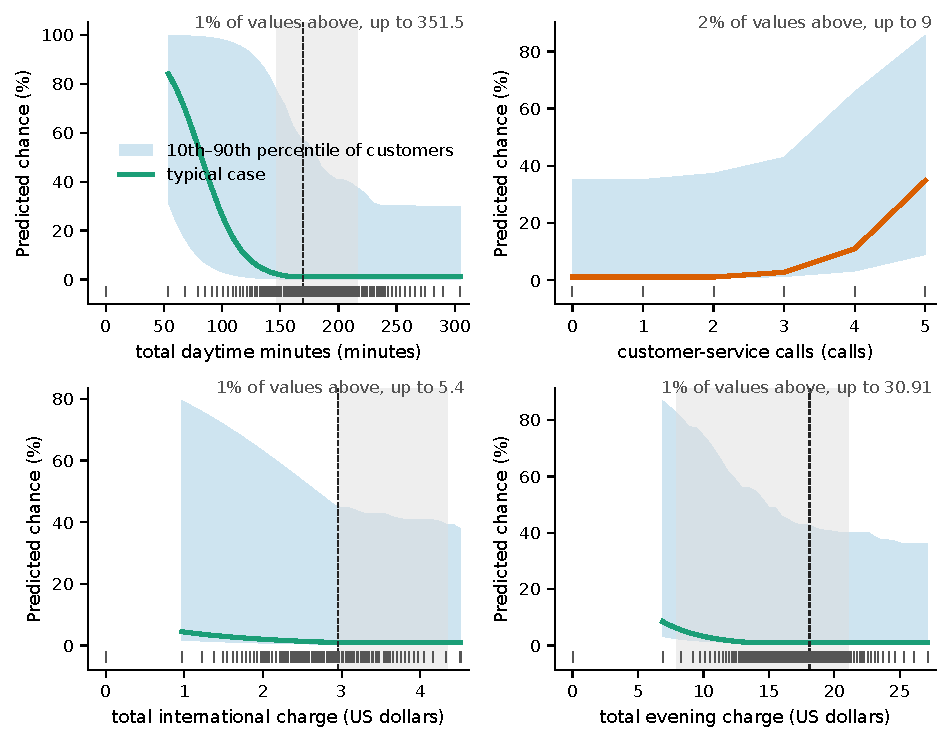
\includegraphics[width=\linewidth,height=0.88\textheight,keepaspectratio]{figures/churn100-s2-c1/ann_91-response.pdf}
\caption{Calls with low usage: Response curves through this part: the typical case (bold), the 10th to 90th percentile of individual customers (band), the fold or step point (dashed) with its spread across them (grey), and the observed values (ticks).}
\label{fig:churn100s2c1:plot-ann91-0}
\end{figure}
\begin{figure}[H]\centering
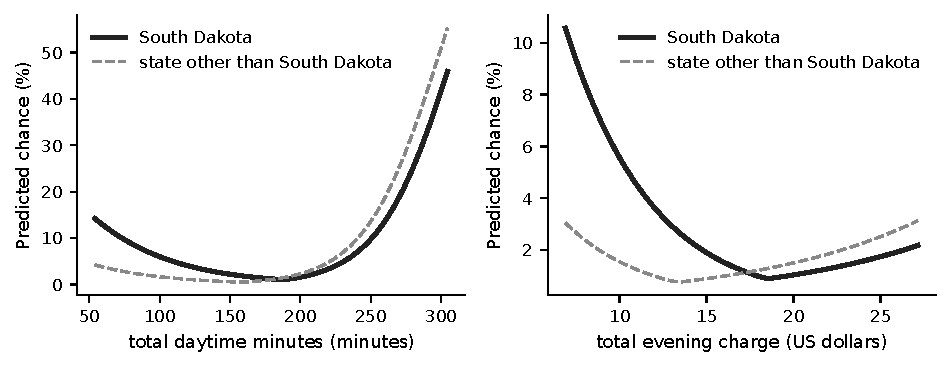
\includegraphics[width=\linewidth,height=0.88\textheight,keepaspectratio]{figures/churn100-s2-c1/ann_91-interaction.pdf}
\caption{Calls with low usage: How the effect differs between groups: one curve per group, for the typical case of each group.}
\label{fig:churn100s2c1:plot-ann91-1}
\end{figure}
\begin{figure}[H]\centering
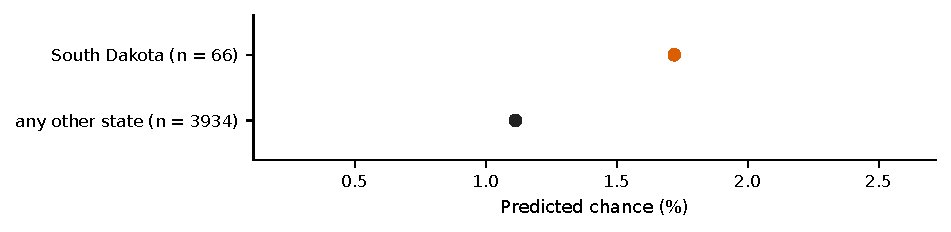
\includegraphics[width=\linewidth,height=0.88\textheight,keepaspectratio]{figures/churn100-s2-c1/ann_91-categories-small.pdf}
\caption{Calls with low usage: The predicted value for the typical case at each level, through this part (n = training customers; grey: fewer than 20).}
\label{fig:churn100s2c1:plot-ann91-2}
\end{figure}
\begin{figure}[H]\centering
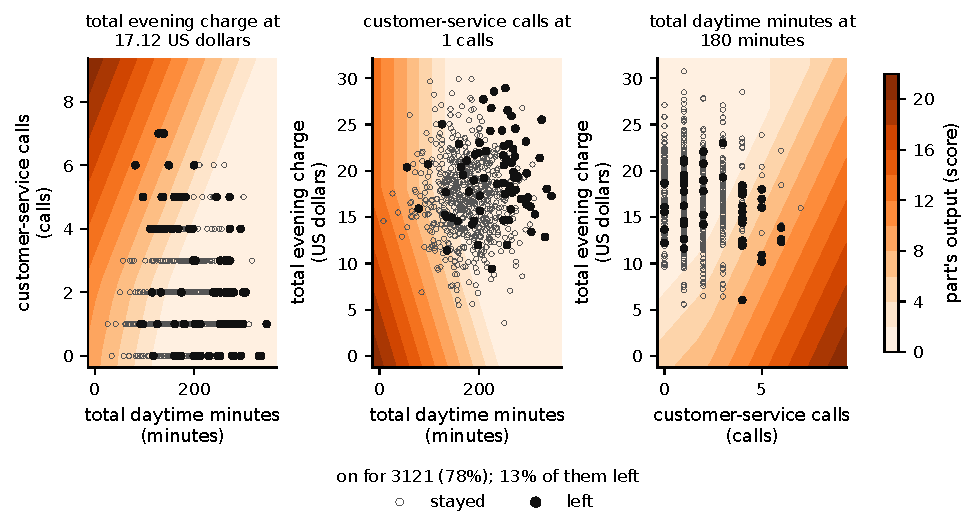
\includegraphics[width=\linewidth,height=0.88\textheight,keepaspectratio]{figures/churn100-s2-c1/ann_91-deep-map.pdf}
\caption{Calls with low usage: The part's own output over each pair of its three main inputs (the third held at its median, named above each panel; the points are the training rows whose third input is between its 40th and 60th percentile), other inputs at the typical case: colour where it is on, flat grey where it is switched off, the black line where it switches on; training customers as hollow (no event) and filled (event) points, so the part can be seen catching the events (the predicted-chance overlay was harder to read). The switch-on line is traced on this map only; the boundary claim (C163) did not pass its check on the data, so no rule is stated.}
\label{fig:churn100s2c1:plot-ann91-3}
\end{figure}
\begin{figure}[H]\centering
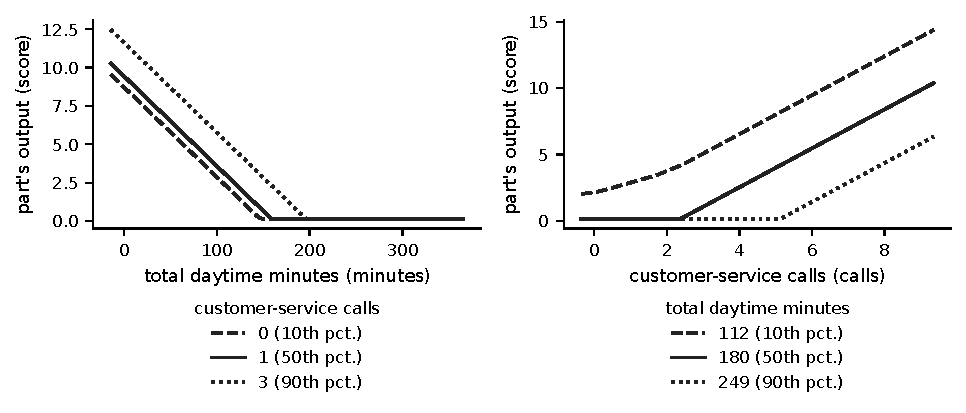
\includegraphics[width=\linewidth,height=0.88\textheight,keepaspectratio]{figures/churn100-s2-c1/ann_91-deep-slices.pdf}
\caption{Calls with low usage: Slices of the same map: the part's own output against each input at three values of the other, so the tilted boundary shows as a shifting hinge. The switch-on line is traced on this map only; the boundary claim (C163) did not pass its check on the data, so no rule is stated.}
\label{fig:churn100s2c1:plot-ann91-4}
\end{figure}
\begin{figure}[H]\centering
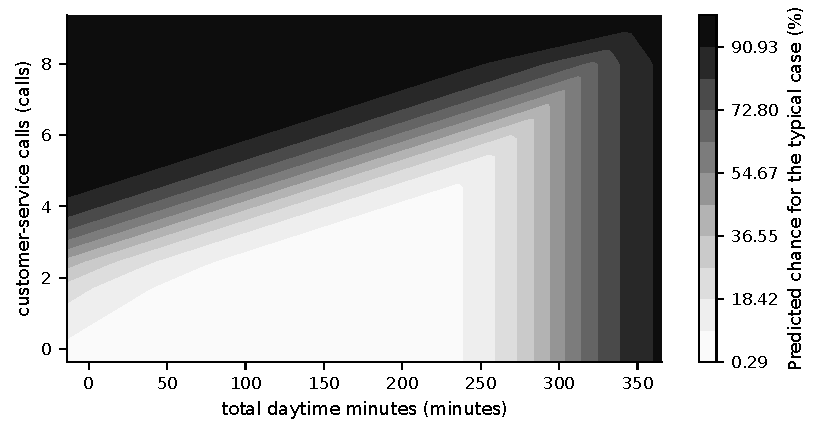
\includegraphics[width=\linewidth,height=0.88\textheight,keepaspectratio]{figures/churn100-s2-c1/ann_91-deep-risk.pdf}
\caption{Calls with low usage: The same map on the final scale: the predicted value for the typical case, with the switch-on line (orange). The switch-on line is traced on this map only; the boundary claim (C163) did not pass its check on the data, so no rule is stated.}
\label{fig:churn100s2c1:plot-ann91-5}
\end{figure}
\begin{figure}[H]\centering
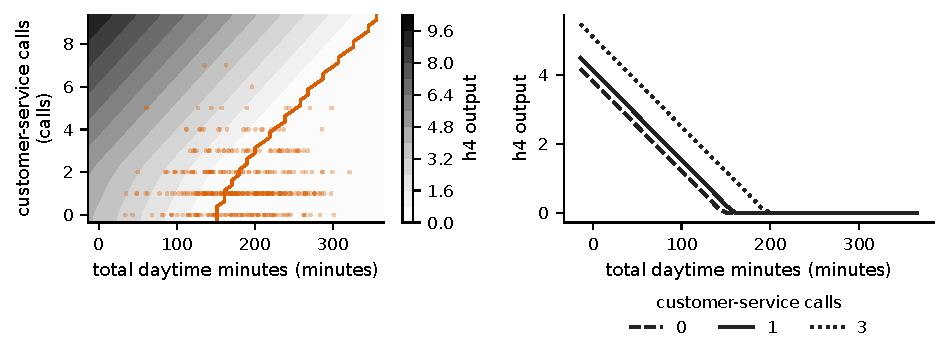
\includegraphics[width=\linewidth,height=0.88\textheight,keepaspectratio]{figures/churn100-s2-c1/ann_91-partial-807.pdf}
\caption{Calls with low usage: This part's own output, unit h4 (the output of 'Calls with low usage'), on its own scale (its activation), with every other input at the typical case; it is active for 1840 of 4000. Left: its output over its two main inputs (orange line: where it switches on; dots: the data); right: slices at three values of the second input.}
\label{fig:churn100s2c1:plot-ann91-6}
\end{figure}
\begin{figure}[H]\centering
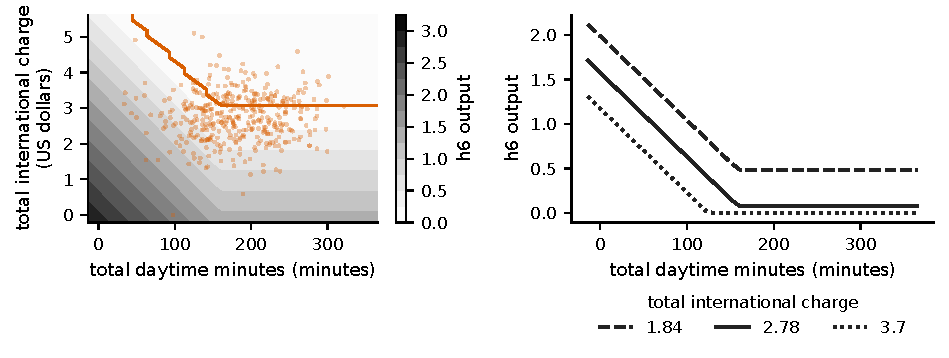
\includegraphics[width=\linewidth,height=0.88\textheight,keepaspectratio]{figures/churn100-s2-c1/ann_91-partial-1264.pdf}
\caption{Calls with low usage: This part's own output, unit h6 (the output of 'Calls with low usage'), on its own scale (its activation), with every other input at the typical case; it is active for 2901 of 4000. Left: its output over its two main inputs (orange line: where it switches on; dots: the data); right: slices at three values of the second input.}
\label{fig:churn100s2c1:plot-ann91-7}
\end{figure}
\begin{figure}[H]\centering
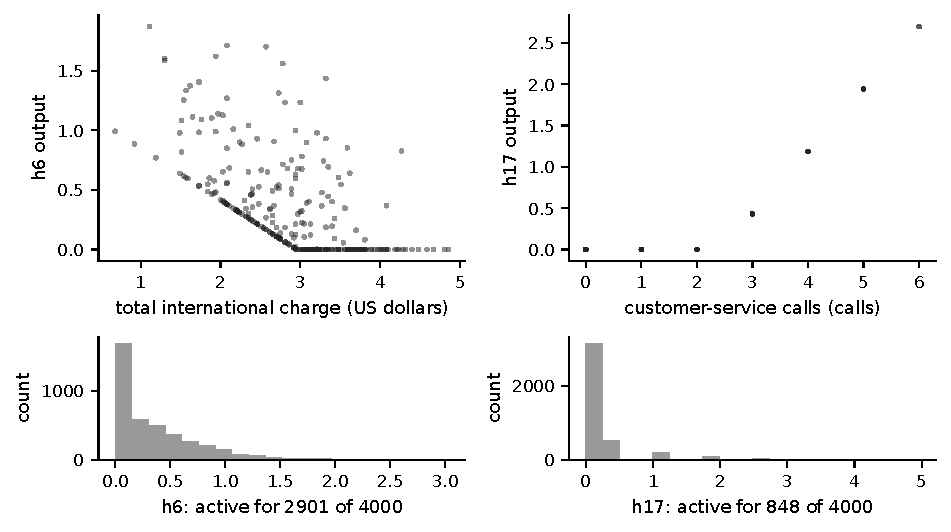
\includegraphics[width=\linewidth,height=0.88\textheight,keepaspectratio]{figures/churn100-s2-c1/ann_91-units.pdf}
\caption{Calls with low usage: This part's hidden units: each unit's output against its main numeric input (top) and how often it is active (bottom).}
\label{fig:churn100s2c1:plot-ann91-8}
\end{figure}
\par\smallskip\noindent{\small Technical detail: \ref{tech:ann91}.\par}
\subsubsection{Many service calls}\label{rd:ann93}
\noindent{\footnotesize Part of: Service calls (\ref{rd:ann101}).\par}
\noindent{\small Figure~\ref{fig:churn100s2c1:parts-ann93} shows what feeds this part; Figure~\ref{fig:churn100s2c1:units-ann93} its units and every connection into them (dashed boxes: connections from or to other parts, drawn in their own sections).\par}
\begin{figure}[H]\centering
\resizebox{!}{\ifdim\height>0.5\textheight 0.5\textheight\else\height\fi}{%
\resizebox{\ifdim\width>\linewidth\linewidth\else\width\fi}{!}{%
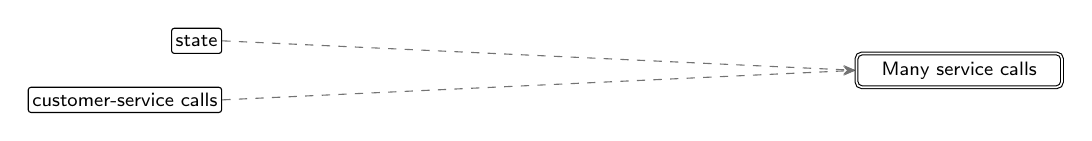
\begin{tikzpicture}[
  font=\sffamily\scriptsize, >={Stealth[length=1.6mm]},
  inp/.style={draw, rounded corners=1pt, fill=white, inner sep=1.5pt, minimum height=3.2mm, anchor=east},
  abox/.style={draw, thick, rounded corners=2pt, align=center, inner sep=3pt, minimum height=6mm, text width=42mm},
  outp/.style={draw, double, rounded corners=2pt, fill=white, align=center, inner sep=3pt, text width=24mm},
  agg/.style={draw=black!55},
]
\node[inp] (i0) at (0,0.375) {state};
\node[inp] (i1) at (0,-0.375) {customer-service calls};
\node[outp] (out) at (9.36,0) {Many service calls};
\begin{scope}[on background layer]
\draw[->, agg, thin, dashed] (i0.east) -- (out.west);
\draw[->, agg, thin, dashed] (i1.east) -- (out.west);
\end{scope}
\end{tikzpicture}}}%
\caption{Many service calls: what feeds it, one level down.}
\label{fig:churn100s2c1:parts-ann93}
\end{figure}
\begin{figure}[H]\centering
\resizebox{\ifdim\width>\linewidth\linewidth\else\width\fi}{!}{%
\definecolor{netup}{HTML}{D95F02}\definecolor{netdown}{HTML}{1B9E77}\definecolor{netmixed}{HTML}{7F7F7F}%
\begin{tikzpicture}[
  font=\sffamily\scriptsize, >={Stealth[length=1.4mm]},
  inp/.style={draw, circle, fill=white, minimum size=3.2mm, inner sep=0pt},
  hid/.style={draw, circle, fill=white, minimum size=5.2mm, inner sep=0.5pt, font=\sffamily\tiny},
  exitbox/.style={draw, thick, rectangle, fill=white, align=center, text width=17mm, minimum height=5mm, inner sep=1.5pt, font=\sffamily\tiny},
  sumbox/.style={draw, thick, dashed, rectangle, fill=white, align=center, text width=17mm, minimum height=5mm, inner sep=1.5pt, font=\sffamily\tiny},
  outp/.style={draw, thick, regular polygon, regular polygon sides=6, fill=white, minimum size=10mm, inner sep=0pt, font=\sffamily\tiny, align=center},
  stub/.style={draw, dashed, rounded corners=2pt, fill=white, align=center, inner sep=2pt, font=\sffamily\tiny, text width=15mm},
  inlab/.style={font=\sffamily\tiny, align=center, text width=15mm, inner sep=1pt, fill=white, fill opacity=0.8, text opacity=1},
  wpos/.style={draw=NavyBlue}, wneg/.style={draw=BrickRed}, wagg/.style={draw=black!45, line width=1.2pt},
  wmix/.style={draw=Plum},
]
\node[exitbox] (n7208) at (1.8,3.25) {Many service calls $\uparrow$};
\node[hid] (n17032) at (1.8,1.9) {h20};
\node[inp, draw=netup, very thick] (ninxxnumberxcustomerxservicexcalls) at (0.9,0.0) {};
\path (ninxxnumberxcustomerxservicexcalls.south) node[inlab, anchor=north] (labninxxnumberxcustomerxservicexcalls) {customer-service calls $\uparrow$};
\node[inp, draw=netmixed, very thick] (ngrpxxstate) at (2.7,0.0) {};
\path (ngrpxxstate.south) node[inlab, anchor=north] (labngrpxxstate) {state (31 of 51 used) $\updownarrow$};
\node[stub] (ntoxxServicexcalls) at (1.8,4.8) {to Service calls};
\begin{scope}[on background layer]
\node[fit=(n7208) (n17032) , inner sep=8pt, rounded corners=5pt, fill=ForestGreen!10, draw=ForestGreen!45] (clu0) {};
\draw[->, wpos, line width=0.44pt] (n17032) -- (n7208);
\draw[->, wpos, line width=0.60pt] (ninxxnumberxcustomerxservicexcalls) -- (n17032);
\draw[->, wpos, line width=0.77pt] (n7208) -- (ntoxxServicexcalls);
\draw[->, wneg, line width=0.38pt] (ngrpxxstate) -- node[pos=0.8, sloped, above, font=\sffamily\tiny, inner sep=1pt, fill=white, fill opacity=0.8, text opacity=1] {-0.36} (n7208);
\end{scope}
\node[font=\sffamily\scriptsize\bfseries, text=ForestGreen!55!black, anchor=south west, inner sep=1pt, fill=white, fill opacity=0.85, text opacity=1] at (clu0.north west) {Many service calls};
\end{tikzpicture}}%
\caption{Many service calls: its units and every connection into them. Blue: positive weight (raises the score); red: negative weight (lowers it); thicker: larger weight. Orange outline and up arrow: raises the final prediction; teal and down arrow: lowers it; grey and double arrow: depends.}
\label{fig:churn100s2c1:units-ann93}
\end{figure}
\paragraph{Hypothesis.} This part raises the chance of leaving with calls to customer service, adding nothing until about 3 calls, then steadily, except in West Virginia.\,{\scriptsize\textcolor{NavyBlue}{[C131, C130]}}
\paragraph{Evidence.} It acts on 306 of 4000 training customers, 154 of whom left; for the typical customer it acts on, the chance is about 16\% without it and about 26\% with it.\,{\scriptsize\textcolor{NavyBlue}{[C132]}} It is switched off in West Virginia: for the typical customer it acts on, being in any other state takes the chance from about 16\% to about 26\%.\,{\scriptsize\textcolor{NavyBlue}{[C130]}} Its formula reproduces the part exactly on all 4000 training customers.\,{\scriptsize\textcolor{NavyBlue}{[C133]}}
\par\noindent{\small Evidence plots: Figure~\ref{fig:churn100s2c1:plot-ann93-0}, Figure~\ref{fig:churn100s2c1:plot-ann93-1}, Figure~\ref{fig:churn100s2c1:plot-ann93-2}.\par}
\par\noindent{\small Figure~\ref{fig:churn100s2c1:plot-ann93-1} shows this part's own output, unit h12.\par}
\begin{figure}[H]\centering
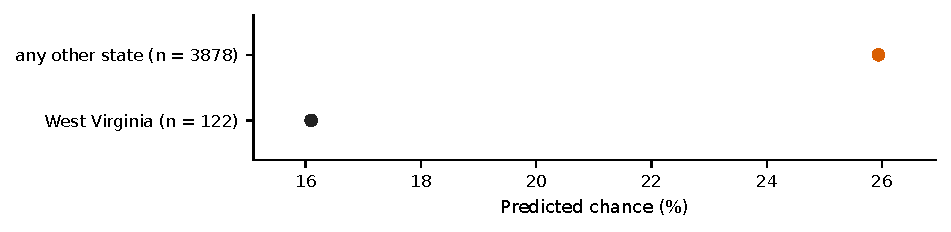
\includegraphics[width=\linewidth,height=0.88\textheight,keepaspectratio]{figures/churn100-s2-c1/ann_93-categories-small.pdf}
\caption{Many service calls: The predicted value for the typical case at each level, through this part (n = training customers; grey: fewer than 20).}
\label{fig:churn100s2c1:plot-ann93-0}
\end{figure}
\begin{figure}[H]\centering
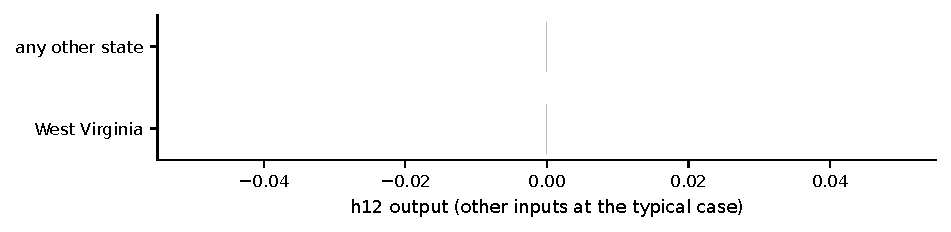
\includegraphics[width=\linewidth,height=0.88\textheight,keepaspectratio]{figures/churn100-s2-c1/ann_93-partial-7208.pdf}
\caption{Many service calls: This part's own output, unit h12 (the output of 'Many service calls'), on its own scale (its activation), with every other input at the typical case; it is active for 306 of 4000. Its output for each combination of the levels it reads.}
\label{fig:churn100s2c1:plot-ann93-1}
\end{figure}
\begin{figure}[H]\centering
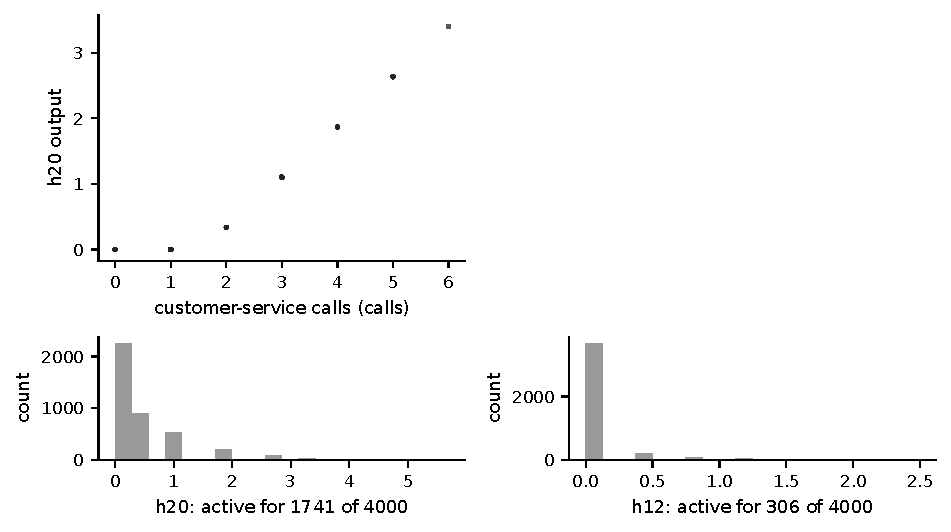
\includegraphics[width=\linewidth,height=0.88\textheight,keepaspectratio]{figures/churn100-s2-c1/ann_93-units.pdf}
\caption{Many service calls: This part's hidden units: each unit's output against its main numeric input (top) and how often it is active (bottom).}
\label{fig:churn100s2c1:plot-ann93-2}
\end{figure}
\par\smallskip\noindent{\small Technical detail: \ref{tech:ann93}.\par}
\subsubsection{Voice-mail discount}\label{rd:ann95}
\noindent{\footnotesize Part of: The whole model (\ref{rd:ann102}).\par}
\noindent{\small Figure~\ref{fig:churn100s2c1:parts-ann95} shows what feeds this part; Figure~\ref{fig:churn100s2c1:units-ann95} its units and every connection into them (dashed boxes: connections from or to other parts, drawn in their own sections).\par}
\begin{figure}[H]\centering
\resizebox{!}{\ifdim\height>0.5\textheight 0.5\textheight\else\height\fi}{%
\resizebox{\ifdim\width>\linewidth\linewidth\else\width\fi}{!}{%
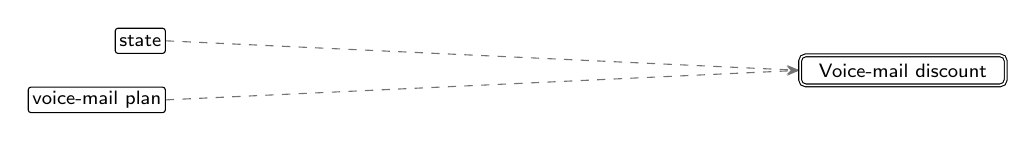
\begin{tikzpicture}[
  font=\sffamily\scriptsize, >={Stealth[length=1.6mm]},
  inp/.style={draw, rounded corners=1pt, fill=white, inner sep=1.5pt, minimum height=3.2mm, anchor=east},
  abox/.style={draw, thick, rounded corners=2pt, align=center, inner sep=3pt, minimum height=6mm, text width=42mm},
  outp/.style={draw, double, rounded corners=2pt, fill=white, align=center, inner sep=3pt, text width=24mm},
  agg/.style={draw=black!55},
]
\node[inp] (i0) at (0,0.375) {state};
\node[inp] (i1) at (0,-0.375) {voice-mail plan};
\node[outp] (out) at (9.36,0) {Voice-mail discount};
\begin{scope}[on background layer]
\draw[->, agg, thin, dashed] (i0.east) -- (out.west);
\draw[->, agg, thin, dashed] (i1.east) -- (out.west);
\end{scope}
\end{tikzpicture}}}%
\caption{Voice-mail discount: what feeds it, one level down.}
\label{fig:churn100s2c1:parts-ann95}
\end{figure}
\begin{figure}[H]\centering
\resizebox{\ifdim\width>\linewidth\linewidth\else\width\fi}{!}{%
\definecolor{netup}{HTML}{D95F02}\definecolor{netdown}{HTML}{1B9E77}\definecolor{netmixed}{HTML}{7F7F7F}%
\begin{tikzpicture}[
  font=\sffamily\scriptsize, >={Stealth[length=1.4mm]},
  inp/.style={draw, circle, fill=white, minimum size=3.2mm, inner sep=0pt},
  hid/.style={draw, circle, fill=white, minimum size=5.2mm, inner sep=0.5pt, font=\sffamily\tiny},
  exitbox/.style={draw, thick, rectangle, fill=white, align=center, text width=17mm, minimum height=5mm, inner sep=1.5pt, font=\sffamily\tiny},
  sumbox/.style={draw, thick, dashed, rectangle, fill=white, align=center, text width=17mm, minimum height=5mm, inner sep=1.5pt, font=\sffamily\tiny},
  outp/.style={draw, thick, regular polygon, regular polygon sides=6, fill=white, minimum size=10mm, inner sep=0pt, font=\sffamily\tiny, align=center},
  stub/.style={draw, dashed, rounded corners=2pt, fill=white, align=center, inner sep=2pt, font=\sffamily\tiny, text width=15mm},
  inlab/.style={font=\sffamily\tiny, align=center, text width=15mm, inner sep=1pt, fill=white, fill opacity=0.8, text opacity=1},
  wpos/.style={draw=NavyBlue}, wneg/.style={draw=BrickRed}, wagg/.style={draw=black!45, line width=1.2pt},
  wmix/.style={draw=Plum},
]
\node[hid] (n1133) at (1.9,3.25) {h5};
\node[hid] (n4051) at (1.9,4.6) {h9};
\node[hid] (n5577) at (1.9,1.9) {h10};
\node[inp, draw=netmixed, very thick] (ngrpxxstate) at (1.0,0.0) {};
\path (ngrpxxstate.south) node[inlab, anchor=north] (labngrpxxstate) {state (31 of 51 used) $\updownarrow$};
\node[inp, draw=netdown, very thick] (ninxxvoicexmailxplan) at (2.8,0.0) {};
\path (ninxxvoicexmailxplan.south) node[inlab, anchor=north] (labninxxvoicexmailxplan) {a voice-mail plan $\downarrow$};
\node[stub] (ntoxxthexmodelxoutput) at (1.9,6.15) {to the model output};
\begin{scope}[on background layer]
\node[fit=(n1133) (n4051) (n5577) , inner sep=8pt, rounded corners=5pt, fill=Orchid!10, draw=Orchid!45] (clu0) {};
\draw[->, wpos, line width=0.65pt] (n1133) -- (n4051);
\draw[->, wpos, line width=0.30pt] (n5577) -- (n1133);
\draw[->, wpos, line width=0.60pt] (ninxxvoicexmailxplan) -- (n5577);
\draw[->, wneg, line width=0.58pt] (n1133) -- (ntoxxthexmodelxoutput);
\draw[->, wneg, line width=0.60pt] (n4051) -- (ntoxxthexmodelxoutput);
\draw[->, wpos, line width=0.34pt] (ngrpxxstate) -- node[pos=0.8, sloped, above, font=\sffamily\tiny, inner sep=1pt, fill=white, fill opacity=0.8, text opacity=1] {+0.26} (n5577);
\draw[->, wpos, line width=0.27pt] (ngrpxxstate) -- node[pos=0.8, sloped, above, font=\sffamily\tiny, inner sep=1pt, fill=white, fill opacity=0.8, text opacity=1] {+0.06} (n4051);
\draw[->, wpos, line width=0.26pt] (ngrpxxstate) -- node[pos=0.8, sloped, above, font=\sffamily\tiny, inner sep=1pt, fill=white, fill opacity=0.8, text opacity=1] {+0.02} (n1133);
\end{scope}
\node[font=\sffamily\scriptsize\bfseries, text=Orchid!55!black, anchor=south west, inner sep=1pt, fill=white, fill opacity=0.85, text opacity=1] at (clu0.north west) {Voice-mail discount};
\end{tikzpicture}}%
\caption{Voice-mail discount: its units and every connection into them. Blue: positive weight (raises the score); red: negative weight (lowers it); thicker: larger weight. Orange outline and up arrow: raises the final prediction; teal and down arrow: lowers it; grey and double arrow: depends.}
\label{fig:churn100s2c1:units-ann95}
\end{figure}
\paragraph{Hypothesis.} This part gives customers with a voice-mail plan a small discount on the chance of leaving.\,{\scriptsize\textcolor{NavyBlue}{[C125]}}
\paragraph{Evidence.} Through it, a voice-mail plan lowers a typical customer's chance by less than a point, and customers in states other than Alabama, North Carolina and West Virginia get about 2\% instead of about 1\%.\,{\scriptsize\textcolor{NavyBlue}{[C125, C126]}} Its formula reproduces the part exactly on all 4000 training customers.\,{\scriptsize\textcolor{NavyBlue}{[C129]}}
\par\noindent{\small Evidence plots: Figure~\ref{fig:churn100s2c1:plot-ann95-0}, Figure~\ref{fig:churn100s2c1:plot-ann95-1}.\par}
\begin{figure}[H]\centering
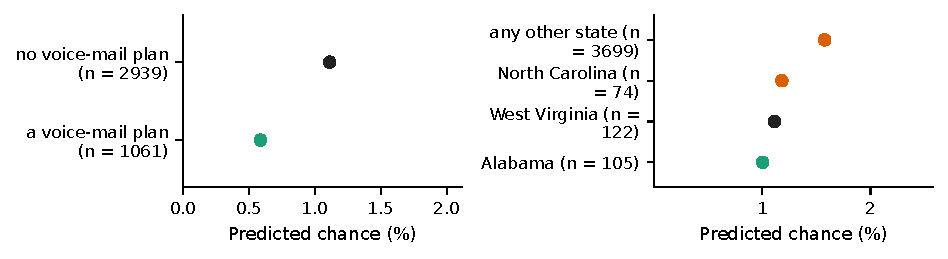
\includegraphics[width=\linewidth,height=0.88\textheight,keepaspectratio]{figures/churn100-s2-c1/ann_95-categories-small.pdf}
\caption{Voice-mail discount: The predicted value for the typical case at each level, through this part (n = training customers; grey: fewer than 20).}
\label{fig:churn100s2c1:plot-ann95-0}
\end{figure}
\begin{figure}[H]\centering
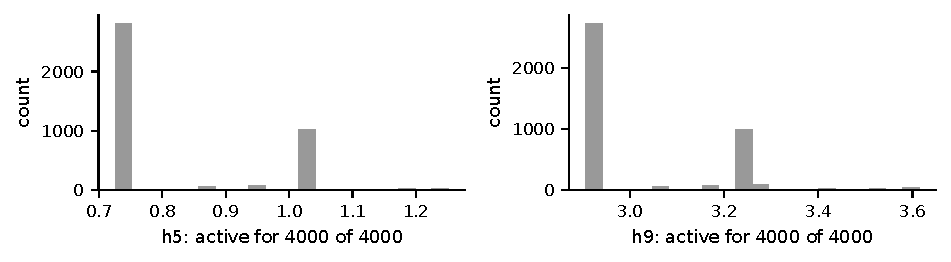
\includegraphics[width=\linewidth,height=0.88\textheight,keepaspectratio]{figures/churn100-s2-c1/ann_95-units.pdf}
\caption{Voice-mail discount: This part's hidden units: each unit's output against its main numeric input (top) and how often it is active (bottom).}
\label{fig:churn100s2c1:plot-ann95-1}
\end{figure}
\par\smallskip\noindent{\small Technical detail: \ref{tech:ann95}.\par}
\subsubsection{Heavy evening use}\label{rd:ann94}
\noindent{\footnotesize Part of: The whole model (\ref{rd:ann102}).\par}
\noindent{\small Figure~\ref{fig:churn100s2c1:parts-ann94} shows what feeds this part; Figure~\ref{fig:churn100s2c1:units-ann94} its units and every connection into them (dashed boxes: connections from or to other parts, drawn in their own sections).\par}
\begin{figure}[H]\centering
\resizebox{!}{\ifdim\height>0.5\textheight 0.5\textheight\else\height\fi}{%
\resizebox{\ifdim\width>\linewidth\linewidth\else\width\fi}{!}{%
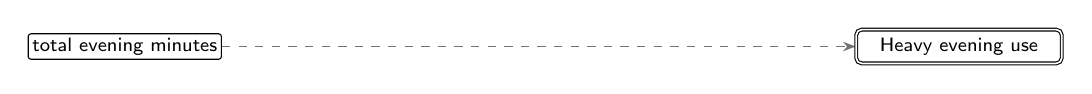
\begin{tikzpicture}[
  font=\sffamily\scriptsize, >={Stealth[length=1.6mm]},
  inp/.style={draw, rounded corners=1pt, fill=white, inner sep=1.5pt, minimum height=3.2mm, anchor=east},
  abox/.style={draw, thick, rounded corners=2pt, align=center, inner sep=3pt, minimum height=6mm, text width=42mm},
  outp/.style={draw, double, rounded corners=2pt, fill=white, align=center, inner sep=3pt, text width=24mm},
  agg/.style={draw=black!55},
]
\node[inp] (i0) at (0,-0.0) {total evening minutes};
\node[outp] (out) at (9.36,0) {Heavy evening use};
\begin{scope}[on background layer]
\draw[->, agg, thin, dashed] (i0.east) -- (out.west);
\end{scope}
\end{tikzpicture}}}%
\caption{Heavy evening use: what feeds it, one level down.}
\label{fig:churn100s2c1:parts-ann94}
\end{figure}
\begin{figure}[H]\centering
\resizebox{\ifdim\width>\linewidth\linewidth\else\width\fi}{!}{%
\definecolor{netup}{HTML}{D95F02}\definecolor{netdown}{HTML}{1B9E77}\definecolor{netmixed}{HTML}{7F7F7F}%
\begin{tikzpicture}[
  font=\sffamily\scriptsize, >={Stealth[length=1.4mm]},
  inp/.style={draw, circle, fill=white, minimum size=3.2mm, inner sep=0pt},
  hid/.style={draw, circle, fill=white, minimum size=5.2mm, inner sep=0.5pt, font=\sffamily\tiny},
  exitbox/.style={draw, thick, rectangle, fill=white, align=center, text width=17mm, minimum height=5mm, inner sep=1.5pt, font=\sffamily\tiny},
  sumbox/.style={draw, thick, dashed, rectangle, fill=white, align=center, text width=17mm, minimum height=5mm, inner sep=1.5pt, font=\sffamily\tiny},
  outp/.style={draw, thick, regular polygon, regular polygon sides=6, fill=white, minimum size=10mm, inner sep=0pt, font=\sffamily\tiny, align=center},
  stub/.style={draw, dashed, rounded corners=2pt, fill=white, align=center, inner sep=2pt, font=\sffamily\tiny, text width=15mm},
  inlab/.style={font=\sffamily\tiny, align=center, text width=15mm, inner sep=1pt, fill=white, fill opacity=0.8, text opacity=1},
  wpos/.style={draw=NavyBlue}, wneg/.style={draw=BrickRed}, wagg/.style={draw=black!45, line width=1.2pt},
  wmix/.style={draw=Plum},
]
\node[exitbox] (n476) at (1.7,1.9) {Heavy evening use $\downarrow$};
\node[inp, draw=netdown, very thick] (ninxxtotalxevexminutes) at (1.7,0.0) {};
\path (ninxxtotalxevexminutes.south) node[inlab, anchor=north] (labninxxtotalxevexminutes) {total evening minutes $\downarrow$};
\node[stub] (ntoxxthexmodelxoutput) at (1.7,3.45) {to the model output};
\begin{scope}[on background layer]
\node[fit=(n476) , inner sep=8pt, rounded corners=5pt, fill=Goldenrod!10, draw=Goldenrod!45] (clu0) {};
\draw[->, wpos, line width=0.63pt] (ninxxtotalxevexminutes) -- (n476);
\draw[->, wneg, line width=0.44pt] (n476) -- (ntoxxthexmodelxoutput);
\end{scope}
\node[font=\sffamily\scriptsize\bfseries, text=Goldenrod!55!black, anchor=south west, inner sep=1pt, fill=white, fill opacity=0.85, text opacity=1] at (clu0.north west) {Heavy evening use};
\end{tikzpicture}}%
\caption{Heavy evening use: its units and every connection into them. Blue: positive weight (raises the score); red: negative weight (lowers it); thicker: larger weight. Orange outline and up arrow: raises the final prediction; teal and down arrow: lowers it; grey and double arrow: depends.}
\label{fig:churn100s2c1:units-ann94}
\end{figure}
\paragraph{Hypothesis.} This part lowers the chance of leaving a little for customers with heavy evening use: evening minutes add nothing until about 239 minutes, then lower it steadily.\,{\scriptsize\textcolor{NavyBlue}{[C134]}}
\paragraph{Evidence.} It acts on 885 of 4000 training customers, 165 of whom left; for the typical customer it acts on, the chance is about 5\% without it and about 4\% with it.\,{\scriptsize\textcolor{NavyBlue}{[C136]}} Through it, evening minutes change nothing until about 239 minutes, then lower a typical customer's chance steadily, from about 1\% at 138 minutes to under 1\% at 266 minutes.\,{\scriptsize\textcolor{NavyBlue}{[C134]}} Its formula reproduces the part exactly on all 4000 training customers.\,{\scriptsize\textcolor{NavyBlue}{[C137]}}
\par\noindent{\small Evidence plots: Figure~\ref{fig:churn100s2c1:plot-ann94-0}, Figure~\ref{fig:churn100s2c1:plot-ann94-1}, Figure~\ref{fig:churn100s2c1:plot-ann94-2}.\par}
\par\noindent{\small Figure~\ref{fig:churn100s2c1:plot-ann94-1} shows this part's own output, unit h3: it switches on at about 238.8 minutes of total evening minutes, and is zero below.\par}
\begin{figure}[H]\centering
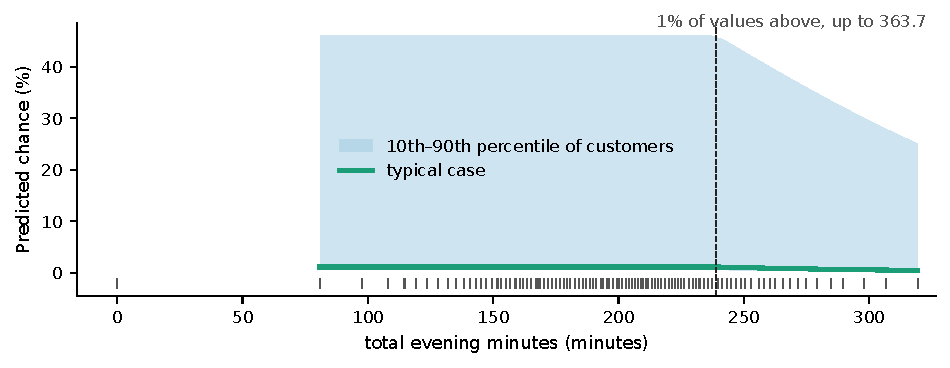
\includegraphics[width=\linewidth,height=0.88\textheight,keepaspectratio]{figures/churn100-s2-c1/ann_94-response.pdf}
\caption{Heavy evening use: Response curves through this part: the typical case (bold), the 10th to 90th percentile of individual customers (band), the fold or step point (dashed) with its spread across them (grey), and the observed values (ticks).}
\label{fig:churn100s2c1:plot-ann94-0}
\end{figure}
\begin{figure}[H]\centering
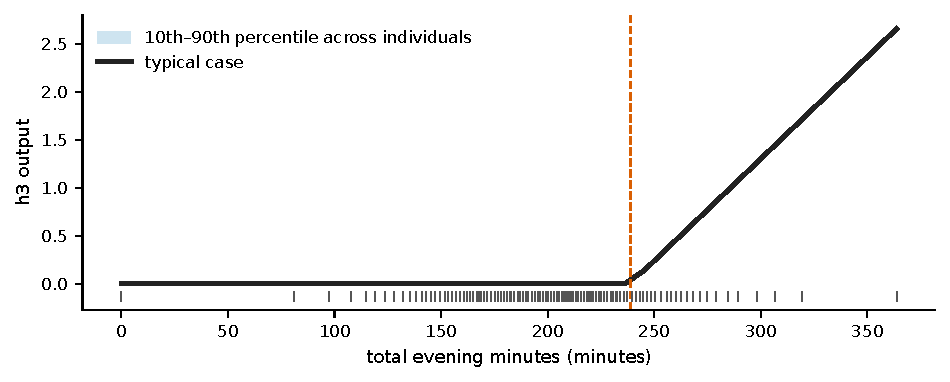
\includegraphics[width=\linewidth,height=0.88\textheight,keepaspectratio]{figures/churn100-s2-c1/ann_94-partial-476.pdf}
\caption{Heavy evening use: This part's own output, unit h3 (the output of 'Heavy evening use'), on its own scale (its activation), with every other input at the typical case; it is active for 885 of 4000. Bold: the typical case; band: 10th to 90th percentile across individuals; dashed: where it switches on; ticks: the data.}
\label{fig:churn100s2c1:plot-ann94-1}
\end{figure}
\begin{figure}[H]\centering
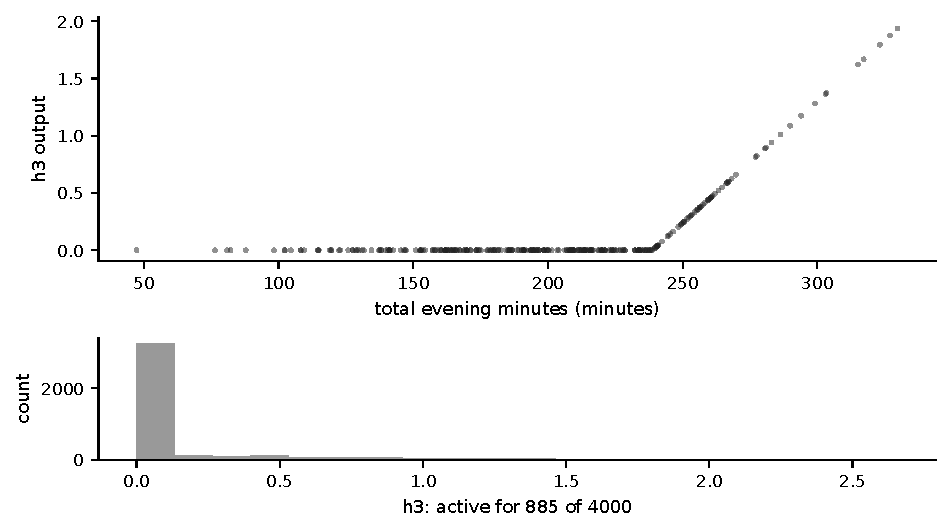
\includegraphics[width=\linewidth,height=0.88\textheight,keepaspectratio]{figures/churn100-s2-c1/ann_94-units.pdf}
\caption{Heavy evening use: This part's hidden units: each unit's output against its main numeric input (top) and how often it is active (bottom).}
\label{fig:churn100s2c1:plot-ann94-2}
\end{figure}
\par\smallskip\noindent{\small Technical detail: \ref{tech:ann94}.\par}
\subsubsection{State units}\label{rd:ann96}
\noindent{\footnotesize Part of: The whole model (\ref{rd:ann102}).\par}
\noindent{\small Figure~\ref{fig:churn100s2c1:parts-ann96} shows what feeds this part; Figure~\ref{fig:churn100s2c1:units-ann96} its units and every connection into them (dashed boxes: connections from or to other parts, drawn in their own sections).\par}
\begin{figure}[H]\centering
\resizebox{!}{\ifdim\height>0.5\textheight 0.5\textheight\else\height\fi}{%
\resizebox{\ifdim\width>\linewidth\linewidth\else\width\fi}{!}{%
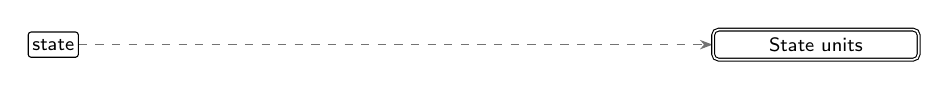
\begin{tikzpicture}[
  font=\sffamily\scriptsize, >={Stealth[length=1.6mm]},
  inp/.style={draw, rounded corners=1pt, fill=white, inner sep=1.5pt, minimum height=3.2mm, anchor=east},
  abox/.style={draw, thick, rounded corners=2pt, align=center, inner sep=3pt, minimum height=6mm, text width=42mm},
  outp/.style={draw, double, rounded corners=2pt, fill=white, align=center, inner sep=3pt, text width=24mm},
  agg/.style={draw=black!55},
]
\node[inp] (i0) at (0,-0.0) {state};
\node[outp] (out) at (9.36,0) {State units};
\begin{scope}[on background layer]
\draw[->, agg, thin, dashed] (i0.east) -- (out.west);
\end{scope}
\end{tikzpicture}}}%
\caption{State units: what feeds it, one level down.}
\label{fig:churn100s2c1:parts-ann96}
\end{figure}
\begin{figure}[H]\centering
\resizebox{\ifdim\width>\linewidth\linewidth\else\width\fi}{!}{%
\definecolor{netup}{HTML}{D95F02}\definecolor{netdown}{HTML}{1B9E77}\definecolor{netmixed}{HTML}{7F7F7F}%
\begin{tikzpicture}[
  font=\sffamily\scriptsize, >={Stealth[length=1.4mm]},
  inp/.style={draw, circle, fill=white, minimum size=3.2mm, inner sep=0pt},
  hid/.style={draw, circle, fill=white, minimum size=5.2mm, inner sep=0.5pt, font=\sffamily\tiny},
  exitbox/.style={draw, thick, rectangle, fill=white, align=center, text width=17mm, minimum height=5mm, inner sep=1.5pt, font=\sffamily\tiny},
  sumbox/.style={draw, thick, dashed, rectangle, fill=white, align=center, text width=17mm, minimum height=5mm, inner sep=1.5pt, font=\sffamily\tiny},
  outp/.style={draw, thick, regular polygon, regular polygon sides=6, fill=white, minimum size=10mm, inner sep=0pt, font=\sffamily\tiny, align=center},
  stub/.style={draw, dashed, rounded corners=2pt, fill=white, align=center, inner sep=2pt, font=\sffamily\tiny, text width=15mm},
  inlab/.style={font=\sffamily\tiny, align=center, text width=15mm, inner sep=1pt, fill=white, fill opacity=0.8, text opacity=1},
  wpos/.style={draw=NavyBlue}, wneg/.style={draw=BrickRed}, wagg/.style={draw=black!45, line width=1.2pt},
  wmix/.style={draw=Plum},
]
\node[hid] (n13827) at (3.35,4.6) {h18};
\node[hid] (n11951) at (1.85,1.9) {h16};
\node[hid] (n3861) at (4.85,1.9) {h8};
\node[hid] (n6730) at (3.35,3.25) {h11};
\node[hid] (n10249) at (0.35,1.9) {h14};
\node[hid] (n14942) at (3.35,1.9) {h19};
\node[hid] (n8896) at (6.35,1.9) {h13};
\node[inp, draw=netmixed, very thick] (ngrpxxstate) at (3.35,0.0) {};
\path (ngrpxxstate.south) node[inlab, anchor=north] (labngrpxxstate) {state (31 of 51 used) $\updownarrow$};
\node[stub] (ntoxxthexmodelxoutput) at (3.35,6.15) {to the model output};
\begin{scope}[on background layer]
\node[fit=(n13827) (n11951) (n3861) (n6730) (n10249) (n14942) (n8896) , inner sep=8pt, rounded corners=5pt, fill=Cerulean!10, draw=Cerulean!45] (clu0) {};
\draw[->, wneg, line width=0.25pt] (n11951) -- (n6730);
\draw[->, wpos, line width=0.60pt] (n6730) -- (n13827);
\draw[->, wneg, line width=0.30pt] (n3861) -- (ntoxxthexmodelxoutput);
\draw[->, wpos, line width=0.26pt] (n8896) -- (ntoxxthexmodelxoutput);
\draw[->, wpos, line width=0.26pt] (n10249) -- (ntoxxthexmodelxoutput);
\draw[->, wpos, line width=0.40pt] (n13827) -- (ntoxxthexmodelxoutput);
\draw[->, wpos, line width=0.26pt] (n14942) -- (ntoxxthexmodelxoutput);
\draw[->, wneg, line width=0.60pt] (ngrpxxstate) -- node[pos=0.8, sloped, above, font=\sffamily\tiny, inner sep=1pt, fill=white, fill opacity=0.8, text opacity=1] {-1.00} (n8896);
\draw[->, wmix, line width=0.40pt] (ngrpxxstate) -- node[pos=0.8, sloped, above, font=\sffamily\tiny, inner sep=1pt, fill=white, fill opacity=0.8, text opacity=1] {3 edges, -0.42 to +0.00} (n6730);
\draw[->, wneg, line width=0.52pt] (ngrpxxstate) -- node[pos=0.8, sloped, above, font=\sffamily\tiny, inner sep=1pt, fill=white, fill opacity=0.8, text opacity=1] {-0.77} (n3861);
\draw[->, wpos, line width=0.60pt] (ngrpxxstate) -- node[pos=0.8, sloped, above, font=\sffamily\tiny, inner sep=1pt, fill=white, fill opacity=0.8, text opacity=1] {+1.00} (n10249);
\draw[->, wpos, line width=0.60pt] (ngrpxxstate) -- node[pos=0.8, sloped, above, font=\sffamily\tiny, inner sep=1pt, fill=white, fill opacity=0.8, text opacity=1] {+1.00} (n11951);
\draw[->, wpos, line width=0.60pt] (ngrpxxstate) -- node[pos=0.8, sloped, above, font=\sffamily\tiny, inner sep=1pt, fill=white, fill opacity=0.8, text opacity=1] {+1.00} (n14942);
\end{scope}
\node[font=\sffamily\scriptsize\bfseries, text=Cerulean!55!black, anchor=south west, inner sep=1pt, fill=white, fill opacity=0.85, text opacity=1] at (clu0.north west) {State units};
\end{tikzpicture}}%
\caption{State units: its units and every connection into them. Blue: positive weight (raises the score); red: negative weight (lowers it); thicker: larger weight. Orange outline and up arrow: raises the final prediction; teal and down arrow: lowers it; grey and double arrow: depends.}
\label{fig:churn100s2c1:units-ann96}
\end{figure}
\paragraph{Hypothesis.} This part adds small state offsets: up in Arizona and Ohio, down in Nevada.\,{\scriptsize\textcolor{NavyBlue}{[C138, C139, C140]}}
\paragraph{Evidence.} Through it, a typical customer's chance moves by less than half a point: up in Arizona and Ohio, down in Nevada, with Missouri and Massachusetts almost unchanged.\,{\scriptsize\textcolor{NavyBlue}{[C138, C139, C140, C141, C142]}} Its formula reproduces the part exactly on all 4000 training customers.\,{\scriptsize\textcolor{NavyBlue}{[C143]}}
\par\noindent{\small Evidence plots: Figure~\ref{fig:churn100s2c1:plot-ann96-0}, Figure~\ref{fig:churn100s2c1:plot-ann96-1}.\par}
\begin{figure}[H]\centering
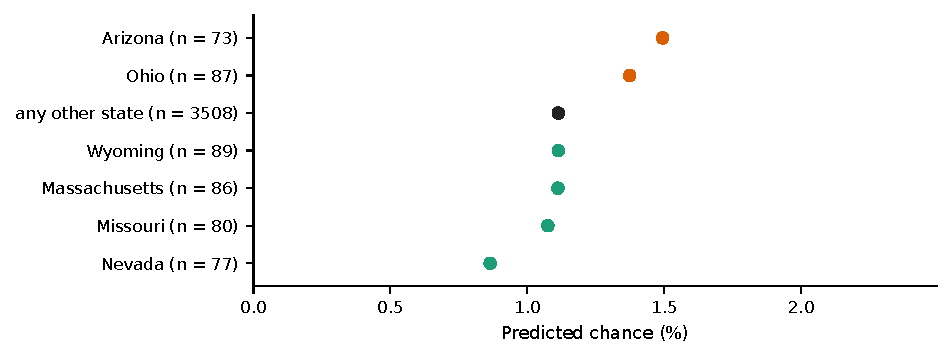
\includegraphics[width=\linewidth,height=0.88\textheight,keepaspectratio]{figures/churn100-s2-c1/ann_96-categories-C138.pdf}
\caption{State units: The predicted value for the typical case at each level, through this part (n = training customers; grey: fewer than 20).}
\label{fig:churn100s2c1:plot-ann96-0}
\end{figure}
\begin{figure}[H]\centering
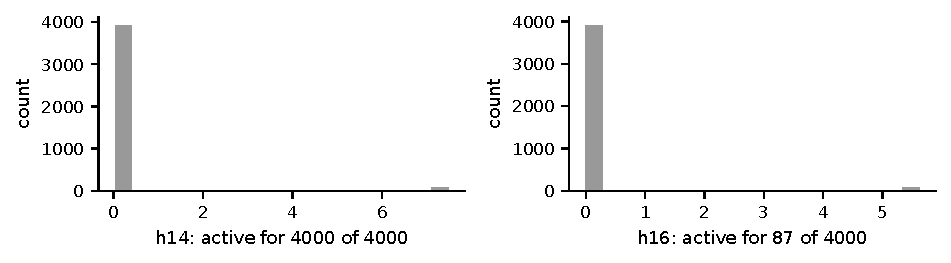
\includegraphics[width=\linewidth,height=0.88\textheight,keepaspectratio]{figures/churn100-s2-c1/ann_96-units.pdf}
\caption{State units: This part's hidden units: each unit's output against its main numeric input (top) and how often it is active (bottom).}
\label{fig:churn100s2c1:plot-ann96-1}
\end{figure}
\par\smallskip\noindent{\small Technical detail: \ref{tech:ann96}.\par}
\subsubsection{Daytime calls and Tennessee}\label{rd:ann97}
\noindent{\footnotesize Part of: The whole model (\ref{rd:ann102}).\par}
\noindent{\small Figure~\ref{fig:churn100s2c1:parts-ann97} shows what feeds this part; Figure~\ref{fig:churn100s2c1:units-ann97} its units and every connection into them (dashed boxes: connections from or to other parts, drawn in their own sections).\par}
\begin{figure}[H]\centering
\resizebox{!}{\ifdim\height>0.5\textheight 0.5\textheight\else\height\fi}{%
\resizebox{\ifdim\width>\linewidth\linewidth\else\width\fi}{!}{%
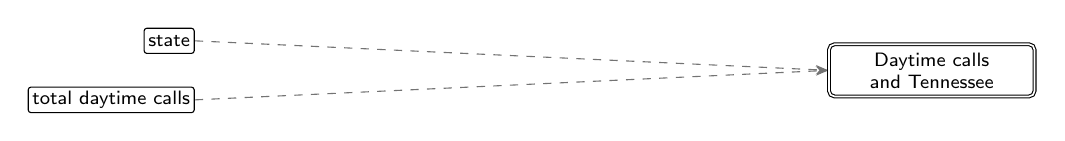
\begin{tikzpicture}[
  font=\sffamily\scriptsize, >={Stealth[length=1.6mm]},
  inp/.style={draw, rounded corners=1pt, fill=white, inner sep=1.5pt, minimum height=3.2mm, anchor=east},
  abox/.style={draw, thick, rounded corners=2pt, align=center, inner sep=3pt, minimum height=6mm, text width=42mm},
  outp/.style={draw, double, rounded corners=2pt, fill=white, align=center, inner sep=3pt, text width=24mm},
  agg/.style={draw=black!55},
]
\node[inp] (i0) at (0,0.375) {state};
\node[inp] (i1) at (0,-0.375) {total daytime calls};
\node[outp] (out) at (9.36,0) {Daytime calls and Tennessee};
\begin{scope}[on background layer]
\draw[->, agg, thin, dashed] (i0.east) -- (out.west);
\draw[->, agg, thin, dashed] (i1.east) -- (out.west);
\end{scope}
\end{tikzpicture}}}%
\caption{Daytime calls and Tennessee: what feeds it, one level down.}
\label{fig:churn100s2c1:parts-ann97}
\end{figure}
\begin{figure}[H]\centering
\resizebox{\ifdim\width>\linewidth\linewidth\else\width\fi}{!}{%
\definecolor{netup}{HTML}{D95F02}\definecolor{netdown}{HTML}{1B9E77}\definecolor{netmixed}{HTML}{7F7F7F}%
\begin{tikzpicture}[
  font=\sffamily\scriptsize, >={Stealth[length=1.4mm]},
  inp/.style={draw, circle, fill=white, minimum size=3.2mm, inner sep=0pt},
  hid/.style={draw, circle, fill=white, minimum size=5.2mm, inner sep=0.5pt, font=\sffamily\tiny},
  exitbox/.style={draw, thick, rectangle, fill=white, align=center, text width=17mm, minimum height=5mm, inner sep=1.5pt, font=\sffamily\tiny},
  sumbox/.style={draw, thick, dashed, rectangle, fill=white, align=center, text width=17mm, minimum height=5mm, inner sep=1.5pt, font=\sffamily\tiny},
  outp/.style={draw, thick, regular polygon, regular polygon sides=6, fill=white, minimum size=10mm, inner sep=0pt, font=\sffamily\tiny, align=center},
  stub/.style={draw, dashed, rounded corners=2pt, fill=white, align=center, inner sep=2pt, font=\sffamily\tiny, text width=15mm},
  inlab/.style={font=\sffamily\tiny, align=center, text width=15mm, inner sep=1pt, fill=white, fill opacity=0.8, text opacity=1},
  wpos/.style={draw=NavyBlue}, wneg/.style={draw=BrickRed}, wagg/.style={draw=black!45, line width=1.2pt},
  wmix/.style={draw=Plum},
]
\node[exitbox] (n11427) at (2.7,1.9) {Daytime calls and Tennessee $\uparrow$};
\node[inp, draw=netmixed, very thick] (ngrpxxstate) at (1.8,0.0) {};
\path (ngrpxxstate.south) node[inlab, anchor=north] (labngrpxxstate) {state (31 of 51 used) $\updownarrow$};
\node[inp, draw=netdown, very thick] (ninxxtotalxdayxcalls) at (3.6,0.0) {};
\path (ninxxtotalxdayxcalls.south) node[inlab, anchor=north] (labninxxtotalxdayxcalls) {total daytime calls $\downarrow$};
\node[stub] (ntoxxthexmodelxoutput) at (2.7,3.45) {to the model output};
\begin{scope}[on background layer]
\node[fit=(n11427) , inner sep=8pt, rounded corners=5pt, fill=Mahogany!10, draw=Mahogany!45] (clu0) {};
\draw[->, wneg, line width=0.29pt] (ninxxtotalxdayxcalls) -- (n11427);
\draw[->, wpos, line width=0.27pt] (n11427) -- (ntoxxthexmodelxoutput);
\draw[->, wpos, line width=0.60pt] (ngrpxxstate) -- node[pos=0.8, sloped, above, font=\sffamily\tiny, inner sep=1pt, fill=white, fill opacity=0.8, text opacity=1] {+1.00} (n11427);
\end{scope}
\node[font=\sffamily\scriptsize\bfseries, text=Mahogany!55!black, anchor=south west, inner sep=1pt, fill=white, fill opacity=0.85, text opacity=1] at (clu0.north west) {Daytime calls and Tennessee};
\end{tikzpicture}}%
\caption{Daytime calls and Tennessee: its units and every connection into them. Blue: positive weight (raises the score); red: negative weight (lowers it); thicker: larger weight. Orange outline and up arrow: raises the final prediction; teal and down arrow: lowers it; grey and double arrow: depends.}
\label{fig:churn100s2c1:units-ann97}
\end{figure}
\paragraph{Hypothesis.} This part gives customers in Tennessee a small rise in the chance of leaving; daytime calls barely change it.\,{\scriptsize\textcolor{NavyBlue}{[C144, C145]}}
\paragraph{Evidence.} Through it, being in Tennessee takes a typical customer's chance from about 1\% to about 2\%, and going from 75 to 125 daytime calls barely changes it.\,{\scriptsize\textcolor{NavyBlue}{[C144, C145]}} Its formula reproduces the part exactly on all 4000 training customers.\,{\scriptsize\textcolor{NavyBlue}{[C149]}}
\par\noindent{\small Evidence plots: Figure~\ref{fig:churn100s2c1:plot-ann97-0}, Figure~\ref{fig:churn100s2c1:plot-ann97-1}, Figure~\ref{fig:churn100s2c1:plot-ann97-2}, Figure~\ref{fig:churn100s2c1:plot-ann97-3}.\par}
\par\noindent{\small Figure~\ref{fig:churn100s2c1:plot-ann97-2} shows this part's own output, unit h15: it switches on at about 113 calls of total daytime calls, and is zero below.\par}
\begin{figure}[H]\centering
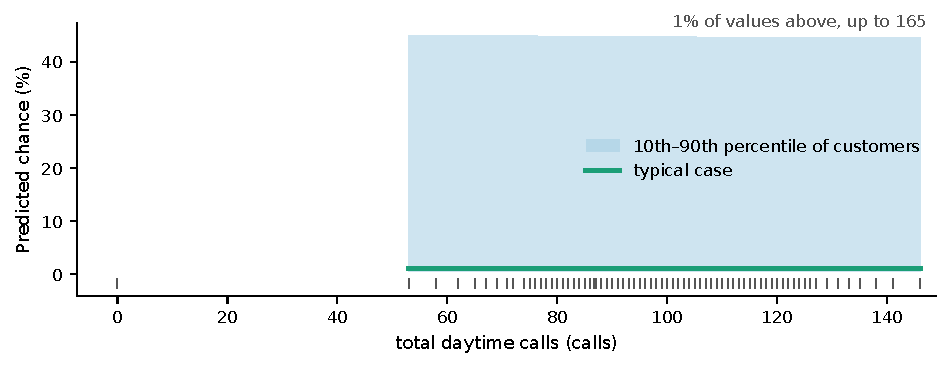
\includegraphics[width=\linewidth,height=0.88\textheight,keepaspectratio]{figures/churn100-s2-c1/ann_97-response.pdf}
\caption{Daytime calls and Tennessee: Response curves through this part: the typical case (bold), the 10th to 90th percentile of individual customers (band), the fold or step point (dashed) with its spread across them (grey), and the observed values (ticks).}
\label{fig:churn100s2c1:plot-ann97-0}
\end{figure}
\begin{figure}[H]\centering
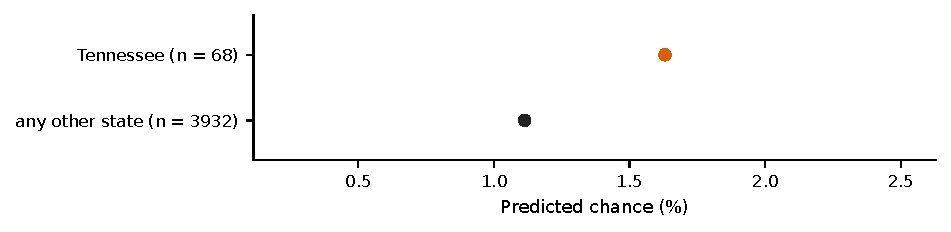
\includegraphics[width=\linewidth,height=0.88\textheight,keepaspectratio]{figures/churn100-s2-c1/ann_97-categories-small.pdf}
\caption{Daytime calls and Tennessee: The predicted value for the typical case at each level, through this part (n = training customers; grey: fewer than 20).}
\label{fig:churn100s2c1:plot-ann97-1}
\end{figure}
\begin{figure}[H]\centering
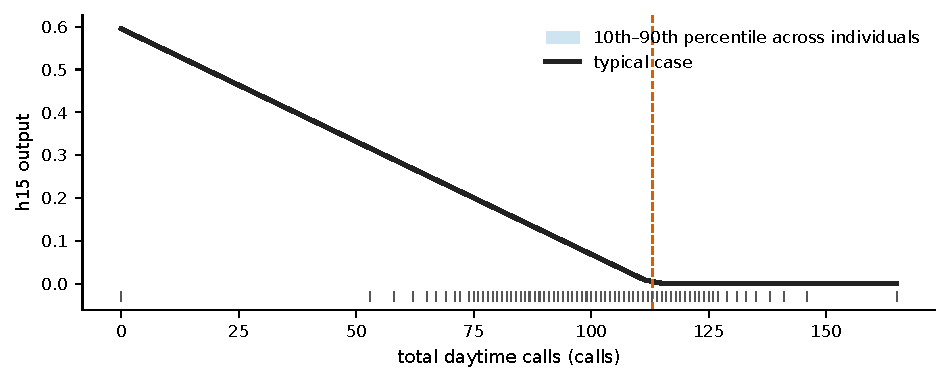
\includegraphics[width=\linewidth,height=0.88\textheight,keepaspectratio]{figures/churn100-s2-c1/ann_97-partial-11427.pdf}
\caption{Daytime calls and Tennessee: This part's own output, unit h15 (the output of 'Daytime calls and Tennessee'), on its own scale (its activation), with every other input at the typical case; it is active for 2994 of 4000. Bold: the typical case; band: 10th to 90th percentile across individuals; dashed: where it switches on; ticks: the data.}
\label{fig:churn100s2c1:plot-ann97-2}
\end{figure}
\begin{figure}[H]\centering
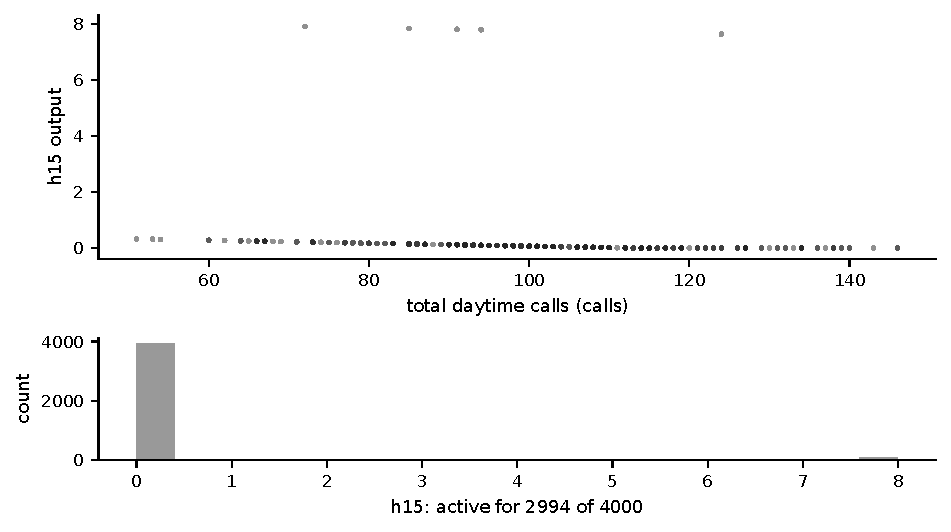
\includegraphics[width=\linewidth,height=0.88\textheight,keepaspectratio]{figures/churn100-s2-c1/ann_97-units.pdf}
\caption{Daytime calls and Tennessee: This part's hidden units: each unit's output against its main numeric input (top) and how often it is active (bottom).}
\label{fig:churn100s2c1:plot-ann97-3}
\end{figure}
\par\smallskip\noindent{\small Technical detail: \ref{tech:ann97}.\par}
\subsubsection{Small state unit}\label{rd:ann92}
\noindent{\footnotesize Part of: The whole model (\ref{rd:ann102}).\par}
\noindent{\small Figure~\ref{fig:churn100s2c1:parts-ann92} shows what feeds this part; Figure~\ref{fig:churn100s2c1:units-ann92} its units and every connection into them (dashed boxes: connections from or to other parts, drawn in their own sections).\par}
\begin{figure}[H]\centering
\resizebox{!}{\ifdim\height>0.5\textheight 0.5\textheight\else\height\fi}{%
\resizebox{\ifdim\width>\linewidth\linewidth\else\width\fi}{!}{%
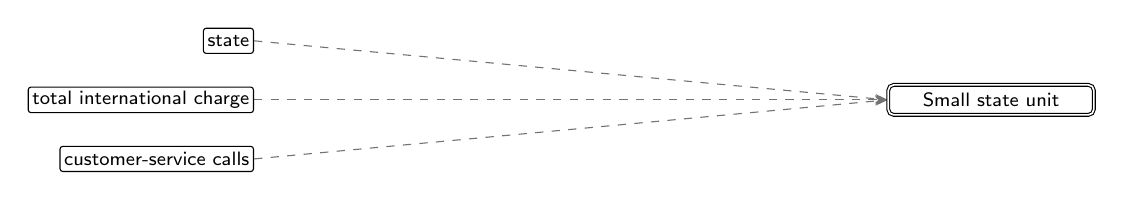
\begin{tikzpicture}[
  font=\sffamily\scriptsize, >={Stealth[length=1.6mm]},
  inp/.style={draw, rounded corners=1pt, fill=white, inner sep=1.5pt, minimum height=3.2mm, anchor=east},
  abox/.style={draw, thick, rounded corners=2pt, align=center, inner sep=3pt, minimum height=6mm, text width=42mm},
  outp/.style={draw, double, rounded corners=2pt, fill=white, align=center, inner sep=3pt, text width=24mm},
  agg/.style={draw=black!55},
]
\node[inp] (i0) at (0,0.75) {state};
\node[inp] (i1) at (0,-0.0) {total international charge};
\node[inp] (i2) at (0,-0.75) {customer-service calls};
\node[outp] (out) at (9.36,0) {Small state unit};
\begin{scope}[on background layer]
\draw[->, agg, thin, dashed] (i0.east) -- (out.west);
\draw[->, agg, thin, dashed] (i1.east) -- (out.west);
\draw[->, agg, thin, dashed] (i2.east) -- (out.west);
\end{scope}
\end{tikzpicture}}}%
\caption{Small state unit: what feeds it, one level down.}
\label{fig:churn100s2c1:parts-ann92}
\end{figure}
\begin{figure}[H]\centering
\resizebox{\ifdim\width>\linewidth\linewidth\else\width\fi}{!}{%
\definecolor{netup}{HTML}{D95F02}\definecolor{netdown}{HTML}{1B9E77}\definecolor{netmixed}{HTML}{7F7F7F}%
\begin{tikzpicture}[
  font=\sffamily\scriptsize, >={Stealth[length=1.4mm]},
  inp/.style={draw, circle, fill=white, minimum size=3.2mm, inner sep=0pt},
  hid/.style={draw, circle, fill=white, minimum size=5.2mm, inner sep=0.5pt, font=\sffamily\tiny},
  exitbox/.style={draw, thick, rectangle, fill=white, align=center, text width=17mm, minimum height=5mm, inner sep=1.5pt, font=\sffamily\tiny},
  sumbox/.style={draw, thick, dashed, rectangle, fill=white, align=center, text width=17mm, minimum height=5mm, inner sep=1.5pt, font=\sffamily\tiny},
  outp/.style={draw, thick, regular polygon, regular polygon sides=6, fill=white, minimum size=10mm, inner sep=0pt, font=\sffamily\tiny, align=center},
  stub/.style={draw, dashed, rounded corners=2pt, fill=white, align=center, inner sep=2pt, font=\sffamily\tiny, text width=15mm},
  inlab/.style={font=\sffamily\tiny, align=center, text width=15mm, inner sep=1pt, fill=white, fill opacity=0.8, text opacity=1},
  wpos/.style={draw=NavyBlue}, wneg/.style={draw=BrickRed}, wagg/.style={draw=black!45, line width=1.2pt},
  wmix/.style={draw=Plum},
]
\node[hid] (n2627xa) at (2.7,3.25) {h21};
\node[hid] (n9555xa) at (3.45,1.9) {h23};
\node[hid] (n161) at (1.95,1.9) {h1};
\node[exitbox] (n252) at (2.7,4.6) {Small state unit $\uparrow$};
\node[inp, draw=netmixed, very thick] (ngrpxxstate) at (0.9,0.0) {};
\path (ngrpxxstate.south) node[inlab, anchor=north] (labngrpxxstate) {state (31 of 51 used) $\updownarrow$};
\node[inp, draw=netdown, very thick] (ninxxtotalxintlxcharge) at (2.7,0.0) {};
\path (ninxxtotalxintlxcharge.south) node[inlab, anchor=north] (labninxxtotalxintlxcharge) {total international charge $\downarrow$};
\node[inp, draw=netdown, very thick] (ninxxnumberxcustomerxservicexcalls) at (4.5,0.0) {};
\path (ninxxnumberxcustomerxservicexcalls.south) node[inlab, anchor=north] (labninxxnumberxcustomerxservicexcalls) {customer-service calls $\downarrow$};
\node[stub] (ntoxxthexmodelxoutput) at (2.7,6.15) {to the model output};
\begin{scope}[on background layer]
\node[fit=(n2627xa) (n9555xa) (n161) (n252) , inner sep=8pt, rounded corners=5pt, fill=OliveGreen!10, draw=OliveGreen!45] (clu0) {};
\draw[->, wpos, line width=0.53pt] (n161) -- (n252);
\draw[->, wneg, line width=0.38pt] (n2627xa) -- (n252);
\draw[->, wpos, line width=0.36pt] (n9555xa) -- (n2627xa);
\draw[->, wneg, line width=0.55pt] (ninxxtotalxintlxcharge) -- (n252);
\draw[->, wpos, line width=0.35pt] (ninxxnumberxcustomerxservicexcalls) -- (n2627xa);
\draw[->, wpos, line width=0.55pt] (ninxxnumberxcustomerxservicexcalls) -- (n9555xa);
\draw[->, wpos, line width=0.26pt] (n252) -- (ntoxxthexmodelxoutput);
\draw[->, wneg, line width=0.25pt] (ngrpxxstate) -- node[pos=0.8, sloped, above, font=\sffamily\tiny, inner sep=1pt, fill=white, fill opacity=0.8, text opacity=1] {-0.01} (n161);
\draw[->, wpos, line width=0.52pt] (ngrpxxstate) -- node[pos=0.8, sloped, above, font=\sffamily\tiny, inner sep=1pt, fill=white, fill opacity=0.8, text opacity=1] {2 edges, +0.44 to +0.76} (n252);
\end{scope}
\node[font=\sffamily\scriptsize\bfseries, text=OliveGreen!55!black, anchor=south west, inner sep=1pt, fill=white, fill opacity=0.85, text opacity=1] at (clu0.north west) {Small state unit};
\end{tikzpicture}}%
\caption{Small state unit: its units and every connection into them. Blue: positive weight (raises the score); red: negative weight (lowers it); thicker: larger weight. Orange outline and up arrow: raises the final prediction; teal and down arrow: lowers it; grey and double arrow: depends.}
\label{fig:churn100s2c1:units-ann92}
\end{figure}
\paragraph{Hypothesis.} This small part barely changes the chance of leaving: it adds less than a tenth of a point in Arkansas and Utah.\,{\scriptsize\textcolor{NavyBlue}{[C150, C153]}}
\paragraph{Evidence.} Through it, the chance moves by less than a tenth of a point in Arkansas and Utah, a higher international charge lowers it steadily by even less, and customer-service calls barely move it.\,{\scriptsize\textcolor{NavyBlue}{[C150, C153, C151, C152]}} Its formula reproduces the part exactly on all 4000 training customers.\,{\scriptsize\textcolor{NavyBlue}{[C161]}}
\par\noindent{\small Evidence plots: Figure~\ref{fig:churn100s2c1:plot-ann92-0}, Figure~\ref{fig:churn100s2c1:plot-ann92-1}, Figure~\ref{fig:churn100s2c1:plot-ann92-2}, Figure~\ref{fig:churn100s2c1:plot-ann92-3}, Figure~\ref{fig:churn100s2c1:plot-ann92-4}, Figure~\ref{fig:churn100s2c1:plot-ann92-5}.\par}
\par\medskip\noindent\textbf{Worked example: reading this part.} Figure~\ref{fig:churn100s2c1:plot-ann92-2} maps the part's own output over its main inputs. In the grey region it is switched off and adds nothing; past the black line it switches on, and the colour shows how much it adds to the score. The line is the rule in the claim (C164): it switches on when total international charge plus about 0.07 $\times$ customer-service calls below about 0.50 (for customer-service calls from about 0.00 to 1.73); total international charge plus about 0.14 $\times$ customer-service calls below about 0.62 (for customer-service calls from about 1.73 to 6.04). 153 of 4000 training customers lie on the 'on' side, and 12\% of them left, against 14\% of the others: the 'on' side holds mostly hollow points, so the part picks out low-risk cases. Figure~\ref{fig:churn100s2c1:plot-ann92-3} cuts the map into slices: the hinge moves as the other input changes, which is what a tilted line means. Figure~\ref{fig:churn100s2c1:plot-ann92-4} shows what this does to the final prediction for the typical case.\par
\begin{figure}[H]\centering
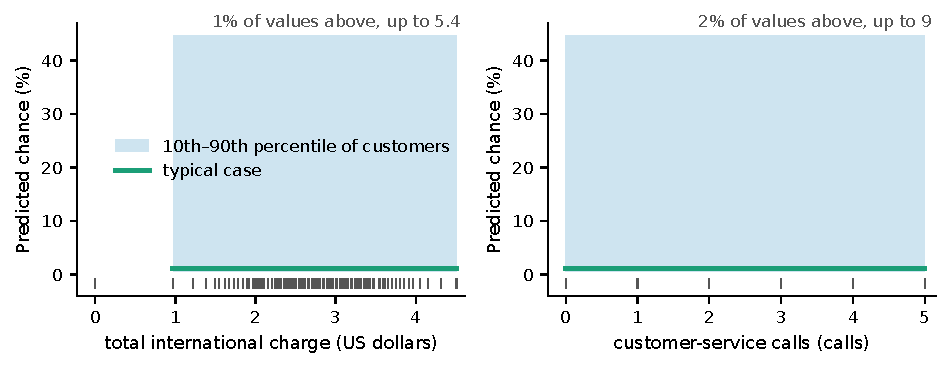
\includegraphics[width=\linewidth,height=0.88\textheight,keepaspectratio]{figures/churn100-s2-c1/ann_92-response.pdf}
\caption{Small state unit: Response curves through this part: the typical case (bold), the 10th to 90th percentile of individual customers (band), the fold or step point (dashed) with its spread across them (grey), and the observed values (ticks).}
\label{fig:churn100s2c1:plot-ann92-0}
\end{figure}
\begin{figure}[H]\centering
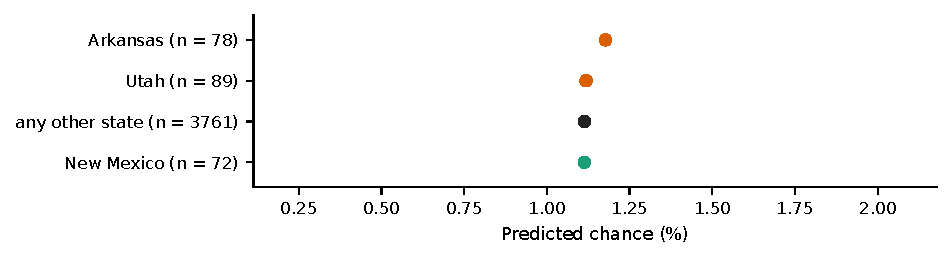
\includegraphics[width=\linewidth,height=0.88\textheight,keepaspectratio]{figures/churn100-s2-c1/ann_92-categories-small.pdf}
\caption{Small state unit: The predicted value for the typical case at each level, through this part (n = training customers; grey: fewer than 20).}
\label{fig:churn100s2c1:plot-ann92-1}
\end{figure}
\begin{figure}[H]\centering
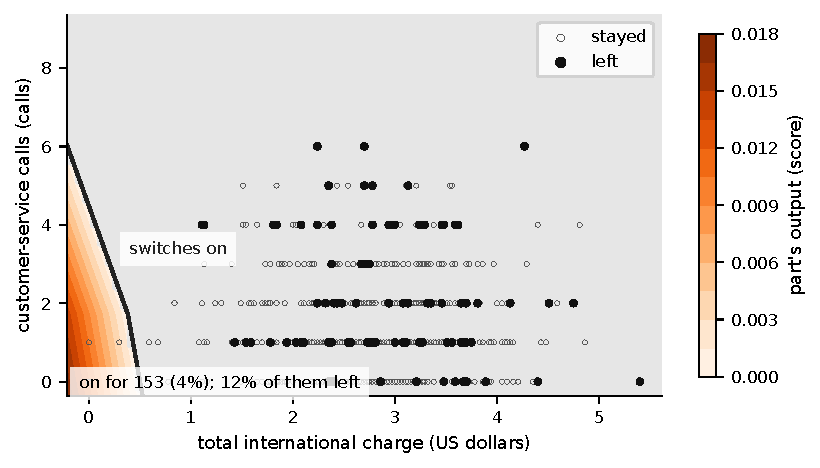
\includegraphics[width=\linewidth,height=0.88\textheight,keepaspectratio]{figures/churn100-s2-c1/ann_92-deep-map.pdf}
\caption{Small state unit: The part's own output over its two numeric inputs, other inputs at the typical case: colour where it is on, flat grey where it is switched off, the black line where it switches on; training customers as hollow (no event) and filled (event) points, so the part can be seen catching the events (the predicted-chance overlay was harder to read).}
\label{fig:churn100s2c1:plot-ann92-2}
\end{figure}
\begin{figure}[H]\centering
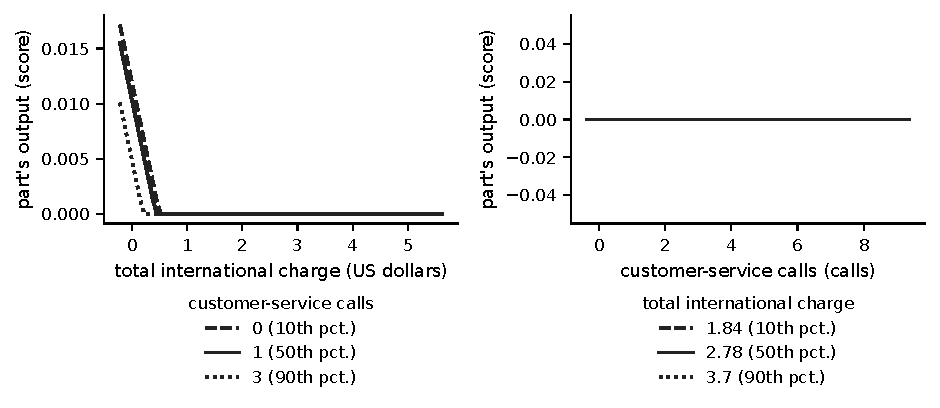
\includegraphics[width=\linewidth,height=0.88\textheight,keepaspectratio]{figures/churn100-s2-c1/ann_92-deep-slices.pdf}
\caption{Small state unit: Slices of the same map: the part's own output against each input at three values of the other, so the tilted boundary shows as a shifting hinge.}
\label{fig:churn100s2c1:plot-ann92-3}
\end{figure}
\begin{figure}[H]\centering
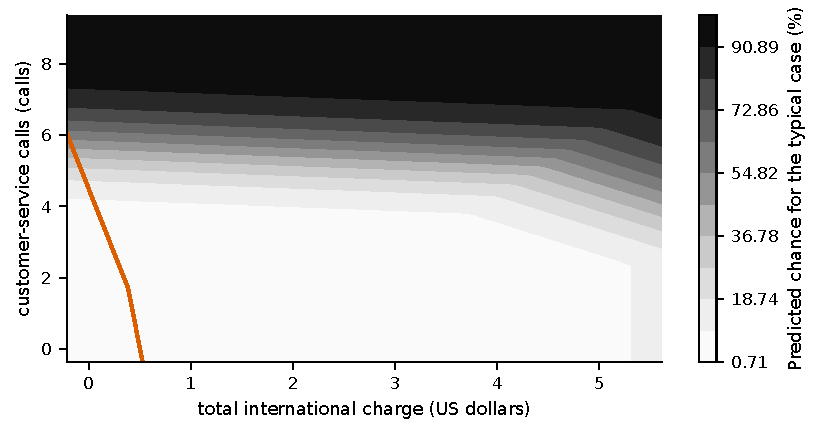
\includegraphics[width=\linewidth,height=0.88\textheight,keepaspectratio]{figures/churn100-s2-c1/ann_92-deep-risk.pdf}
\caption{Small state unit: The same map on the final scale: the predicted value for the typical case, with the switch-on line (orange).}
\label{fig:churn100s2c1:plot-ann92-4}
\end{figure}
\begin{figure}[H]\centering
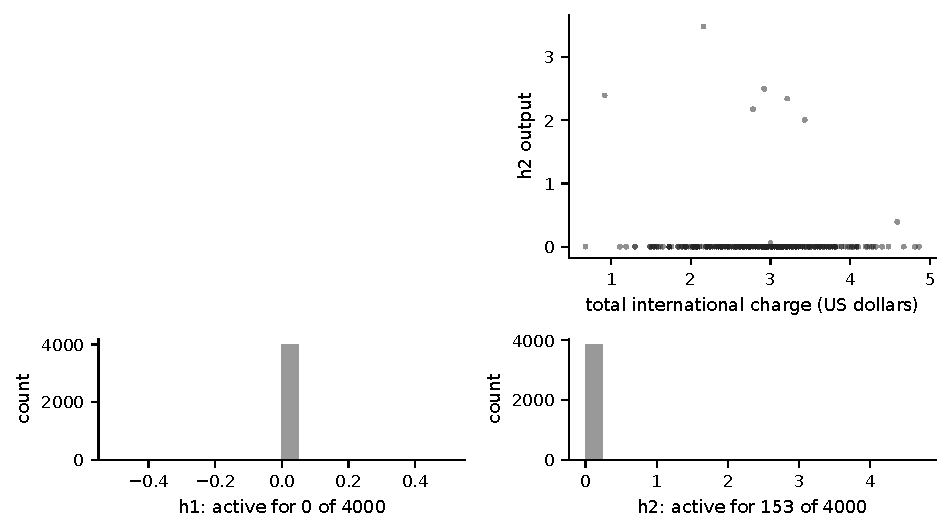
\includegraphics[width=\linewidth,height=0.88\textheight,keepaspectratio]{figures/churn100-s2-c1/ann_92-units.pdf}
\caption{Small state unit: This part's hidden units: each unit's output against its main numeric input (top) and how often it is active (bottom).}
\label{fig:churn100s2c1:plot-ann92-5}
\end{figure}
\par\smallskip\noindent{\small Technical detail: \ref{tech:ann92}.\par}
\subsection{Not supported by the model}
\begin{itemize}\setlength\itemsep{0pt}\small
\item C002: direction claim about total daytime minutes in the whole model: not supported by the model (17\% of patients have the opposite sign (allowed: 10\%)).
\item C017: direction claim about total evening charge in the whole model: not supported by the model (52\% of patients have the opposite sign (allowed: 10\%)).
\item C041: direction claim about state in the whole model: not supported by the model (45\% of patients have the opposite sign (allowed: 10\%)).
\item C044: direction claim about state in the whole model: not supported by the model (92\% of patients have the opposite sign (allowed: 10\%)).
\item C146: interaction claim about total daytime calls and state in part ann\_\allowbreak{}97: not supported by the model (the group difference is below 0.1 log-odds).
\item C147: threshold claim about total daytime calls in part ann\_\allowbreak{}97: not supported by the model (the fold changes the curve by only 0.014 log-odds compared with a straight line (needed 0.1); the effect past the fold is too small or not consistent across patients).
\item C148: subgroup claim about state and total daytime calls in part ann\_\allowbreak{}97: not supported by the model (its effect is negligible).
\item C154: interaction claim about number of calls to customer service and state in part ann\_\allowbreak{}92: not supported by the model (the part's own counterfactual difference has the opposite sign).
\item C155: interaction claim about total international charge and state in part ann\_\allowbreak{}92: not supported by the model (the group difference is below 0.1 log-odds).
\item C156: interaction claim about number of calls to customer service and total international charge in part ann\_\allowbreak{}92: not supported by the model (the group difference is below 0.1 log-odds; the part's own counterfactual difference has the opposite sign).
\item C157: threshold claim about number of calls to customer service in part ann\_\allowbreak{}92: not supported by the model (the fold changes the curve by only 0.015 log-odds compared with a straight line (needed 0.1); the effect past the fold is too small or not consistent across patients).
\item C158: threshold claim about total international charge in part ann\_\allowbreak{}92: not supported by the model (the effect past the fold is too small or not consistent across patients).
\item C159: subgroup claim about state and total international charge in part ann\_\allowbreak{}92: not supported by the model (its effect is negligible).
\item C160: null claim about state and total international charge in part ann\_\allowbreak{}92: not supported by the model (predictions move by up to 0.020).
\item C162: boundary claim about total daytime minutes and number of calls to customer service in part ann\_\allowbreak{}101: not supported by the model (no switch-on line could be traced on the first map to check against the data; no switch-on boundary in the observed range).
\item C163: boundary claim about total daytime minutes and number of calls to customer service in part ann\_\allowbreak{}91: not supported by the model (no switch-on line could be traced on the first map to check against the data; no switch-on boundary in the observed range).
\end{itemize}
\clearpage\section*{Technical detail: churn100-s2-c1}
\addcontentsline{toc}{section}{Technical detail: churn100-s2-c1}
\noindent{\small The record behind each part: the original hypothesis, the closed form, and every claim with its estimate (log-odds and odds ratio), range across patients, n and test check.\par}
\renewcommand{\thesubsection}{T.\arabic{subsection}}\setcounter{subsection}{0}
\subsection{The whole model}\label{tech:ann102}
\noindent{\footnotesize Annotation ann\_\allowbreak{}102 (churn\_\allowbreak{}logit). Reads: state, account length, area code, international calling plan, voice-mail plan, number of voice-mail messages, total daytime minutes, total daytime calls, total daytime charge, total evening minutes, total evening calls, total evening charge, total night-time minutes, total night-time calls, total night-time charge, total international minutes, total international calls, total international charge, number of calls to customer service.\par}
\paragraph{Original hypothesis (unchanged).} Root: logit P(churn) = -1.05 + linear\_\allowbreak{}backbone + service\_\allowbreak{}call\_\allowbreak{}nonlinear (identity\_\allowbreak{}svc = 1.60*807 + 1.81*1264 + 1.48*7208) - 0.95*1133 - 0.99*4051 (voicemail\_\allowbreak{}chain) - 0.55*476 (eve\_\allowbreak{}minutes\_\allowbreak{}hinge) + state\_\allowbreak{}offsets + 0.02*252 + 0.05*11427, purely additive in the logit; the sigmoid is the only coupling. 24 inputs are unconnected (total intl calls, night charge, evening calls, day charge and 20 state indicators) and have zero effect. Train AUC 0.901, accuracy 0.901. Performance sources (train): all children replaced by least-squares linear fits gives AUC 0.837 (an L2 logistic regression refit on all 71 inputs gets 0.843); restoring csc\_\allowbreak{}usage\_\allowbreak{}gate alone gives 0.898, csc\_\allowbreak{}hinge alone 0.851, eve\_\allowbreak{}minutes\_\allowbreak{}hinge alone 0.834, the others 0.837 (exactly or nearly linear). So the gain over linear comes from the service-call x low-usage gate. Rare-category switches: state:11/46/5 offsets of -2.24/-1.89/-1.46 logit on 73-80 customers (empirical -1.35/-0.91/-0.51); state:4 +1.35 (41 rows, empirical +0.80); state:47 +1.16 (72 rows, +0.92); state:49 -0.42 offset, down to -2.87 for 12 customers with 4+ calls (turns off the 4+-calls hinge); state:35 +0.40 (empirical +0.06).
\paragraph{Closed form.} Read through its parts (their formulas are in their own sections).
\paragraph{Split inputs.} To annotate the parts, the explanation split these inputs into copies (a refactoring step that does not change what the model computes); the diagrams draw each input once: customer-service calls (3 copies); total daytime calls (2 copies); total daytime minutes (2 copies); total evening charge (2 copies); total evening minutes (2 copies); total international charge (3 copies); a voice-mail plan (2 copies).
\paragraph{State: every level the model reads.} Whole-model change in the predicted chance for a typical customer when only the state changes from the reference; n = training customers in that level.\par\smallskip
{\scriptsize\rowcolors{2}{black!6}{white}
\begin{longtable}{@{}lllrlc@{}}
\toprule\rowcolor{white}
Claim & From & To & n & Chance & OK \\
\midrule\endhead
\bottomrule\endfoot
C003 & West Virginia & California & 41 & 1\% to 6\% & \textcolor{OliveGreen}{yes} \\
C004 & West Virginia & Washington & 72 & 1\% to 5\% & \textcolor{OliveGreen}{yes} \\
C006 & West Virginia & Montana & 75 & 1\% to 3\% & \textcolor{OliveGreen}{yes} \\
C007 & West Virginia & Maryland & 82 & 1\% to 3\% & \textcolor{OliveGreen}{yes} \\
C009 & West Virginia & Ohio & 87 & 1\% to 2\% & \textcolor{OliveGreen}{yes} \\
C010 & West Virginia & Tennessee & 68 & 1\% to 2\% & \textcolor{OliveGreen}{yes} \\
C013 & West Virginia & Connecticut & 80 & 1\% to 2\% & \textcolor{OliveGreen}{yes} \\
C015 & West Virginia & Oregon & 84 & 1\% to 2\% & \textcolor{OliveGreen}{yes} \\
C020 & West Virginia & Arizona & 73 & 1\% to 2\% & \textcolor{OliveGreen}{yes} \\
C022 & West Virginia & Utah & 89 & 1\% to 2\% & \textcolor{OliveGreen}{yes} \\
C023 & West Virginia & New Mexico & 72 & 1\% to 2\% & \textcolor{OliveGreen}{yes} \\
C024 & West Virginia & state other than Alaska, Alabama, Hawaii, Massachusetts, ... & 1587 & 1\% to 2\% & \textcolor{OliveGreen}{yes} \\
C025 & West Virginia & Massachusetts & 86 & 1\% to 2\% & \textcolor{OliveGreen}{yes} \\
C026 & West Virginia & Arkansas & 78 & 1\% to 2\% & \textcolor{OliveGreen}{yes} \\
C027 & West Virginia & North Carolina & 74 & 1\% to 2\% & \textcolor{OliveGreen}{yes} \\
C028 & West Virginia & North Dakota & 68 & 1\% to 2\% & \textcolor{OliveGreen}{yes} \\
C032 & West Virginia & Oklahoma & 79 & 1\% to 1\% & \textcolor{OliveGreen}{yes} \\
C037 & West Virginia & Nevada & 77 & 1\% to 1\% & \textcolor{OliveGreen}{yes} \\
C041 & West Virginia & South Dakota & 66 & 1\% to 1\% & \textcolor{BrickRed}{no} \\
C042 & West Virginia & New Hampshire & 74 & 1\% to 1\% & \textcolor{OliveGreen}{yes} \\
C045 & West Virginia & Nebraska & 72 & 1\% to 1\% & \textcolor{OliveGreen}{yes} \\
C044 & West Virginia & Alabama & 105 & 1\% to 1\% & \textcolor{BrickRed}{no} \\
C039 & West Virginia & Missouri & 80 & 1\% to 1\% & \textcolor{OliveGreen}{yes} \\
C036 & West Virginia & Wisconsin & 86 & 1\% to 1\% & \textcolor{OliveGreen}{yes} \\
C035 & West Virginia & Wyoming & 89 & 1\% to 1\% & \textcolor{OliveGreen}{yes} \\
C034 & West Virginia & Virginia & 91 & 1\% to 1\% & \textcolor{OliveGreen}{yes} \\
C030 & West Virginia & Alaska & 56 & 1\% to 1\% & \textcolor{OliveGreen}{yes} \\
C029 & West Virginia & Pennsylvania & 56 & 1\% to 1\% & \textcolor{OliveGreen}{yes} \\
C021 & West Virginia & Colorado & 78 & 1\% to $<$1\% & \textcolor{OliveGreen}{yes} \\
C019 & West Virginia & Vermont & 80 & 1\% to $<$1\% & \textcolor{OliveGreen}{yes} \\
C016 & West Virginia & Hawaii & 73 & 1\% to $<$1\% & \textcolor{OliveGreen}{yes} \\
\end{longtable}}
\paragraph{Evidence table} (next page, landscape).
\begin{landscape}
{\scriptsize\setlength{\tabcolsep}{3pt}\renewcommand{\arraystretch}{1.15}
\rowcolors{2}{black!6}{white}
\begin{longtable}{@{}l>{\raggedright\arraybackslash}p{0.36\linewidth}>{\raggedright\arraybackslash}p{0.14\linewidth}rrr>{\raggedright\arraybackslash}p{0.06\linewidth}>{\raggedright\arraybackslash}p{0.17\linewidth}c@{}}
\toprule\rowcolor{white}
ID & What is checked & Risk, typical patient & Log-odds & OR & Range (p10--p90) & n & Test check & OK \\
\midrule\endfirsthead
\toprule\rowcolor{white}
ID & What is checked & Risk, typical patient & Log-odds & OR & Range (p10--p90) & n & Test check & OK \\
\midrule\endhead
\bottomrule\endfoot
C001 & direction: international calling plan: no international plan to an international plan (whole model) \newline{\itshape shape: categorical; highest to lowest: an international plan, no international plan} & 1\% to 13\% & 2.58 & 13.2 & 2.58 to 2.58 & 3620, 380 & agrees; AUC gain 0.060 [0.035, 0.086] & \textcolor{OliveGreen}{yes} \\
C002 & direction: total daytime minutes: 112 minutes to 249 minutes (whole model) \newline{\itshape shape: dip at 160 minutes; 100\% of patients same; verified; risk saturates near 0\%} & 1\% to 13\% & 1.55 & 4.72 & -0.77 to 3.15 & 4000 & agrees; AUC gain 0.092 [0.059, 0.128] & \textcolor{BrickRed}{no} \\
C003 & direction: state: West Virginia to California (whole model) \newline{\itshape shape: categorical; highest to lowest: California, Washington, Montana, Maryland, Ohio, Tennessee ...} & 1\% to 6\% & 1.84 & 6.30 & 1.76 to 1.76 & 122, 41 & disagrees; AUC gain -0.016 [-0.030, -0.004] & \textcolor{OliveGreen}{yes} \\
C004 & direction: state: West Virginia to Washington (whole model) \newline{\itshape shape: categorical; highest to lowest: California, Washington, Montana, Maryland, Ohio, Tennessee ...} & 1\% to 5\% & 1.66 & 5.24 & 1.58 to 1.58 & 122, 72 & disagrees; AUC gain -0.016 [-0.030, -0.004] & \textcolor{OliveGreen}{yes} \\
C005 & direction: voice-mail messages: 0 messages to 32 messages (whole model) \newline{\itshape shape: steady; 100\% of patients same; verified; risk saturates near 0\%} & 1\% to 5\% & 1.48 & 4.37 & 1.48 to 1.48 & 4000 & unclear; AUC gain 0.008 [-0.002, 0.019] & \textcolor{OliveGreen}{yes} \\
C006 & direction: state: West Virginia to Montana (whole model) \newline{\itshape shape: categorical; highest to lowest: California, Washington, Montana, Maryland, Ohio, Tennessee ...} & 1\% to 3\% & 1.17 & 3.22 & 1.09 to 1.09 & 122, 75 & disagrees; AUC gain -0.016 [-0.030, -0.004] & \textcolor{OliveGreen}{yes} \\
C007 & direction: state: West Virginia to Maryland (whole model) \newline{\itshape shape: categorical; highest to lowest: California, Washington, Montana, Maryland, Ohio, Tennessee ...} & 1\% to 3\% & 1.04 & 2.83 & 0.96 to 0.96 & 122, 82 & disagrees; AUC gain -0.016 [-0.030, -0.004] & \textcolor{OliveGreen}{yes} \\
C008 & direction: customer-service calls: 0 calls to 3 calls (whole model) \newline{\itshape shape: accelerating; 84\% of patients same; fallback; risk saturates near 0\%} & 1\% to 3\% & 1.19 & 3.30 & 0.00 to 2.96 & 4000 & agrees; AUC gain 0.097 [0.060, 0.139] & \textcolor{OliveGreen}{yes} \\
C009 & direction: state: West Virginia to Ohio (whole model) \newline{\itshape shape: categorical; highest to lowest: California, Washington, Montana, Maryland, Ohio, Tennessee ...} & 1\% to 2\% & 0.90 & 2.45 & 0.82 to 0.82 & 122, 87 & disagrees; AUC gain -0.016 [-0.030, -0.004] & \textcolor{OliveGreen}{yes} \\
C010 & direction: state: West Virginia to Tennessee (whole model) \newline{\itshape shape: categorical; highest to lowest: California, Washington, Montana, Maryland, Ohio, Tennessee ...} & 1\% to 2\% & 0.88 & 2.41 & 0.80 to 0.81 & 122, 68 & disagrees; AUC gain -0.016 [-0.030, -0.004] & \textcolor{OliveGreen}{yes} \\
C011 & direction: total international charge: 1.84 US dollars to 3.70 US dollars (whole model) \newline{\itshape shape: accelerating; 87\% of patients same; fallback; risk saturates near 0\%} & 1\% to 2\% & 0.67 & 1.95 & 0.29 to 0.88 & 4000 & unclear; AUC gain 0.005 [-0.001, 0.012] & \textcolor{OliveGreen}{yes} \\
C012 & direction: voice-mail plan: no voice-mail plan to a voice-mail plan (whole model) \newline{\itshape shape: categorical; highest to lowest: no voice-mail plan, a voice-mail plan} & 1\% to $<$1\% & -2.68 & 0.07 & -2.68 to -2.68 & 2939, 1061 & agrees; AUC gain 0.033 [0.015, 0.053] & \textcolor{OliveGreen}{yes} \\
C013 & direction: state: West Virginia to Connecticut (whole model) \newline{\itshape shape: categorical; highest to lowest: California, Washington, Montana, Maryland, Ohio, Tennessee ...} & 1\% to 2\% & 0.74 & 2.10 & 0.67 to 0.67 & 122, 80 & disagrees; AUC gain -0.016 [-0.030, -0.004] & \textcolor{OliveGreen}{yes} \\
C014 & direction: total evening minutes: 138 minutes to 266 minutes (whole model) \newline{\itshape shape: several pieces; 100\% of patients same; fallback; risk saturates near 0\%} & 1\% to 2\% & 0.98 & 2.66 & 0.98 to 0.98 & 4000 & agrees; AUC gain 0.009 [0.002, 0.016] & \textcolor{OliveGreen}{yes} \\
C015 & direction: state: West Virginia to Oregon (whole model) \newline{\itshape shape: categorical; highest to lowest: California, Washington, Montana, Maryland, Ohio, Tennessee ...} & 1\% to 2\% & 0.70 & 2.01 & 0.62 to 0.62 & 122, 84 & disagrees; AUC gain -0.016 [-0.030, -0.004] & \textcolor{OliveGreen}{yes} \\
C016 & direction: state: West Virginia to Hawaii (whole model) \newline{\itshape shape: categorical; highest to lowest: California, Washington, Montana, Maryland, Ohio, Tennessee ...} & 1\% to $<$1\% & -1.75 & 0.17 & -1.82 to -1.82 & 122, 73 & disagrees; AUC gain -0.016 [-0.030, -0.004] & \textcolor{OliveGreen}{yes} \\
C017 & direction: total evening charge: 11.76 US dollars to 22.57 US dollars (whole model) \newline{\itshape shape: dip at 13.46 US dollars; 75\% of patients same; fallback; risk saturates near 0\%} & 1\% to 2\% & -0.05 & 0.95 & -1.93 to 1.14 & 4000 & agrees; AUC gain 0.012 [0.002, 0.024] & \textcolor{BrickRed}{no} \\
C018 & direction: total night-time minutes: 136 minutes to 264 minutes (whole model) \newline{\itshape shape: steady; 100\% of patients same; verified; risk saturates near 0\%} & 1\% to 2\% & 0.78 & 2.19 & 0.78 to 0.78 & 4000 & agrees; AUC gain 0.006 [0.0005, 0.012] & \textcolor{OliveGreen}{yes} \\
C019 & direction: state: West Virginia to Vermont (whole model) \newline{\itshape shape: categorical; highest to lowest: California, Washington, Montana, Maryland, Ohio, Tennessee ...} & 1\% to $<$1\% & -1.40 & 0.25 & -1.47 to -1.47 & 122, 80 & disagrees; AUC gain -0.016 [-0.030, -0.004] & \textcolor{OliveGreen}{yes} \\
C020 & direction: state: West Virginia to Arizona (whole model) \newline{\itshape shape: categorical; highest to lowest: California, Washington, Montana, Maryland, Ohio, Tennessee ...} & 1\% to 2\% & 0.63 & 1.87 & 0.55 to 0.55 & 122, 73 & disagrees; AUC gain -0.016 [-0.030, -0.004] & \textcolor{OliveGreen}{yes} \\
C021 & direction: state: West Virginia to Colorado (whole model) \newline{\itshape shape: categorical; highest to lowest: California, Washington, Montana, Maryland, Ohio, Tennessee ...} & 1\% to $<$1\% & -0.96 & 0.38 & -1.04 to -1.04 & 122, 78 & disagrees; AUC gain -0.016 [-0.030, -0.004] & \textcolor{OliveGreen}{yes} \\
C022 & direction: state: West Virginia to Utah (whole model) \newline{\itshape shape: categorical; highest to lowest: California, Washington, Montana, Maryland, Ohio, Tennessee ...} & 1\% to 2\% & 0.50 & 1.65 & 0.42 to 0.46 & 122, 89 & disagrees; AUC gain -0.016 [-0.030, -0.004] & \textcolor{OliveGreen}{yes} \\
C023 & direction: state: West Virginia to New Mexico (whole model) \newline{\itshape shape: categorical; highest to lowest: California, Washington, Montana, Maryland, Ohio, Tennessee ...} & 1\% to 2\% & 0.50 & 1.64 & 0.42 to 0.42 & 122, 72 & disagrees; AUC gain -0.016 [-0.030, -0.004] & \textcolor{OliveGreen}{yes} \\
C024 & direction: state: West Virginia to state other than Alaska, Alabama, Hawaii, Massachusetts, Arkansas, Maryland, Missouri, Montana, North Carolina, North Dakota, Nebraska, Arizona, New Hampshire, New Mexico, Nevada, Ohio, Oklahoma, Oregon, Pennsylvania, California, South Dakota, Tennessee, Utah, Virginia, Vermont, Washington, Wisconsin, West Virginia, Colorado, Wyoming, Connecticut (whole model) \newline{\itshape shape: categorical; highest to lowest: California, Washington, Montana, Maryland, Ohio, Tennessee ...} & 1\% to 2\% & 0.50 & 1.64 & 0.42 to 0.42 & 122, 1587 & disagrees; AUC gain -0.016 [-0.030, -0.004] & \textcolor{OliveGreen}{yes} \\
C025 & direction: state: West Virginia to Massachusetts (whole model) \newline{\itshape shape: categorical; highest to lowest: California, Washington, Montana, Maryland, Ohio, Tennessee ...} & 1\% to 2\% & 0.49 & 1.64 & 0.42 to 0.42 & 122, 86 & disagrees; AUC gain -0.016 [-0.030, -0.004] & \textcolor{OliveGreen}{yes} \\
C026 & direction: state: West Virginia to Arkansas (whole model) \newline{\itshape shape: categorical; highest to lowest: California, Washington, Montana, Maryland, Ohio, Tennessee ...} & 1\% to 2\% & 0.47 & 1.59 & 0.37 to 0.43 & 122, 78 & disagrees; AUC gain -0.016 [-0.030, -0.004] & \textcolor{OliveGreen}{yes} \\
C027 & direction: state: West Virginia to North Carolina (whole model) \newline{\itshape shape: categorical; highest to lowest: California, Washington, Montana, Maryland, Ohio, Tennessee ...} & 1\% to 2\% & 0.40 & 1.49 & 0.33 to 0.33 & 122, 74 & disagrees; AUC gain -0.016 [-0.030, -0.004] & \textcolor{OliveGreen}{yes} \\
C028 & direction: state: West Virginia to North Dakota (whole model) \newline{\itshape shape: categorical; highest to lowest: California, Washington, Montana, Maryland, Ohio, Tennessee ...} & 1\% to 2\% & 0.40 & 1.49 & 0.32 to 0.32 & 122, 68 & disagrees; AUC gain -0.016 [-0.030, -0.004] & \textcolor{OliveGreen}{yes} \\
C029 & direction: state: West Virginia to Pennsylvania (whole model) \newline{\itshape shape: categorical; highest to lowest: California, Washington, Montana, Maryland, Ohio, Tennessee ...} & 1\% to 1\% & -0.40 & 0.67 & -0.47 to -0.47 & 122, 56 & disagrees; AUC gain -0.016 [-0.030, -0.004] & \textcolor{OliveGreen}{yes} \\
C030 & direction: state: West Virginia to Alaska (whole model) \newline{\itshape shape: categorical; highest to lowest: California, Washington, Montana, Maryland, Ohio, Tennessee ...} & 1\% to 1\% & -0.39 & 0.68 & -0.46 to -0.46 & 122, 56 & disagrees; AUC gain -0.016 [-0.030, -0.004] & \textcolor{OliveGreen}{yes} \\
C031 & direction: account length: 48 to 152 (whole model) \newline{\itshape shape: steady; 100\% of patients same; verified; risk saturates near 0\%} & 1\% to 1\% & 0.36 & 1.44 & 0.36 to 0.36 & 4000 & disagrees; AUC gain -0.002 [-0.004, 0.0007] & \textcolor{OliveGreen}{yes} \\
C032 & direction: state: West Virginia to Oklahoma (whole model) \newline{\itshape shape: categorical; highest to lowest: California, Washington, Montana, Maryland, Ohio, Tennessee ...} & 1\% to 1\% & 0.36 & 1.44 & 0.29 to 0.29 & 122, 79 & disagrees; AUC gain -0.016 [-0.030, -0.004] & \textcolor{OliveGreen}{yes} \\
C033 & direction: total daytime calls: 75 calls to 125 calls (whole model) \newline{\itshape shape: steady; 100\% of patients same; verified; risk saturates near 0\%} & 1\% to 1\% & 0.31 & 1.36 & 0.31 to 0.31 & 4000 & disagrees; AUC gain -0.003 [-0.006, -8e-05] & \textcolor{OliveGreen}{yes} \\
C034 & direction: state: West Virginia to Virginia (whole model) \newline{\itshape shape: categorical; highest to lowest: California, Washington, Montana, Maryland, Ohio, Tennessee ...} & 1\% to 1\% & -0.28 & 0.76 & -0.35 to -0.35 & 122, 91 & disagrees; AUC gain -0.016 [-0.030, -0.004] & \textcolor{OliveGreen}{yes} \\
C035 & direction: state: West Virginia to Wyoming (whole model) \newline{\itshape shape: categorical; highest to lowest: California, Washington, Montana, Maryland, Ohio, Tennessee ...} & 1\% to 1\% & -0.27 & 0.77 & -0.34 to -0.34 & 122, 89 & disagrees; AUC gain -0.016 [-0.030, -0.004] & \textcolor{OliveGreen}{yes} \\
C036 & direction: state: West Virginia to Wisconsin (whole model) \newline{\itshape shape: categorical; highest to lowest: California, Washington, Montana, Maryland, Ohio, Tennessee ...} & 1\% to 1\% & -0.13 & 0.88 & -0.20 to -0.20 & 122, 86 & disagrees; AUC gain -0.016 [-0.030, -0.004] & \textcolor{OliveGreen}{yes} \\
C037 & direction: state: West Virginia to Nevada (whole model) \newline{\itshape shape: categorical; highest to lowest: California, Washington, Montana, Maryland, Ohio, Tennessee ...} & 1\% to 1\% & 0.24 & 1.27 & 0.16 to 0.16 & 122, 77 & disagrees; AUC gain -0.016 [-0.030, -0.004] & \textcolor{OliveGreen}{yes} \\
C038 & direction: area code: area code 415 to area code 408 (whole model) \newline{\itshape shape: categorical; highest to lowest: area code 415, area code 510, area code 408} & 1\% to 1\% & -0.15 & 0.86 & -0.15 to -0.15 & 2016, 1024 & disagrees; AUC gain -0.002 [-0.003, -0.0001] & \textcolor{OliveGreen}{yes} \\
C039 & direction: state: West Virginia to Missouri (whole model) \newline{\itshape shape: categorical; highest to lowest: California, Washington, Montana, Maryland, Ohio, Tennessee ...} & 1\% to 1\% & -0.07 & 0.93 & -0.14 to -0.14 & 122, 80 & disagrees; AUC gain -0.016 [-0.030, -0.004] & \textcolor{OliveGreen}{yes} \\
C040 & direction: area code: area code 415 to area code 510 (whole model) \newline{\itshape shape: categorical; highest to lowest: area code 415, area code 510, area code 408} & 1\% to 1\% & -0.13 & 0.88 & -0.13 to -0.13 & 2016, 960 & disagrees; AUC gain -0.002 [-0.003, -0.0001] & \textcolor{OliveGreen}{yes} \\
C041 & direction: state: West Virginia to South Dakota (whole model) \newline{\itshape shape: categorical; highest to lowest: California, Washington, Montana, Maryland, Ohio, Tennessee ...} & 1\% to 1\% & 0.48 & 1.62 & -0.37 to 1.32 & 122, 66 & disagrees; AUC gain -0.016 [-0.030, -0.004] & \textcolor{BrickRed}{no} \\
C042 & direction: state: West Virginia to New Hampshire (whole model) \newline{\itshape shape: categorical; highest to lowest: California, Washington, Montana, Maryland, Ohio, Tennessee ...} & 1\% to 1\% & 0.13 & 1.14 & 0.05 to 0.05 & 122, 74 & disagrees; AUC gain -0.016 [-0.030, -0.004] & \textcolor{OliveGreen}{yes} \\
C043 & direction: total international minutes: 7 minutes to 14 minutes (whole model) \newline{\itshape shape: steady; 100\% of patients same; verified; risk saturates near 0\%} & 1\% to 1\% & -0.04 & 0.96 & -0.04 to -0.04 & 4000 & disagrees; AUC gain -0.0002 [-0.0007, 0.0003] & \textcolor{OliveGreen}{yes} \\
C044 & direction: state: West Virginia to Alabama (whole model) \newline{\itshape shape: categorical; highest to lowest: California, Washington, Montana, Maryland, Ohio, Tennessee ...} & 1\% to 1\% & 0.04 & 1.04 & -0.04 to -0.04 & 122, 105 & disagrees; AUC gain -0.016 [-0.030, -0.004] & \textcolor{BrickRed}{no} \\
C045 & direction: state: West Virginia to Nebraska (whole model) \newline{\itshape shape: categorical; highest to lowest: California, Washington, Montana, Maryland, Ohio, Tennessee ...} & 1\% to 1\% & 0.09 & 1.10 & 0.02 to 0.02 & 122, 72 & disagrees; AUC gain -0.016 [-0.030, -0.004] & \textcolor{OliveGreen}{yes} \\
C046 & direction: total night-time calls: 74 calls to 125 calls (whole model) \newline{\itshape shape: flat; 100\% of patients same; verified; risk saturates near 0\%} & 1\% to 1\% & -0.02 & 0.98 & -0.02 to -0.02 & 4000 & disagrees; AUC gain -0.0001 [-0.0004, 0.0001] & \textcolor{OliveGreen}{yes} \\
C047 & magnitude: international calling plan: no international plan to an international plan, typical patient \newline{\itshape shape: categorical; highest to lowest: an international plan, no international plan} & 1\% to 13\% & 2.58 & 13.2 &  & 3620, 380 & agrees; AUC gain 0.060 [0.035, 0.086] & \textcolor{OliveGreen}{yes} \\
C048 & magnitude: state: West Virginia to California, typical patient \newline{\itshape shape: categorical; highest to lowest: California, Washington, Montana, Maryland, Ohio, Tennessee ...} & 1\% to 6\% & 1.76 & 5.84 &  & 122, 41 & disagrees; AUC gain -0.016 [-0.030, -0.004] & \textcolor{OliveGreen}{yes} \\
C049 & magnitude: voice-mail messages: 0 messages to 32 messages, typical patient \newline{\itshape shape: steady; 100\% of patients same; verified; risk saturates near 0\%} & 1\% to 5\% & 1.48 & 4.37 &  & 4000 & unclear; AUC gain 0.008 [-0.002, 0.019] & \textcolor{OliveGreen}{yes} \\
C050 & magnitude: customer-service calls: 0 calls to 3 calls, typical patient \newline{\itshape shape: accelerating; 84\% of patients same; fallback; risk saturates near 0\%} & 1\% to 3\% & 0.93 & 2.52 &  & 4000 & agrees; AUC gain 0.097 [0.060, 0.139] & \textcolor{OliveGreen}{yes} \\
C051 & magnitude: total international charge: 1.84 US dollars to 3.70 US dollars, typical patient \newline{\itshape shape: accelerating; 87\% of patients same; fallback; risk saturates near 0\%} & 1\% to 2\% & 0.88 & 2.41 &  & 4000 & unclear; AUC gain 0.005 [-0.001, 0.012] & \textcolor{OliveGreen}{yes} \\
C052 & null: model ignores total daytime charge (exact rule) &  & 0.00 &  &  & 4000 & train only & \textcolor{OliveGreen}{yes} \\
C053 & null: model ignores total evening calls (exact rule) &  & 0.00 &  &  & 4000 & train only & \textcolor{OliveGreen}{yes} \\
C054 & null: model ignores total international calls (exact rule) &  & 0.00 &  &  & 4000 & train only & \textcolor{OliveGreen}{yes} \\
C055 & null: model ignores total night-time charge (exact rule) &  & 0.00 &  &  & 4000 & train only & \textcolor{OliveGreen}{yes} \\
C056 & structure: made of linear\_\allowbreak{}backbone, service\_\allowbreak{}call\_\allowbreak{}nonlinear,\allowbreak{} intl\_\allowbreak{}state\_\allowbreak{}unit, eve\_\allowbreak{}minutes\_\allowbreak{}hinge, voicemail\_\allowbreak{}chain, state\_\allowbreak{}offsets, day\_\allowbreak{}calls\_\allowbreak{}state42; added &  &  &  &  & 4000 & train only & \textcolor{OliveGreen}{yes} \\
\end{longtable}}
\end{landscape}
\subsection{Fixed-weight inputs}\label{tech:ann99}
\noindent{\footnotesize Annotation ann\_\allowbreak{}99 (linear\_\allowbreak{}backbone). Reads: state, account length, area code, international calling plan, voice-mail plan, number of voice-mail messages, total daytime minutes, total daytime calls, total evening minutes, total evening charge, total night-time minutes, total night-time calls, total international minutes, total international charge.\par}
\paragraph{Original hypothesis (unchanged).} Direct input-to-output edges collected through identity\_\allowbreak{}lin (identity). Exactly linear in 40 inputs: day minutes +2.04 per SD, voicemail plan -0.90, international plan +0.76, international charge +0.71, voicemail messages +0.62, evening minutes +0.51, evening charge +0.45, night minutes +0.31, state:11 -0.30, state:46 -0.27, state:5 -0.20, state:47 +0.15, account length +0.14, state:4 +0.14, day calls +0.13, and smaller state/area-code terms. Hypothesis: the additive backbone; day minutes and voicemail/\allowbreak{}international plan dominate. Evidence: closed form is exact (identity); sensitivities match the weights.
\paragraph{Closed form} {\footnotesize(weights and biases at 3 significant figures; largest difference from the part on the training patients 3.55271e-15).}
{\small\begingroup\allowdisplaybreaks
\begin{align*}
y_{0} &= 0.154 x_{state:47} + 0.135 x_{state:4} + 0.623 x_{numberVmailMessages} \\
&\qquad + 0.756 x_{internationalPlan} + 0.0267 x_{state:27\_a} + 0.127 x_{totalDayCalls\_a} \\
&\qquad + 2.04 x_{totalDayMinutes\_a} + 0.0346 x_{state:6} + 0.307 x_{totalNightMinutes} \\
&\qquad + 0.0772 x_{state:20} + 0.0915 x_{state:26} + 0.45 x_{totalEveCharge\_a} \\
&\qquad + 0.511 x_{totalEveMinutes\_a} + 0.138 x_{accountLength} + 0.705 x_{totalIntlCharge\_a} \\
&\qquad + 0.0454 x_{areaCode:415} + 0.0276 x_{state:35\_a} + 0.0293 x_{state:37} \\
&\qquad - 0.074 x_{state:24\_a} - 0.0272 x_{areaCode:408} - 0.0115 x_{state:49\_a} \\
&\qquad - 0.0496 x_{state:30} - 0.265 x_{state:46} - 0.0184 x_{state:36} - 0.0899 x_{state:48} \\
&\qquad - 0.0124 x_{state:28} - 0.201 x_{state:5} - 0.112 x_{state:50\_a} - 0.0161 x_{areaCode:510} \\
&\qquad - 0.0175 x_{totalIntlMinutes} - 0.3 x_{state:11} - 0.0223 x_{state:3\_a} \\
&\qquad - 0.0117 x_{state:2\_a} - 0.101 x_{state:41\_a} - 0.104 x_{state:0} - 0.105 x_{state:38} \\
&\qquad - 0.0533 x_{state:29} - 0.899 x_{voiceMailPlan\_a} - 0.00711 x_{totalNightCalls} \\
&\qquad - 0.115 x_{state:45}
\end{align*}\endgroup}

\paragraph{Evidence table} (next page, landscape).
\begin{landscape}
{\scriptsize\setlength{\tabcolsep}{3pt}\renewcommand{\arraystretch}{1.15}
\rowcolors{2}{black!6}{white}
\begin{longtable}{@{}l>{\raggedright\arraybackslash}p{0.36\linewidth}>{\raggedright\arraybackslash}p{0.14\linewidth}rrr>{\raggedright\arraybackslash}p{0.06\linewidth}>{\raggedright\arraybackslash}p{0.17\linewidth}c@{}}
\toprule\rowcolor{white}
ID & What is checked & Risk, typical patient & Log-odds & OR & Range (p10--p90) & n & Test check & OK \\
\midrule\endfirsthead
\toprule\rowcolor{white}
ID & What is checked & Risk, typical patient & Log-odds & OR & Range (p10--p90) & n & Test check & OK \\
\midrule\endhead
\bottomrule\endfoot
C057 & direction: total daytime minutes: 112 minutes to 249 minutes (through this part) \newline{\itshape shape: steady; 100\% of patients same; verified; risk saturates near 0\%} & $<$1\% to 13\% & 5.19 & 179 & 5.19 to 5.19 & 4000 & agrees; AUC gain 0.188 [0.143, 0.234] & \textcolor{OliveGreen}{yes} \\
C058 & direction: international calling plan: no international plan to an international plan (through this part) \newline{\itshape shape: categorical; highest to lowest: an international plan, no international plan} & 1\% to 13\% & 2.58 & 13.2 & 2.58 to 2.58 & 3620, 380 & agrees; AUC gain 0.060 [0.035, 0.086] & \textcolor{OliveGreen}{yes} \\
C059 & direction: voice-mail messages: 0 messages to 32 messages (through this part) \newline{\itshape shape: steady; 100\% of patients same; verified; risk saturates near 0\%} & 1\% to 5\% & 1.48 & 4.37 & 1.48 to 1.48 & 4000 & unclear; AUC gain 0.008 [-0.002, 0.019] & \textcolor{OliveGreen}{yes} \\
C060 & direction: state: West Virginia to California (through this part) \newline{\itshape shape: categorical; highest to lowest: California, Washington, Montana, Maryland, Connecticut, Oregon ...} & 1\% to 4\% & 1.41 & 4.10 & 1.41 to 1.41 & 122, 41 & disagrees; AUC gain -0.012 [-0.025, -0.0006] & \textcolor{OliveGreen}{yes} \\
C061 & direction: state: West Virginia to Washington (through this part) \newline{\itshape shape: categorical; highest to lowest: California, Washington, Montana, Maryland, Connecticut, Oregon ...} & 1\% to 4\% & 1.23 & 3.41 & 1.23 to 1.23 & 122, 72 & disagrees; AUC gain -0.012 [-0.025, -0.0006] & \textcolor{OliveGreen}{yes} \\
C062 & direction: total international charge: 1.84 US dollars to 3.70 US dollars (through this part) \newline{\itshape shape: steady; 100\% of patients same; verified; risk saturates near 0\%} & $<$1\% to 3\% & 1.76 & 5.79 & 1.76 to 1.76 & 4000 & agrees; AUC gain 0.018 [0.006, 0.030] & \textcolor{OliveGreen}{yes} \\
C063 & direction: total evening minutes: 138 minutes to 266 minutes (through this part) \newline{\itshape shape: steady; 100\% of patients same; verified; risk saturates near 0\%} & 1\% to 2\% & 1.30 & 3.66 & 1.30 to 1.30 & 4000 & agrees; AUC gain 0.020 [0.009, 0.032] & \textcolor{OliveGreen}{yes} \\
C064 & direction: total evening charge: 11.76 US dollars to 22.57 US dollars (through this part) \newline{\itshape shape: steady; 100\% of patients same; verified; risk saturates near 0\%} & 1\% to 2\% & 1.14 & 3.12 & 1.14 to 1.14 & 4000 & agrees; AUC gain 0.017 [0.007, 0.027] & \textcolor{OliveGreen}{yes} \\
C065 & direction: state: West Virginia to Montana (through this part) \newline{\itshape shape: categorical; highest to lowest: California, Washington, Montana, Maryland, Connecticut, Oregon ...} & 1\% to 2\% & 0.74 & 2.10 & 0.74 to 0.74 & 122, 75 & disagrees; AUC gain -0.012 [-0.025, -0.0006] & \textcolor{OliveGreen}{yes} \\
C066 & direction: state: West Virginia to Hawaii (through this part) \newline{\itshape shape: categorical; highest to lowest: California, Washington, Montana, Maryland, Connecticut, Oregon ...} & 1\% to $<$1\% & -2.18 & 0.11 & -2.18 to -2.18 & 122, 73 & disagrees; AUC gain -0.012 [-0.025, -0.0006] & \textcolor{OliveGreen}{yes} \\
C067 & direction: voice-mail plan: no voice-mail plan to a voice-mail plan (through this part) \newline{\itshape shape: categorical; highest to lowest: no voice-mail plan, a voice-mail plan} & 1\% to $<$1\% & -2.04 & 0.13 & -2.04 to -2.04 & 2939, 1061 & agrees; AUC gain 0.018 [0.004, 0.034] & \textcolor{OliveGreen}{yes} \\
C068 & direction: state: West Virginia to Vermont (through this part) \newline{\itshape shape: categorical; highest to lowest: California, Washington, Montana, Maryland, Connecticut, Oregon ...} & 1\% to $<$1\% & -1.83 & 0.16 & -1.83 to -1.83 & 122, 80 & disagrees; AUC gain -0.012 [-0.025, -0.0006] & \textcolor{OliveGreen}{yes} \\
C069 & direction: state: West Virginia to Maryland (through this part) \newline{\itshape shape: categorical; highest to lowest: California, Washington, Montana, Maryland, Connecticut, Oregon ...} & 1\% to 2\% & 0.61 & 1.84 & 0.61 to 0.61 & 122, 82 & disagrees; AUC gain -0.012 [-0.025, -0.0006] & \textcolor{OliveGreen}{yes} \\
C070 & direction: total night-time minutes: 136 minutes to 264 minutes (through this part) \newline{\itshape shape: steady; 100\% of patients same; verified; risk saturates near 0\%} & 1\% to 2\% & 0.78 & 2.19 & 0.78 to 0.78 & 4000 & agrees; AUC gain 0.006 [0.0005, 0.012] & \textcolor{OliveGreen}{yes} \\
C071 & direction: state: West Virginia to Colorado (through this part) \newline{\itshape shape: categorical; highest to lowest: California, Washington, Montana, Maryland, Connecticut, Oregon ...} & 1\% to $<$1\% & -1.39 & 0.25 & -1.39 to -1.39 & 122, 78 & disagrees; AUC gain -0.012 [-0.025, -0.0006] & \textcolor{OliveGreen}{yes} \\
C072 & direction: state: West Virginia to Pennsylvania (through this part) \newline{\itshape shape: categorical; highest to lowest: California, Washington, Montana, Maryland, Connecticut, Oregon ...} & 1\% to $<$1\% & -0.83 & 0.44 & -0.83 to -0.83 & 122, 56 & disagrees; AUC gain -0.012 [-0.025, -0.0006] & \textcolor{OliveGreen}{yes} \\
C073 & direction: state: West Virginia to Alaska (through this part) \newline{\itshape shape: categorical; highest to lowest: California, Washington, Montana, Maryland, Connecticut, Oregon ...} & 1\% to $<$1\% & -0.82 & 0.44 & -0.82 to -0.82 & 122, 56 & disagrees; AUC gain -0.012 [-0.025, -0.0006] & \textcolor{OliveGreen}{yes} \\
C074 & direction: state: West Virginia to South Dakota (through this part) \newline{\itshape shape: categorical; highest to lowest: California, Washington, Montana, Maryland, Connecticut, Oregon ...} & 1\% to 1\% & -0.73 & 0.48 & -0.73 to -0.73 & 122, 66 & disagrees; AUC gain -0.012 [-0.025, -0.0006] & \textcolor{OliveGreen}{yes} \\
C075 & direction: state: West Virginia to Virginia (through this part) \newline{\itshape shape: categorical; highest to lowest: California, Washington, Montana, Maryland, Connecticut, Oregon ...} & 1\% to 1\% & -0.70 & 0.49 & -0.70 to -0.70 & 122, 91 & disagrees; AUC gain -0.012 [-0.025, -0.0006] & \textcolor{OliveGreen}{yes} \\
C076 & direction: state: West Virginia to Wyoming (through this part) \newline{\itshape shape: categorical; highest to lowest: California, Washington, Montana, Maryland, Connecticut, Oregon ...} & 1\% to 1\% & -0.69 & 0.50 & -0.69 to -0.69 & 122, 89 & disagrees; AUC gain -0.012 [-0.025, -0.0006] & \textcolor{OliveGreen}{yes} \\
C077 & direction: state: West Virginia to Wisconsin (through this part) \newline{\itshape shape: categorical; highest to lowest: California, Washington, Montana, Maryland, Connecticut, Oregon ...} & 1\% to 1\% & -0.55 & 0.57 & -0.55 to -0.55 & 122, 86 & disagrees; AUC gain -0.012 [-0.025, -0.0006] & \textcolor{OliveGreen}{yes} \\
C078 & direction: state: West Virginia to Missouri (through this part) \newline{\itshape shape: categorical; highest to lowest: California, Washington, Montana, Maryland, Connecticut, Oregon ...} & 1\% to 1\% & -0.46 & 0.63 & -0.46 to -0.46 & 122, 80 & disagrees; AUC gain -0.012 [-0.025, -0.0006] & \textcolor{OliveGreen}{yes} \\
C079 & direction: state: West Virginia to Connecticut (through this part) \newline{\itshape shape: categorical; highest to lowest: California, Washington, Montana, Maryland, Connecticut, Oregon ...} & 1\% to 2\% & 0.31 & 1.37 & 0.31 to 0.31 & 122, 80 & disagrees; AUC gain -0.012 [-0.025, -0.0006] & \textcolor{OliveGreen}{yes} \\
C080 & direction: account length: 48 to 152 (through this part) \newline{\itshape shape: steady; 100\% of patients same; verified; risk saturates near 0\%} & 1\% to 1\% & 0.36 & 1.44 & 0.36 to 0.36 & 4000 & disagrees; AUC gain -0.002 [-0.004, 0.0007] & \textcolor{OliveGreen}{yes} \\
C081 & direction: total daytime calls: 75 calls to 125 calls (through this part) \newline{\itshape shape: steady; 100\% of patients same; verified; risk saturates near 0\%} & 1\% to 1\% & 0.32 & 1.38 & 0.32 to 0.32 & 4000 & disagrees; AUC gain -0.003 [-0.006, -8e-06] & \textcolor{OliveGreen}{yes} \\
C082 & direction: state: West Virginia to Oregon (through this part) \newline{\itshape shape: categorical; highest to lowest: California, Washington, Montana, Maryland, Connecticut, Oregon ...} & 1\% to 1\% & 0.27 & 1.31 & 0.27 to 0.27 & 122, 84 & disagrees; AUC gain -0.012 [-0.025, -0.0006] & \textcolor{OliveGreen}{yes} \\
C083 & direction: state: West Virginia to North Carolina (through this part) \newline{\itshape shape: categorical; highest to lowest: California, Washington, Montana, Maryland, Connecticut, Oregon ...} & 1\% to 1\% & 0.26 & 1.30 & 0.26 to 0.26 & 122, 74 & disagrees; AUC gain -0.012 [-0.025, -0.0006] & \textcolor{OliveGreen}{yes} \\
C084 & direction: state: West Virginia to Ohio (through this part) \newline{\itshape shape: categorical; highest to lowest: California, Washington, Montana, Maryland, Connecticut, Oregon ...} & 1\% to 1\% & 0.26 & 1.29 & 0.26 to 0.26 & 122, 87 & disagrees; AUC gain -0.012 [-0.025, -0.0006] & \textcolor{OliveGreen}{yes} \\
C085 & direction: state: West Virginia to Nebraska (through this part) \newline{\itshape shape: categorical; highest to lowest: California, Washington, Montana, Maryland, Connecticut, Oregon ...} & 1\% to 1\% & -0.33 & 0.72 & -0.33 to -0.33 & 122, 72 & disagrees; AUC gain -0.012 [-0.025, -0.0006] & \textcolor{OliveGreen}{yes} \\
C086 & direction: state: West Virginia to New Hampshire (through this part) \newline{\itshape shape: categorical; highest to lowest: California, Washington, Montana, Maryland, Connecticut, Oregon ...} & 1\% to 1\% & -0.30 & 0.74 & -0.30 to -0.30 & 122, 74 & disagrees; AUC gain -0.012 [-0.025, -0.0006] & \textcolor{OliveGreen}{yes} \\
C087 & direction: area code: area code 415 to area code 408 (through this part) \newline{\itshape shape: categorical; highest to lowest: area code 415, area code 510, area code 408} & 1\% to 1\% & -0.15 & 0.86 & -0.15 to -0.15 & 2016, 1024 & disagrees; AUC gain -0.002 [-0.003, -0.0001] & \textcolor{OliveGreen}{yes} \\
C088 & direction: area code: area code 415 to area code 510 (through this part) \newline{\itshape shape: categorical; highest to lowest: area code 415, area code 510, area code 408} & 1\% to 1\% & -0.13 & 0.88 & -0.13 to -0.13 & 2016, 960 & disagrees; AUC gain -0.002 [-0.003, -0.0001] & \textcolor{OliveGreen}{yes} \\
C089 & direction: state: West Virginia to Arizona (through this part) \newline{\itshape shape: categorical; highest to lowest: California, Washington, Montana, Maryland, Connecticut, Oregon ...} & 1\% to 1\% & -0.10 & 0.91 & -0.10 to -0.10 & 122, 73 & disagrees; AUC gain -0.012 [-0.025, -0.0006] & \textcolor{OliveGreen}{yes} \\
C090 & direction: state: West Virginia to state other than Alaska, Hawaii, Arkansas, Maryland, Missouri, Montana, North Carolina, North Dakota, Nebraska, Arizona, New Hampshire, Ohio, Oklahoma, Oregon, Pennsylvania, California, South Dakota, Virginia, Vermont, Washington, Wisconsin, West Virginia, Colorado, Wyoming, Connecticut (through this part) \newline{\itshape shape: categorical; highest to lowest: California, Washington, Montana, Maryland, Connecticut, Oregon ...} & 1\% to 1\% & 0.07 & 1.07 & 0.07 to 0.07 & 122, 2084 & disagrees; AUC gain -0.012 [-0.025, -0.0006] & \textcolor{OliveGreen}{yes} \\
C091 & direction: state: West Virginia to Oklahoma (through this part) \newline{\itshape shape: categorical; highest to lowest: California, Washington, Montana, Maryland, Connecticut, Oregon ...} & 1\% to 1\% & -0.07 & 0.94 & -0.07 to -0.07 & 122, 79 & disagrees; AUC gain -0.012 [-0.025, -0.0006] & \textcolor{OliveGreen}{yes} \\
C092 & direction: total international minutes: 7 minutes to 14 minutes (through this part) \newline{\itshape shape: steady; 100\% of patients same; verified; risk saturates near 0\%} & 1\% to 1\% & -0.04 & 0.96 & -0.04 to -0.04 & 4000 & disagrees; AUC gain -0.0002 [-0.0007, 0.0003] & \textcolor{OliveGreen}{yes} \\
C093 & direction: state: West Virginia to North Dakota (through this part) \newline{\itshape shape: categorical; highest to lowest: California, Washington, Montana, Maryland, Connecticut, Oregon ...} & 1\% to 1\% & -0.03 & 0.97 & -0.03 to -0.03 & 122, 68 & disagrees; AUC gain -0.012 [-0.025, -0.0006] & \textcolor{OliveGreen}{yes} \\
C094 & direction: total night-time calls: 74 calls to 125 calls (through this part) \newline{\itshape shape: flat; 100\% of patients same; verified; risk saturates near 0\%} & 1\% to 1\% & -0.02 & 0.98 & -0.02 to -0.02 & 4000 & disagrees; AUC gain -0.0001 [-0.0004, 0.0001] & \textcolor{OliveGreen}{yes} \\
C095 & direction: state: West Virginia to Arkansas (through this part) \newline{\itshape shape: categorical; highest to lowest: California, Washington, Montana, Maryland, Connecticut, Oregon ...} & 1\% to 1\% & -0.02 & 0.98 & -0.02 to -0.02 & 122, 78 & disagrees; AUC gain -0.012 [-0.025, -0.0006] & \textcolor{OliveGreen}{yes} \\
C096 & structure: its formula reproduces it on 4000 training patients (largest difference 3.55271e-15) &  & 4e-15 &  &  & 4000 & train only & \textcolor{OliveGreen}{yes} \\
\end{longtable}}
\end{landscape}
\subsection{Service calls}\label{tech:ann101}
\noindent{\footnotesize Annotation ann\_\allowbreak{}101 (service\_\allowbreak{}call\_\allowbreak{}nonlinear). Reads: state, total daytime minutes, total evening charge, total international charge, number of calls to customer service.\par}
\paragraph{Original hypothesis (unchanged).} Composition of csc\_\allowbreak{}usage\_\allowbreak{}gate and csc\_\allowbreak{}hinge: their exits are summed by identity\_\allowbreak{}svc = 1.60*807 + 1.81*1264 + 1.48*7208, which enters the logit with weight 1; they share only the customer-service-calls input (split copies). Hypothesis: all of the model's service-call effect is nonlinear (calls have no direct edge): risk jumps from 4 calls, and for frequent callers low day usage raises risk further (the gate). Evidence: mean-ablating both gives AUC 0.736, linear replacement of both 0.834 (all-linear model 0.837); the gate alone restores 0.898 of 0.901.
\paragraph{Closed form.} Read through its parts (their formulas are in their own sections).
\paragraph{Evidence table} (next page, landscape).
\begin{landscape}
{\scriptsize\setlength{\tabcolsep}{3pt}\renewcommand{\arraystretch}{1.15}
\rowcolors{2}{black!6}{white}
\begin{longtable}{@{}l>{\raggedright\arraybackslash}p{0.36\linewidth}>{\raggedright\arraybackslash}p{0.14\linewidth}rrr>{\raggedright\arraybackslash}p{0.06\linewidth}>{\raggedright\arraybackslash}p{0.17\linewidth}c@{}}
\toprule\rowcolor{white}
ID & What is checked & Risk, typical patient & Log-odds & OR & Range (p10--p90) & n & Test check & OK \\
\midrule\endfirsthead
\toprule\rowcolor{white}
ID & What is checked & Risk, typical patient & Log-odds & OR & Range (p10--p90) & n & Test check & OK \\
\midrule\endhead
\bottomrule\endfoot
C097 & direction: total daytime minutes: 112 minutes to 249 minutes (through this part) \newline{\itshape shape: hinge at 170 minutes; 71\% of patients same; fallback; risk saturates near 0\%; one point with C107 (median fold 170 minutes, typical patient 160 minutes, 10th-90th percentile 147 minutes to 216 minutes, wide)} & 15\% to 1\% & -3.63 & 0.03 & -5.95 to -2.04 & 4000 & agrees; AUC gain 0.062 [0.035, 0.095] & \textcolor{OliveGreen}{yes} \\
C098 & direction: customer-service calls: 0 calls to 3 calls (through this part) \newline{\itshape shape: accelerating; 84\% of patients same; fallback; risk saturates near 0\%} & 1\% to 3\% & 1.19 & 3.30 & 0.00 to 2.96 & 4000 & agrees; AUC gain 0.097 [0.060, 0.139] & \textcolor{OliveGreen}{yes} \\
C099 & direction: total international charge: 1.84 US dollars to 3.70 US dollars (through this part) \newline{\itshape shape: hinge at 2.95 US dollars; 84\% of patients same; fallback; risk saturates near 0\%; one point with C109 (median fold 2.95 US dollars, typical patient 2.92 US dollars, 10th-90th percentile 2.95 US dollars to 4.34 US dollars, wide)} & 2\% to 1\% & -1.08 & 0.34 & -1.46 to -0.88 & 4000 & unclear; AUC gain 0.006 [-0.001, 0.014] & \textcolor{OliveGreen}{yes} \\
C100 & direction: total evening charge: 11.76 US dollars to 22.57 US dollars (through this part) \newline{\itshape shape: hinge at 18.11 US dollars; 65\% of patients same; fallback; risk saturates near 0\%; one point with C110 (median fold 18.11 US dollars, typical patient 13.46 US dollars, 10th-90th percentile 7.97 US dollars to 21.09 US dollars, wide)} & 2\% to 1\% & -1.19 & 0.30 & -3.06 to 0.00 & 4000 & unclear; AUC gain 0.009 [-0.003, 0.020] & \textcolor{OliveGreen}{yes} \\
C101 & direction: state: West Virginia to South Dakota (through this part) \newline{\itshape shape: categorical; highest to lowest: South Dakota, West Virginia, state other than South Dakota, West Virginia} & 1\% to 2\% & 0.86 & 2.36 & 0.00 to 1.70 & 122, 66 & disagrees; AUC gain -0.002 [-0.004, -0.0001] & \textcolor{OliveGreen}{yes} \\
C102 & direction: state: West Virginia to state other than South Dakota, West Virginia (through this part) \newline{\itshape shape: categorical; highest to lowest: South Dakota, West Virginia, state other than South Dakota, West Virginia} & 1\% to 1\% & 0.08 & 1.08 & 0.00 to 0.00 & 122, 3812 & disagrees; AUC gain -0.002 [-0.004, -0.0001] & \textcolor{OliveGreen}{yes} \\
C103 & interaction: effect of total daytime minutes (112 minutes to 249 minutes) by total evening charge: total evening charge above 17.12 US dollars minus total evening charge at or below 17.12 US dollars; stronger in total evening charge above 17.12 US dollars \newline{\itshape shape: dip at 154 minutes; 100\% of patients same; verified; risk saturates near 0\%} & total evening charge above 17.12 US dollars: 1\% to 17\%; total evening charge at or below 17.12 US dollars: 2\% to 10\% & 1.53 & 4.60 &  & 1998, 2002 & agrees; AUC gain 0.009 [-0.003, 0.020] & \textcolor{OliveGreen}{yes} \\
C104 & interaction: effect of total daytime minutes (112 minutes to 249 minutes) by state: South Dakota minus West Virginia; stronger in West Virginia \newline{\itshape shape: dip at 160 minutes; 98\% of patients same; verified; risk saturates near 0\%} & South Dakota: 5\% to 9\%; West Virginia: 1\% to 13\% & -1.09 & 0.34 &  & 66, 122 & agrees; AUC gain -0.002 [-0.004, -0.0001] & \textcolor{OliveGreen}{yes} \\
C105 & interaction: effect of customer-service calls (0 calls to 3 calls) by total evening charge: total evening charge above 17.12 US dollars minus total evening charge at or below 17.12 US dollars; stronger in total evening charge at or below 17.12 US dollars \newline{\itshape shape: accelerating; 89\% of patients same; fallback; risk saturates near 0\%} & total evening charge above 17.12 US dollars: 1\% to 2\%; total evening charge at or below 17.12 US dollars: 1\% to 5\% & -0.81 & 0.45 &  & 1998, 2002 & agrees; AUC gain 0.009 [-0.003, 0.020] & \textcolor{OliveGreen}{yes} \\
C106 & interaction: effect of total evening charge (11.76 US dollars to 22.57 US dollars) by state: South Dakota minus West Virginia; stronger in South Dakota \newline{\itshape shape: dip at 18.53 US dollars; 68\% of patients same; fallback; risk saturates near 0\%} & South Dakota: 4\% to 1\%; West Virginia: 1\% to 2\% & -0.84 & 0.43 &  & 66, 122 & unclear; AUC gain -0.002 [-0.004, -0.0001] & \textcolor{OliveGreen}{yes} \\
C107 & threshold: total daytime minutes: fold at about 170 minutes (stops) \newline{\itshape shape: hinge at 170 minutes; 71\% of patients same; fallback; risk saturates near 0\%; one point with C107 (median fold 170 minutes, typical patient 160 minutes, 10th-90th percentile 147 minutes to 216 minutes, wide)} & 38\% to 1\% (typical patient with a fold) & -4.88 & 0.008 & -7.17 to -3.26 & 3999, 1839 & agrees; AUC gain 0.062 [0.035, 0.095] & \textcolor{OliveGreen}{yes} \\
C108 & threshold: customer-service calls: fold at about 4 calls (starts) \newline{\itshape shape: accelerating; 73\% of patients same; fallback; risk saturates near 0\%} & 3\% to 11\% (typical patient with a fold) & 1.84 & 6.28 & 0.60 to 3.83 & 2668, 577 & agrees; AUC gain 0.097 [0.060, 0.139] & \textcolor{OliveGreen}{yes} \\
C109 & threshold: total international charge: fold at about 2.95 US dollars (stops) \newline{\itshape shape: hinge at 2.95 US dollars; 88\% of patients same; fallback; risk saturates near 0\%; one point with C109 (median fold 2.95 US dollars, typical patient 2.92 US dollars, 10th-90th percentile 2.95 US dollars to 4.34 US dollars, wide)} & 3\% to 1\% (typical patient with a fold) & -1.42 & 0.24 & -2.21 to -1.11 & 3851, 2752 & unclear; AUC gain 0.006 [-0.001, 0.014] & \textcolor{OliveGreen}{yes} \\
C110 & threshold: total evening charge: fold at about 18.11 US dollars (stops) for customers in Colorado \newline{\itshape shape: hinge at 18.11 US dollars; 75\% of patients same; fallback; risk saturates near 0\%; one point with C110 (median fold 18.11 US dollars, typical patient 17.01 US dollars, 10th-90th percentile 7.97 US dollars to 21.09 US dollars, wide)} & 2\% to $<$1\% (typical patient with a fold (customers in Colorado)) & -2.12 & 0.12 & -3.60 to 0.00 & 71, 34 & unclear; AUC gain 0.009 [-0.003, 0.020] & \textcolor{OliveGreen}{yes} \\
C111 & structure: made of csc\_\allowbreak{}usage\_\allowbreak{}gate, csc\_\allowbreak{}hinge; added &  &  &  &  & 4000 & train only & \textcolor{OliveGreen}{yes} \\
C162 & boundary: boundary &  &  &  &  & 4000 & train only & \textcolor{BrickRed}{no} \\
\end{longtable}}
\end{landscape}
\subsection{Calls with low usage}\label{tech:ann91}
\noindent{\footnotesize Annotation ann\_\allowbreak{}91 (csc\_\allowbreak{}usage\_\allowbreak{}gate). Reads: state, total daytime minutes, total evening charge, total international charge, number of calls to customer service.\par}
\paragraph{Original hypothesis (unchanged).} Service-call x low-day-usage gate. 807 = relu(-1.29 - 1.40 dayMin + 0.04 csc + 0.675 g(csc) + 0.622 relu(0.42 - 1.00 eveCharge + 0.36 csc + 0.34 relu(0.99 csc - 0.65) + 0.15 state:41)), with g(csc) = relu(1.01 + 0.28 csc + 0.33 relu(0.86 csc - 0.10)) always active (convex in csc, kink near 2 calls); 1264 = relu(0.08 + 0.36*807 - 0.33 intlCharge). The logit gets +1.60*807 + 1.81*1264. Hypothesis: 807 is a hinge that switches on at LOW day minutes, and its kink moves up with each customer-service call (median kink on train: 147 day minutes at 0 calls, 159 at 1, 174 at 2, 198 at 3, 220 at 4, 244 at 5, 276 at 6); lower evening charge also raises the kink. Below the kink the gate's slope is -3.15 logit per SD of day minutes, which more than cancels the direct +2.04, so the logit is V-shaped in day minutes (net -1.12 per SD below the kink). 1264 adds a second hinge on low international charge that is active on 1281 rows where 807 is off. Evidence (train, n=4000): CSC$>$=4 and day minutes $<$ 160: 113 customers, empirical churn 0.885, model mean 0.655; CSC$<$4 and day minutes $<$ 120: 476 customers, empirical 0.046, model 0.084. Mean churn by calls 0-6: 0.115/\allowbreak{}0.110/\allowbreak{}0.110/\allowbreak{}0.106/\allowbreak{}0.437/\allowbreak{}0.571/\allowbreak{}0.679,\allowbreak{} model 0.098/\allowbreak{}0.092/\allowbreak{}0.099/\allowbreak{}0.147/\allowbreak{}0.333/\allowbreak{}0.645/\allowbreak{}0.923;\allowbreak{} share of rows with 807 on rises 0.32 -$>$ 0.96. Sensitivity: 807 mostly day minutes (0.64), service calls (0.26), evening charge (0.22). Ablation: mean-ablation AUC 0.764 (full 0.901); least-squares linear replacement 0.848 (R2 0.70/0.75); restored alone onto an all-linearised model 0.898 (all-linear 0.837). This is the model's main nonlinearity.
\paragraph{Closed form} {\footnotesize(weights and biases at 3 significant figures; largest difference from the part on the training patients 1.77636e-15).}
{\small\begingroup\allowdisplaybreaks
\begin{align*}
y_{0} &= \operatorname{relu}\bigl(-1.29 + 0.622 \operatorname{relu}\bigl(0.416 \\
&\qquad + 0.154 x_{state:41\_b} + 0.342 \operatorname{relu}\bigl(-0.649 \\
&\qquad + 0.987 x_{numberCustomerServiceCalls\_abcfh}\bigr) \\
&\qquad + 0.36 x_{numberCustomerServiceCalls\_abcfh} - 1.0 x_{totalEveCharge\_b}\bigr) \\
&\qquad + 0.0405 x_{numberCustomerServiceCalls\_abcfh} + 0.675 \operatorname{relu}\bigl(1.01 \\
&\qquad + 0.325 \operatorname{relu}\bigl(-0.0966 + 0.855 x_{numberCustomerServiceCalls\_abcfh}\bigr) \\
&\qquad + 0.278 x_{numberCustomerServiceCalls\_abcfh}\bigr) - 1.4 x_{totalDayMinutes\_b}\bigr) \\
y_{1} &= \operatorname{relu}\bigl(0.0759 + 0.363 \operatorname{relu}\bigl(-1.29 \\
&\qquad + 0.622 \operatorname{relu}\bigl(0.416 + 0.154 x_{state:41\_b} \\
&\qquad + 0.342 \operatorname{relu}\bigl(-0.649 + 0.987 x_{numberCustomerServiceCalls\_abcfh}\bigr) \\
&\qquad + 0.36 x_{numberCustomerServiceCalls\_abcfh} - 1.0 x_{totalEveCharge\_b}\bigr) \\
&\qquad + 0.0405 x_{numberCustomerServiceCalls\_abcfh} + 0.675 \operatorname{relu}\bigl(1.01 \\
&\qquad + 0.325 \operatorname{relu}\bigl(-0.0966 + 0.855 x_{numberCustomerServiceCalls\_abcfh}\bigr) \\
&\qquad + 0.278 x_{numberCustomerServiceCalls\_abcfh}\bigr) - 1.4 x_{totalDayMinutes\_b}\bigr) \\
&\qquad - 0.326 x_{totalIntlCharge\_c}\bigr)
\end{align*}\endgroup}

\paragraph{Evidence table} (next page, landscape).
\begin{landscape}
{\scriptsize\setlength{\tabcolsep}{3pt}\renewcommand{\arraystretch}{1.15}
\rowcolors{2}{black!6}{white}
\begin{longtable}{@{}l>{\raggedright\arraybackslash}p{0.36\linewidth}>{\raggedright\arraybackslash}p{0.14\linewidth}rrr>{\raggedright\arraybackslash}p{0.06\linewidth}>{\raggedright\arraybackslash}p{0.17\linewidth}c@{}}
\toprule\rowcolor{white}
ID & What is checked & Risk, typical patient & Log-odds & OR & Range (p10--p90) & n & Test check & OK \\
\midrule\endfirsthead
\toprule\rowcolor{white}
ID & What is checked & Risk, typical patient & Log-odds & OR & Range (p10--p90) & n & Test check & OK \\
\midrule\endhead
\bottomrule\endfoot
C112 & direction: total daytime minutes: 112 minutes to 249 minutes (through this part) \newline{\itshape shape: hinge at 170 minutes; 71\% of patients same; fallback; risk saturates near 0\%; one point with C119 (median fold 170 minutes, typical patient 160 minutes, 10th-90th percentile 147 minutes to 216 minutes, wide)} & 15\% to 1\% & -3.63 & 0.03 & -5.95 to -2.04 & 4000 & agrees; AUC gain 0.062 [0.035, 0.095] & \textcolor{OliveGreen}{yes} \\
C113 & direction: customer-service calls: 0 calls to 3 calls (through this part) \newline{\itshape shape: accelerating; 80\% of patients same; fallback; risk saturates near 0\%} & 1\% to 3\% & 1.19 & 3.30 & 0.00 to 2.96 & 4000 & agrees; AUC gain 0.061 [0.035, 0.091] & \textcolor{OliveGreen}{yes} \\
C114 & direction: total international charge: 1.84 US dollars to 3.70 US dollars (through this part) \newline{\itshape shape: hinge at 2.95 US dollars; 84\% of patients same; fallback; risk saturates near 0\%; one point with C121 (median fold 2.95 US dollars, typical patient 2.92 US dollars, 10th-90th percentile 2.95 US dollars to 4.34 US dollars, wide)} & 2\% to 1\% & -1.08 & 0.34 & -1.46 to -0.88 & 4000 & unclear; AUC gain 0.006 [-0.001, 0.014] & \textcolor{OliveGreen}{yes} \\
C115 & direction: total evening charge: 11.76 US dollars to 22.57 US dollars (through this part) \newline{\itshape shape: hinge at 18.11 US dollars; 65\% of patients same; fallback; risk saturates near 0\%; one point with C122 (median fold 18.11 US dollars, typical patient 13.46 US dollars, 10th-90th percentile 7.97 US dollars to 21.09 US dollars, wide)} & 2\% to 1\% & -1.19 & 0.30 & -3.06 to 0.00 & 4000 & unclear; AUC gain 0.009 [-0.003, 0.020] & \textcolor{OliveGreen}{yes} \\
C116 & direction: state: state other than South Dakota to South Dakota (through this part) \newline{\itshape shape: categorical; highest to lowest: South Dakota, state other than South Dakota} & 1\% to 2\% & 0.78 & 2.19 & 0.00 to 1.70 & 3934, 66 & disagrees; AUC gain -0.0007 [-0.002, 0.0001] & \textcolor{OliveGreen}{yes} \\
C117 & interaction: effect of total daytime minutes (112 minutes to 249 minutes) by state: South Dakota minus state other than South Dakota; stronger in state other than South Dakota \newline{\itshape shape: dip at 160 minutes; 100\% of patients same; verified; risk saturates near 0\%} & South Dakota: 5\% to 9\%; state other than South Dakota: 1\% to 13\% & -1.26 & 0.28 &  & 66, 3934 & agrees; AUC gain -0.0007 [-0.002, 0.0001] & \textcolor{OliveGreen}{yes} \\
C118 & interaction: effect of total evening charge (11.76 US dollars to 22.57 US dollars) by state: South Dakota minus state other than South Dakota; stronger in South Dakota \newline{\itshape shape: dip at 18.53 US dollars; 68\% of patients same; fallback; risk saturates near 0\%} & South Dakota: 4\% to 1\%; state other than South Dakota: 1\% to 2\% & -0.90 & 0.41 &  & 66, 3934 & unclear; AUC gain -0.0007 [-0.002, 0.0001] & \textcolor{OliveGreen}{yes} \\
C119 & threshold: total daytime minutes: fold at about 170 minutes (stops) \newline{\itshape shape: hinge at 170 minutes; 71\% of patients same; fallback; risk saturates near 0\%; one point with C119 (median fold 170 minutes, typical patient 160 minutes, 10th-90th percentile 147 minutes to 216 minutes, wide)} & 38\% to 1\% (typical patient with a fold) & -4.88 & 0.008 & -7.17 to -3.26 & 3999, 1839 & agrees; AUC gain 0.062 [0.035, 0.095] & \textcolor{OliveGreen}{yes} \\
C120 & threshold: customer-service calls: fold at about 4 calls (starts) for customers in North Carolina \newline{\itshape shape: accelerating; 77\% of patients same; fallback} & 4\% to 10\% (typical patient with a fold (customers in North Carolina)) & 1.01 & 2.75 & 0.00 to 3.02 & 51, 8 (small n) & agrees; AUC gain 0.061 [0.035, 0.091] & \textcolor{OliveGreen}{yes} \\
C121 & threshold: total international charge: fold at about 2.95 US dollars (stops) \newline{\itshape shape: hinge at 2.95 US dollars; 88\% of patients same; fallback; risk saturates near 0\%; one point with C121 (median fold 2.95 US dollars, typical patient 2.92 US dollars, 10th-90th percentile 2.95 US dollars to 4.34 US dollars, wide)} & 3\% to 1\% (typical patient with a fold) & -1.42 & 0.24 & -2.21 to -1.11 & 3851, 2752 & unclear; AUC gain 0.006 [-0.001, 0.014] & \textcolor{OliveGreen}{yes} \\
C122 & threshold: total evening charge: fold at about 18.11 US dollars (stops) for customers in Colorado \newline{\itshape shape: hinge at 18.11 US dollars; 75\% of patients same; fallback; risk saturates near 0\%; one point with C122 (median fold 18.11 US dollars, typical patient 17.01 US dollars, 10th-90th percentile 7.97 US dollars to 21.09 US dollars, wide)} & 2\% to $<$1\% (typical patient with a fold (customers in Colorado)) & -2.12 & 0.12 & -3.60 to 0.00 & 71, 34 & unclear; AUC gain 0.009 [-0.003, 0.020] & \textcolor{OliveGreen}{yes} \\
C123 & subgroup: who this part acts on: 3121 of 4000 patients & $<$1\% to 1\% (typical patient this part acts on (risk without the part, then with it)) & 2.00 & 7.39 & 0.18 to 5.02 & 3121, 879 & agrees; AUC gain 0.141 [0.093, 0.190] & \textcolor{OliveGreen}{yes} \\
C124 & structure: its formula reproduces it on 4000 training patients (largest difference 1.77636e-15) &  & 2e-15 &  &  & 4000 & train only & \textcolor{OliveGreen}{yes} \\
C163 & boundary: boundary &  &  &  &  & 4000 & train only & \textcolor{BrickRed}{no} \\
\end{longtable}}
\end{landscape}
\subsection{Many service calls}\label{tech:ann93}
\noindent{\footnotesize Annotation ann\_\allowbreak{}93 (csc\_\allowbreak{}hinge). Reads: state, number of calls to customer service.\par}
\paragraph{Original hypothesis (unchanged).} 7208 = relu(-0.67 + 0.54 relu(csc + 0.008) - 0.36 state:49), logit weight +1.48. Hypothesis: a hinge on customer-service calls that switches on from 4 calls upward (kink at 3.17 calls) and adds about +0.61 logit per extra call (contribution 0.60 at 4 calls, 1.22 at 5, 1.83 at 6, 2.45 at 7); state:49 switches it off (12 state:49 customers with 4+ calls, 5 of them churned). Active on 306 of 318 customers with 4+ calls. Evidence: line plot of 7208 on train rises from 0 to 2.5 (correlation with calls 0.66); mean ablation AUC 0.8996, linear replacement 0.8986; restored alone onto the all-linear model 0.851 (all-linear 0.837), but redundant once the gate is present (gate alone 0.898).
\paragraph{Closed form} {\footnotesize(weights and biases at 3 significant figures; largest difference from the part on the training patients 2.22045e-16).}
{\small\begingroup\allowdisplaybreaks
\begin{align*}
y_{0} &= \operatorname{relu}\bigl(-0.673 + 0.544 \operatorname{relu}\bigl(0.00784 \\
&\qquad + 1.0 x_{numberCustomerServiceCalls\_d}\bigr) - 0.359 x_{state:49\_c}\bigr)
\end{align*}\endgroup}

\paragraph{Evidence table} (next page, landscape).
\begin{landscape}
{\scriptsize\setlength{\tabcolsep}{3pt}\renewcommand{\arraystretch}{1.15}
\rowcolors{2}{black!6}{white}
\begin{longtable}{@{}l>{\raggedright\arraybackslash}p{0.36\linewidth}>{\raggedright\arraybackslash}p{0.14\linewidth}rrr>{\raggedright\arraybackslash}p{0.06\linewidth}>{\raggedright\arraybackslash}p{0.17\linewidth}c@{}}
\toprule\rowcolor{white}
ID & What is checked & Risk, typical patient & Log-odds & OR & Range (p10--p90) & n & Test check & OK \\
\midrule\endfirsthead
\toprule\rowcolor{white}
ID & What is checked & Risk, typical patient & Log-odds & OR & Range (p10--p90) & n & Test check & OK \\
\midrule\endhead
\bottomrule\endfoot
C130 & direction: state: West Virginia to state other than West Virginia (through this part) \newline{\itshape shape: categorical; highest to lowest: state other than West Virginia, West Virginia} & 16\% to 26\% (typical patient this part acts on) & 0.08 & 1.08 & 0.00 to 0.00 & 122, 3878 & disagrees; AUC gain -0.001 [-0.003, 0.0002] & \textcolor{OliveGreen}{yes} \\
C131 & threshold: customer-service calls: fold at about 4 calls (starts) \newline{\itshape shape: hinge at 3 calls; 100\% of patients same; verified; risk saturates near 0\%; one point with C131 (median fold 4 calls, typical patient 3 calls, 10th-90th percentile 3 calls to 3 calls)} & 1\% to 1\% (typical patient with a fold) & 0.58 & 1.79 & 0.60 to 0.60 & 4000, 306 & unclear; AUC gain 0.002 [-0.001, 0.006] & \textcolor{OliveGreen}{yes} \\
C132 & subgroup: who this part acts on: 306 of 4000 patients & 16\% to 26\% (typical patient this part acts on (risk without the part, then with it)) & 0.95 & 2.58 & 0.60 to 1.83 & 306, 3694 & unclear; AUC gain 0.001 [-0.002, 0.005] & \textcolor{OliveGreen}{yes} \\
C133 & structure: its formula reproduces it on 4000 training patients (largest difference 2.22045e-16) &  & 2e-16 &  &  & 4000 & train only & \textcolor{OliveGreen}{yes} \\
\end{longtable}}
\end{landscape}
\subsection{Voice-mail discount}\label{tech:ann95}
\noindent{\footnotesize Annotation ann\_\allowbreak{}95 (voicemail\_\allowbreak{}chain). Reads: state, voice-mail plan.\par}
\paragraph{Original hypothesis (unchanged).} 5577 = relu(0.99 + 0.99 voiceMailPlan + 0.26 state:1), 1133 = relu(0.68 + 0.14*5577 + 0.02 state:27), 4051 = relu(2.09 + 1.15*1133 + 0.06 state:49). All three are always active on train (minimum pre-activations 0.35, 0.73, 2.91), so the chain is exactly affine in its binary inputs (least-squares R2 = 1.0). Hypothesis: a linear voicemail-plan term (net logit -0.95*1133 - 0.99*4051 = about -0.28 per SD of voicemail plan on top of the direct -0.90) plus small state:1/27/49 offsets. Evidence: exact linear fit; linear replacement AUC 0.9009 (unchanged).
\paragraph{Closed form} {\footnotesize(weights and biases at 3 significant figures; largest difference from the part on the training patients 4.44089e-16).}
{\small\begingroup\allowdisplaybreaks
\begin{align*}
y_{0} &= \operatorname{relu}\bigl(0.68 + 0.137 \operatorname{relu}\bigl(0.991 \\
&\qquad + 0.255 x_{state:1} + 0.991 x_{voiceMailPlan\_b}\bigr) + 0.0189 x_{state:27\_b}\bigr) \\
y_{1} &= \operatorname{relu}\bigl(2.09 + 1.15 \operatorname{relu}\bigl(0.68 \\
&\qquad + 0.137 \operatorname{relu}\bigl(0.991 + 0.255 x_{state:1} + 0.991 x_{voiceMailPlan\_b}\bigr) \\
&\qquad + 0.0189 x_{state:27\_b}\bigr) + 0.0611 x_{state:49\_b}\bigr)
\end{align*}\endgroup}

\paragraph{Evidence table} (next page, landscape).
\begin{landscape}
{\scriptsize\setlength{\tabcolsep}{3pt}\renewcommand{\arraystretch}{1.15}
\rowcolors{2}{black!6}{white}
\begin{longtable}{@{}l>{\raggedright\arraybackslash}p{0.36\linewidth}>{\raggedright\arraybackslash}p{0.14\linewidth}rrr>{\raggedright\arraybackslash}p{0.06\linewidth}>{\raggedright\arraybackslash}p{0.17\linewidth}c@{}}
\toprule\rowcolor{white}
ID & What is checked & Risk, typical patient & Log-odds & OR & Range (p10--p90) & n & Test check & OK \\
\midrule\endfirsthead
\toprule\rowcolor{white}
ID & What is checked & Risk, typical patient & Log-odds & OR & Range (p10--p90) & n & Test check & OK \\
\midrule\endhead
\bottomrule\endfoot
C125 & direction: voice-mail plan: no voice-mail plan to a voice-mail plan (through this part) \newline{\itshape shape: categorical; highest to lowest: no voice-mail plan, a voice-mail plan} & 1\% to 1\% & -0.64 & 0.53 & -0.64 to -0.64 & 2939, 1061 & unclear; AUC gain 0.002 [-0.004, 0.006] & \textcolor{OliveGreen}{yes} \\
C126 & direction: state: West Virginia to state other than Alabama, North Carolina, West Virginia (through this part) \newline{\itshape shape: categorical; highest to lowest: state other than Alabama, North Carolina, West Virginia, North Carolina, West Virginia, Alabama} & 1\% to 2\% & 0.35 & 1.42 & 0.35 to 0.35 & 122, 3699 & disagrees; AUC gain -0.0005 [-0.002, 0.001] & \textcolor{OliveGreen}{yes} \\
C127 & direction: state: West Virginia to Alabama (through this part) \newline{\itshape shape: categorical; highest to lowest: state other than Alabama, North Carolina, West Virginia, North Carolina, West Virginia, Alabama} & 1\% to 1\% & -0.10 & 0.90 & -0.10 to -0.10 & 122, 105 & disagrees; AUC gain -0.0005 [-0.002, 0.001] & \textcolor{OliveGreen}{yes} \\
C128 & direction: state: West Virginia to North Carolina (through this part) \newline{\itshape shape: categorical; highest to lowest: state other than Alabama, North Carolina, West Virginia, North Carolina, West Virginia, Alabama} & 1\% to 1\% & 0.06 & 1.06 & 0.06 to 0.06 & 122, 74 & disagrees; AUC gain -0.0005 [-0.002, 0.001] & \textcolor{OliveGreen}{yes} \\
C129 & structure: its formula reproduces it on 4000 training patients (largest difference 4.44089e-16) &  & 4e-16 &  &  & 4000 & train only & \textcolor{OliveGreen}{yes} \\
\end{longtable}}
\end{landscape}
\subsection{Heavy evening use}\label{tech:ann94}
\noindent{\footnotesize Annotation ann\_\allowbreak{}94 (eve\_\allowbreak{}minutes\_\allowbreak{}hinge). Reads: total evening minutes.\par}
\paragraph{Original hypothesis (unchanged).} 476 = relu(1.07 eveMinutes - 0.81), logit weight -0.55. Hypothesis: above about 239 evening minutes (885 of 4000 training customers) this hinge flattens the direct evening-minutes slope (+0.51 per SD direct, -0.59 per SD through the hinge), so evening minutes stop adding risk above about 239 minutes (evening charge, +0.45 per SD, still adds). Evidence: line plot of 476 on train from 0 to 2.7; mean ablation AUC 0.9002, linear replacement 0.9005; restoring it alone onto the all-linear model lowers AUC (0.834 vs 0.837): a small fit-to-train detail.
\paragraph{Closed form} {\footnotesize(weights and biases at 3 significant figures; largest difference from the part on the training patients 0.0).}
{\small\begingroup\allowdisplaybreaks
\begin{align*}
y_{0} &= \operatorname{relu}\bigl(-0.805 + 1.07 x_{totalEveMinutes\_b}\bigr)
\end{align*}\endgroup}

\paragraph{Evidence table} (next page, landscape).
\begin{landscape}
{\scriptsize\setlength{\tabcolsep}{3pt}\renewcommand{\arraystretch}{1.15}
\rowcolors{2}{black!6}{white}
\begin{longtable}{@{}l>{\raggedright\arraybackslash}p{0.36\linewidth}>{\raggedright\arraybackslash}p{0.14\linewidth}rrr>{\raggedright\arraybackslash}p{0.06\linewidth}>{\raggedright\arraybackslash}p{0.17\linewidth}c@{}}
\toprule\rowcolor{white}
ID & What is checked & Risk, typical patient & Log-odds & OR & Range (p10--p90) & n & Test check & OK \\
\midrule\endfirsthead
\toprule\rowcolor{white}
ID & What is checked & Risk, typical patient & Log-odds & OR & Range (p10--p90) & n & Test check & OK \\
\midrule\endhead
\bottomrule\endfoot
C134 & direction: total evening minutes: 138 minutes to 266 minutes (through this part) \newline{\itshape shape: hinge at 239 minutes; 100\% of patients same; verified; risk saturates near 0\%; one point with C135 (median fold 239 minutes, typical patient 236 minutes, 10th-90th percentile 239 minutes to 239 minutes)} & 1\% to 1\% & -0.32 & 0.73 & -0.32 to -0.32 & 4000 & disagrees; AUC gain -0.004 [-0.009, 0.0002] & \textcolor{OliveGreen}{yes} \\
C135 & threshold: total evening minutes: fold at about 239 minutes (starts) \newline{\itshape shape: hinge at 239 minutes; 100\% of patients same; verified; risk saturates near 0\%; one point with C135 (median fold 239 minutes, typical patient 236 minutes, 10th-90th percentile 239 minutes to 239 minutes)} & 1\% to 1\% (typical patient with a fold) & -0.54 & 0.58 & -0.54 to -0.54 & 4000, 885 & disagrees; AUC gain -0.004 [-0.009, 0.0002] & \textcolor{OliveGreen}{yes} \\
C136 & subgroup: who this part acts on: 885 of 4000 patients & 5\% to 4\% (typical patient this part acts on (risk without the part, then with it)) & -0.35 & 0.70 & -0.77 to -0.05 & 885, 3115 & disagrees; AUC gain -0.004 [-0.009, 0.0002] & \textcolor{OliveGreen}{yes} \\
C137 & structure: its formula reproduces it on 4000 training patients (largest difference 0.0) &  & 0.00 &  &  & 4000 & train only & \textcolor{OliveGreen}{yes} \\
\end{longtable}}
\end{landscape}
\subsection{State units}\label{tech:ann96}
\noindent{\footnotesize Annotation ann\_\allowbreak{}96 (state\_\allowbreak{}offsets). Reads: state.\par}
\paragraph{Original hypothesis (unchanged).} Units 8896 (state:19), 10249 (state:3), 11951 and 14942 (state:35), 6730 -$>$ 13827 (state:33, state:24, state:35), 3861 (state:50, identically 0 on train). Each depends only on state one-hot indicators; since the states are mutually exclusive, every such function is exactly an offset per state (least-squares R2 = 1.0 for every exit). Hypothesis: a per-state logit offset table; the largest offsets here are state:33 about -0.25 (switches off 6730 -$>$ 13827), state:35 +0.21 (14942), state:3 +0.30 (10249). Evidence: linear replacement AUC 0.9009 (unchanged); mean ablation 0.9006.
\paragraph{Closed form} {\footnotesize(weights and biases at 3 significant figures; largest difference from the part on the training patients 2.22045e-16).}
{\small\begingroup\allowdisplaybreaks
\begin{align*}
y_{0} &= \operatorname{relu}\bigl(-0.106 - 1.0 x_{state:19}\bigr) \\
y_{1} &= \operatorname{relu}\bigl(0.172 + 0.998 x_{state:3\_b}\bigr) \\
y_{2} &= \operatorname{relu}\bigl(-1.74 + 1.0 x_{state:35\_bcd}\bigr) \\
y_{3} &= \operatorname{relu}\bigl(-0.737 + 1.01 \operatorname{relu}\bigl(1.26 \\
&\qquad + 0.00244 x_{state:35\_bcd} - 0.0113 x_{state:24\_b} - 0.000939 \operatorname{relu}\bigl(-1.09 \\
&\qquad + 1.0 x_{state:35\_bcd}\bigr) - 0.418 x_{state:33}\bigr)\bigr) \\
y_{4} &= \operatorname{relu}\bigl(-0.431 - 0.771 x_{state:50\_b}\bigr)
\end{align*}\endgroup}

\paragraph{Evidence table} (next page, landscape).
\begin{landscape}
{\scriptsize\setlength{\tabcolsep}{3pt}\renewcommand{\arraystretch}{1.15}
\rowcolors{2}{black!6}{white}
\begin{longtable}{@{}l>{\raggedright\arraybackslash}p{0.36\linewidth}>{\raggedright\arraybackslash}p{0.14\linewidth}rrr>{\raggedright\arraybackslash}p{0.06\linewidth}>{\raggedright\arraybackslash}p{0.17\linewidth}c@{}}
\toprule\rowcolor{white}
ID & What is checked & Risk, typical patient & Log-odds & OR & Range (p10--p90) & n & Test check & OK \\
\midrule\endfirsthead
\toprule\rowcolor{white}
ID & What is checked & Risk, typical patient & Log-odds & OR & Range (p10--p90) & n & Test check & OK \\
\midrule\endhead
\bottomrule\endfoot
C138 & direction: state: state other than Massachusetts, Missouri, Arizona, Nevada, Ohio, Wyoming to Arizona (through this part) \newline{\itshape shape: categorical; highest to lowest: Arizona, Ohio, Wyoming, state other than Massachusetts, Missouri, Arizona, Nevada, Ohio, Wyoming, Massachusetts, Missouri ...} & 1\% to 1\% & 0.30 & 1.35 & 0.30 to 0.30 & 3508, 73 & disagrees; AUC gain -0.0003 [-0.001, 0.001] & \textcolor{OliveGreen}{yes} \\
C139 & direction: state: state other than Massachusetts, Missouri, Arizona, Nevada, Ohio, Wyoming to Ohio (through this part) \newline{\itshape shape: categorical; highest to lowest: Arizona, Ohio, Wyoming, state other than Massachusetts, Missouri, Arizona, Nevada, Ohio, Wyoming, Massachusetts, Missouri ...} & 1\% to 1\% & 0.21 & 1.24 & 0.21 to 0.21 & 3508, 87 & disagrees; AUC gain -0.0003 [-0.001, 0.001] & \textcolor{OliveGreen}{yes} \\
C140 & direction: state: state other than Massachusetts, Missouri, Arizona, Nevada, Ohio, Wyoming to Nevada (through this part) \newline{\itshape shape: categorical; highest to lowest: Arizona, Ohio, Wyoming, state other than Massachusetts, Missouri, Arizona, Nevada, Ohio, Wyoming, Massachusetts, Missouri ...} & 1\% to 1\% & -0.26 & 0.77 & -0.26 to -0.26 & 3508, 77 & disagrees; AUC gain -0.0003 [-0.001, 0.001] & \textcolor{OliveGreen}{yes} \\
C141 & direction: state: state other than Massachusetts, Missouri, Arizona, Nevada, Ohio, Wyoming to Missouri (through this part) \newline{\itshape shape: categorical; highest to lowest: Arizona, Ohio, Wyoming, state other than Massachusetts, Missouri, Arizona, Nevada, Ohio, Wyoming, Massachusetts, Missouri ...} & 1\% to 1\% & -0.04 & 0.97 & -0.04 to -0.04 & 3508, 80 & disagrees; AUC gain -0.0003 [-0.001, 0.001] & \textcolor{OliveGreen}{yes} \\
C142 & direction: state: state other than Massachusetts, Missouri, Arizona, Nevada, Ohio, Wyoming to Massachusetts (through this part) \newline{\itshape shape: categorical; highest to lowest: Arizona, Ohio, Wyoming, state other than Massachusetts, Missouri, Arizona, Nevada, Ohio, Wyoming, Massachusetts, Missouri ...} & 1\% to 1\% & -0.001 & 1.00 & -0.001 to -0.001 & 3508, 86 & disagrees; AUC gain -0.0003 [-0.001, 0.001] & \textcolor{OliveGreen}{yes} \\
C143 & structure: its formula reproduces it on 4000 training patients (largest difference 2.22045e-16) &  & 2e-16 &  &  & 4000 & train only & \textcolor{OliveGreen}{yes} \\
\end{longtable}}
\end{landscape}
\subsection{Daytime calls and Tennessee}\label{tech:ann97}
\noindent{\footnotesize Annotation ann\_\allowbreak{}97 (day\_\allowbreak{}calls\_\allowbreak{}state42). Reads: state, total daytime calls.\par}
\paragraph{Original hypothesis (unchanged).} 11427 = relu(0.20 + 1.00 state:42 - 0.11 dayCalls), logit weight +0.05. Hypothesis: a tiny hinge that is on for up to about 110 day calls and switches off above about 120 (on for 100\% of rows below 110 day calls, 44\% at 110-119, 2\% at 120+), plus a state:42 offset; contribution at most +0.40 logit. Evidence: linear fit R2 0.999; mean ablation and linear replacement leave AUC at 0.9009.
\paragraph{Closed form} {\footnotesize(weights and biases at 3 significant figures; largest difference from the part on the training patients 5.55112e-17).}
{\small\begingroup\allowdisplaybreaks
\begin{align*}
y_{0} &= \operatorname{relu}\bigl(0.198 + 0.995 x_{state:42} - 0.105 x_{totalDayCalls\_b}\bigr)
\end{align*}\endgroup}

\paragraph{Evidence table} (next page, landscape).
\begin{landscape}
{\scriptsize\setlength{\tabcolsep}{3pt}\renewcommand{\arraystretch}{1.15}
\rowcolors{2}{black!6}{white}
\begin{longtable}{@{}l>{\raggedright\arraybackslash}p{0.36\linewidth}>{\raggedright\arraybackslash}p{0.14\linewidth}rrr>{\raggedright\arraybackslash}p{0.06\linewidth}>{\raggedright\arraybackslash}p{0.17\linewidth}c@{}}
\toprule\rowcolor{white}
ID & What is checked & Risk, typical patient & Log-odds & OR & Range (p10--p90) & n & Test check & OK \\
\midrule\endfirsthead
\toprule\rowcolor{white}
ID & What is checked & Risk, typical patient & Log-odds & OR & Range (p10--p90) & n & Test check & OK \\
\midrule\endhead
\bottomrule\endfoot
C144 & direction: state: state other than Tennessee to Tennessee (through this part) \newline{\itshape shape: categorical; highest to lowest: Tennessee, state other than Tennessee} & 1\% to 2\% & 0.39 & 1.47 & 0.38 to 0.39 & 3932, 68 & disagrees; AUC gain -0.0006 [-0.001, -7e-05] & \textcolor{OliveGreen}{yes} \\
C145 & direction: total daytime calls: 75 calls to 125 calls (through this part) \newline{\itshape shape: flat; 100\% of patients same; verified; risk saturates near 0\%} & 1\% to 1\% & -0.01 & 0.99 & -0.01 to -0.01 & 4000 & unclear; AUC gain 4e-05 [-0.0002, 0.0003] & \textcolor{OliveGreen}{yes} \\
C146 & interaction: effect of total daytime calls (75 calls to 125 calls) by state: Tennessee minus state other than Tennessee; stronger in state other than Tennessee \newline{\itshape shape: steady; 100\% of patients same; verified; risk saturates near 0\%} & Tennessee: 2\% to 3\%; state other than Tennessee: 1\% to 1\% & -0.003 & 1.00 &  & 68, 3932 & agrees; AUC gain -0.0006 [-0.001, -7e-05] & \textcolor{BrickRed}{no} \\
C147 & threshold: total daytime calls: fold at about 114 calls (stops) \newline{\itshape shape: flat; 100\% of patients same; verified; risk saturates near 0\%} & 1\% to 1\% (typical patient with a fold) & -0.01 & 0.99 & -0.01 to -0.01 & 3932, 2926 & unclear; AUC gain 4e-05 [-0.0002, 0.0003] & \textcolor{BrickRed}{no} \\
C148 & subgroup: who this part acts on: 2994 of 4000 patients & 1\% to 1\% (typical patient this part acts on (risk without the part, then with it)) & 0.01 & 1.01 & 0.001 to 0.01 & 2994, 1006 & disagrees; AUC gain -0.0005 [-0.001, 9e-06] & \textcolor{BrickRed}{no} \\
C149 & structure: its formula reproduces it on 4000 training patients (largest difference 5.55112e-17) &  & 6e-17 &  &  & 4000 & train only & \textcolor{OliveGreen}{yes} \\
\end{longtable}}
\end{landscape}
\subsection{Small state unit}\label{tech:ann92}
\noindent{\footnotesize Annotation ann\_\allowbreak{}92 (intl\_\allowbreak{}state\_\allowbreak{}unit). Reads: state, total international charge, number of calls to customer service.\par}
\paragraph{Original hypothesis (unchanged).} Near-dead unit 252 = relu(-2.22 + 0.76 state:2 + 0.44 state:44 - 0.87 intlCharge + 0.79*161 - 0.38 g(csc)), with 161 = relu(-0.14 - 0.011 state:32) identically 0 on train (dead). 252 is active on 153 of 4000 training rows (78 in state:2, 55 in state:44, mostly with low international charge); its logit contribution is at most +0.10 (weight 0.02). Hypothesis: a negligible state-specific low-international-charge offset. Evidence: mean ablation and linear replacement leave train AUC at 0.9009; restoring it onto the all-linear model changes AUC by -0.0001.
\paragraph{Closed form} {\footnotesize(weights and biases at 3 significant figures; largest difference from the part on the training patients 8.88178e-16).}
{\small\begingroup\allowdisplaybreaks
\begin{align*}
y_{0} &= \operatorname{relu}\bigl(-2.22 + 0.76 x_{state:2\_b} \\
&\qquad + 0.791 \operatorname{relu}\bigl(-0.14 - 0.0113 x_{state:32}\bigr) + 0.437 x_{state:44} \\
&\qquad - 0.378 \operatorname{relu}\bigl(1.01 + 0.325 \operatorname{relu}\bigl(-0.0966 \\
&\qquad + 0.855 x_{numberCustomerServiceCalls\_eg}\bigr) \\
&\qquad + 0.278 x_{numberCustomerServiceCalls\_eg}\bigr) - 0.869 x_{totalIntlCharge\_b}\bigr)
\end{align*}\endgroup}

\paragraph{Evidence table} (next page, landscape).
\begin{landscape}
{\scriptsize\setlength{\tabcolsep}{3pt}\renewcommand{\arraystretch}{1.15}
\rowcolors{2}{black!6}{white}
\begin{longtable}{@{}l>{\raggedright\arraybackslash}p{0.36\linewidth}>{\raggedright\arraybackslash}p{0.14\linewidth}rrr>{\raggedright\arraybackslash}p{0.06\linewidth}>{\raggedright\arraybackslash}p{0.17\linewidth}c@{}}
\toprule\rowcolor{white}
ID & What is checked & Risk, typical patient & Log-odds & OR & Range (p10--p90) & n & Test check & OK \\
\midrule\endfirsthead
\toprule\rowcolor{white}
ID & What is checked & Risk, typical patient & Log-odds & OR & Range (p10--p90) & n & Test check & OK \\
\midrule\endhead
\bottomrule\endfoot
C150 & direction: state: state other than Arkansas, New Mexico, Utah to Arkansas (through this part) \newline{\itshape shape: categorical; highest to lowest: Arkansas, Utah, New Mexico, state other than Arkansas, New Mexico, Utah} & 1\% to 1\% & 0.05 & 1.06 & 0.03 to 0.08 & 3761, 78 & disagrees; AUC gain -5e-05 [-0.0002, 0.0001] & \textcolor{OliveGreen}{yes} \\
C151 & direction: total international charge: 1.84 US dollars to 3.70 US dollars (through this part) \newline{\itshape shape: steady; 100\% of patients same; verified; risk saturates near 0\%} & 1\% to 1\% (typical patient this part acts on) & -0.001 & 1.00 & 0.00 to 0.00 & 4000 & unclear; AUC gain 2e-05 [-6e-05, 0.0001] & \textcolor{OliveGreen}{yes} \\
C152 & direction: customer-service calls: 0 calls to 3 calls (through this part) \newline{\itshape shape: flat; 100\% of patients same; verified; risk saturates near 0\%} & 1\% to 1\% (typical patient this part acts on) & -0.0003 & 1.00 & 0.00 to 0.00 & 4000 & unclear; AUC gain 0.000 [0.000, 0.000] & \textcolor{OliveGreen}{yes} \\
C153 & direction: state: state other than Arkansas, New Mexico, Utah to Utah (through this part) \newline{\itshape shape: categorical; highest to lowest: Arkansas, Utah, New Mexico, state other than Arkansas, New Mexico, Utah} & 1\% to 1\% & 0.009 & 1.01 & 0.00 to 0.03 & 3761, 89 & disagrees; AUC gain -5e-05 [-0.0002, 0.0001] & \textcolor{OliveGreen}{yes} \\
C154 & interaction: effect of customer-service calls (0 calls to 3 calls) by state: Arkansas minus state other than Arkansas, New Mexico, Utah; stronger in Arkansas \newline{\itshape shape: accelerating; 82\% of patients same; fallback; risk saturates near 0\%} & Arkansas: 2\% to 4\%; state other than Arkansas, New Mexico, Utah: 1\% to 3\% & 0.28 & 1.32 &  & 78, 3761 & disagrees; AUC gain -5e-05 [-0.0002, 0.0001] & \textcolor{BrickRed}{no} \\
C155 & interaction: effect of total international charge (1.84 US dollars to 3.70 US dollars) by state: Arkansas minus state other than Arkansas, New Mexico, Utah; stronger in state other than Arkansas, New Mexico, Utah \newline{\itshape shape: accelerating; 91\% of patients same; verified; risk saturates near 0\%} & Arkansas: 1\% to 3\%; state other than Arkansas, New Mexico, Utah: 1\% to 2\% & -0.07 & 0.93 &  & 78, 3761 & disagrees; AUC gain -5e-05 [-0.0002, 0.0001] & \textcolor{BrickRed}{no} \\
C156 & interaction: effect of customer-service calls (0 calls to 3 calls) by total international charge: total international charge above 2.78 US dollars minus total international charge at or below 2.78 US dollars; stronger in total international charge at or below 2.78 US dollars \newline{\itshape shape: accelerating; 78\% of patients same; fallback; risk saturates near 0\%} & total international charge above 2.78 US dollars: 2\% to 3\%; total international charge at or below 2.78 US dollars: 1\% to 3\% & -0.06 & 0.94 &  & 1999, 2001 & unclear; AUC gain 2e-05 [-6e-05, 0.0001] & \textcolor{BrickRed}{no} \\
C157 & threshold: customer-service calls: fold at about 5 calls (stops) \newline{\itshape shape: flat; 100\% of patients same; verified; risk saturates near 0\%} & 2\% to 2\% (typical patient with a fold) & -0.01 & 0.99 & -0.02 to -0.004 & 66, 63 & unclear; AUC gain 0.000 [0.000, 0.000] & \textcolor{BrickRed}{no} \\
C158 & threshold: total international charge: fold at about 0.43 US dollars (stops) \newline{\itshape shape: flat; 97\% of patients same; verified; risk saturates near 0\%} & 1\% to 1\% (typical patient with a fold) & -0.002 & 1.00 & 0.00 to 0.00 & 3890, 153 & unclear; AUC gain 2e-05 [-6e-05, 0.0001] & \textcolor{BrickRed}{no} \\
C159 & subgroup: who this part acts on: 153 of 4000 patients & 1\% to 1\% (typical patient this part acts on (risk without the part, then with it)) & 0.04 & 1.04 & 0.005 to 0.07 & 153, 3847 & disagrees; AUC gain -2e-05 [-0.0002, 0.0002] & \textcolor{BrickRed}{no} \\
C160 & null: this part barely changes predictions (switched off) &  & 0.02 &  &  & 4000 & train only & \textcolor{BrickRed}{no} \\
C161 & structure: its formula reproduces it on 4000 training patients (largest difference 8.88178e-16) &  & 9e-16 &  &  & 4000 & train only & \textcolor{OliveGreen}{yes} \\
C164 & boundary: boundary &  & 1.00 &  &  & 4000 & train only & \textcolor{OliveGreen}{yes} \\
\end{longtable}}
\end{landscape}
\subsection*{The network before any explanation}\addcontentsline{toc}{subsection}{The network before any explanation} Figure~\ref{fig:churn100s2c1:raw} (next page, landscape) is the trained network as it is, with no parts, no splits and no inserted units: inputs at the bottom, hidden units by depth, the output at the top, every connection drawn, every input column its own node (one-hot levels included).
\begin{landscape}
\begin{figure}[p]\centering
\resizebox{\linewidth}{!}{%
\definecolor{netup}{HTML}{D95F02}\definecolor{netdown}{HTML}{1B9E77}\definecolor{netmixed}{HTML}{7F7F7F}%
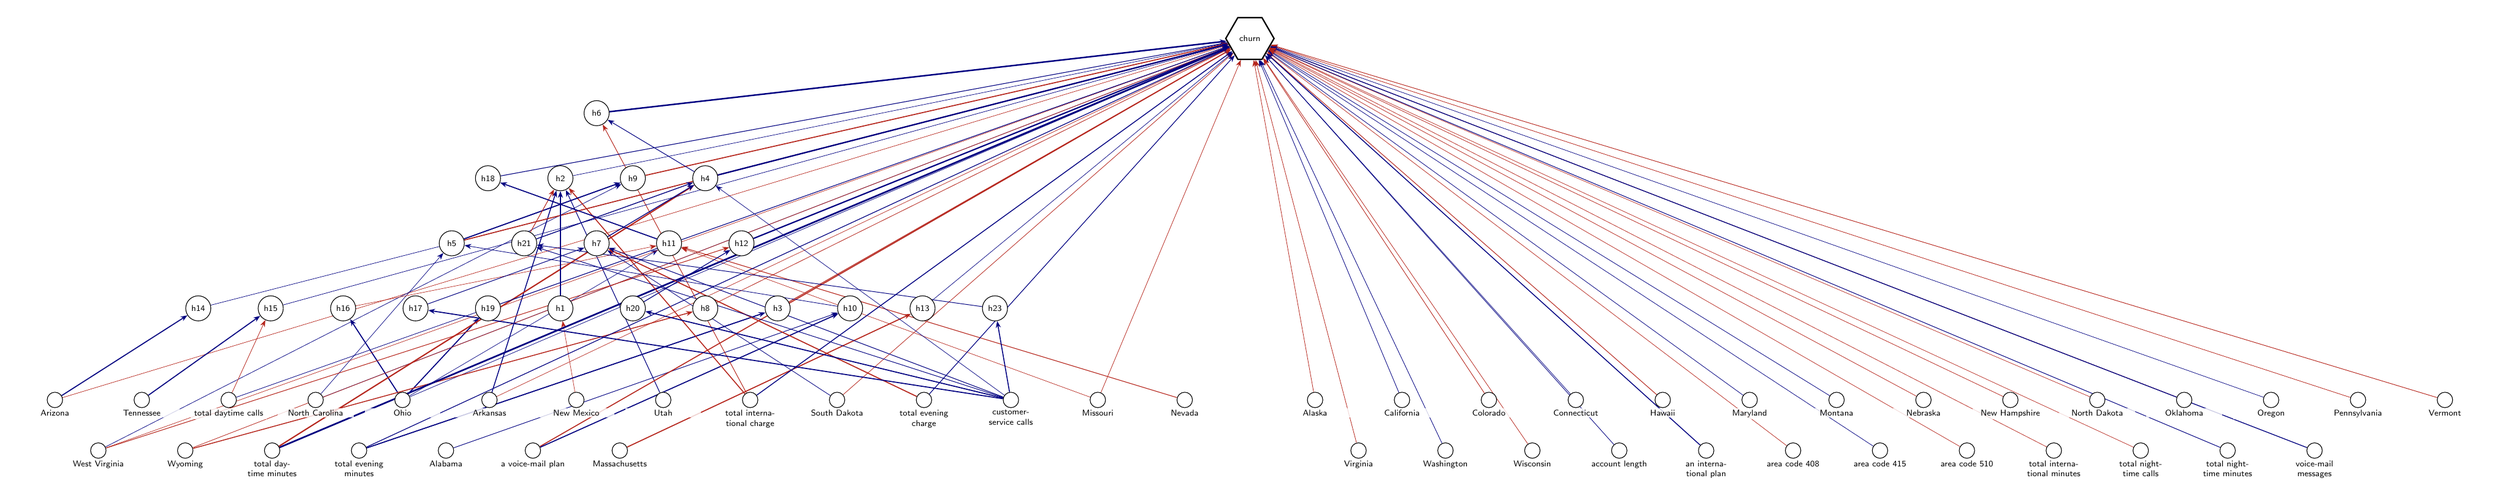
\begin{tikzpicture}[
  font=\sffamily\scriptsize, >={Stealth[length=1.4mm]},
  inp/.style={draw, circle, fill=white, minimum size=3.2mm, inner sep=0pt},
  hid/.style={draw, circle, fill=white, minimum size=5.2mm, inner sep=0.5pt, font=\sffamily\tiny},
  exitbox/.style={draw, thick, rectangle, fill=white, align=center, text width=17mm, minimum height=5mm, inner sep=1.5pt, font=\sffamily\tiny},
  sumbox/.style={draw, thick, dashed, rectangle, fill=white, align=center, text width=17mm, minimum height=5mm, inner sep=1.5pt, font=\sffamily\tiny},
  outp/.style={draw, thick, regular polygon, regular polygon sides=6, fill=white, minimum size=10mm, inner sep=0pt, font=\sffamily\tiny, align=center},
  stub/.style={draw, dashed, rounded corners=2pt, fill=white, align=center, inner sep=2pt, font=\sffamily\tiny, text width=15mm},
  inlab/.style={font=\sffamily\tiny, align=center, text width=15mm, inner sep=1pt, fill=white, fill opacity=0.8, text opacity=1},
  wpos/.style={draw=NavyBlue}, wneg/.style={draw=BrickRed}, wagg/.style={draw=black!45, line width=1.2pt},
  wmix/.style={draw=Plum},
]
\node[inp] (ninxxstatex0) at (26.1,0.0) {};
\path (ninxxstatex0.south) node[inlab, anchor=north] (labninxxstatex0) {Alaska};
\node[inp] (ninxxstatex19) at (11.7,-1.05) {};
\path (ninxxstatex19.south) node[inlab, anchor=north] (labninxxstatex19) {Massachusetts};
\node[inp] (ninxxstatex2) at (9.0,0.0) {};
\path (ninxxstatex2.south) node[inlab, anchor=north] (labninxxstatex2) {Arkansas};
\node[inp] (ninxxstatex20) at (35.1,0.0) {};
\path (ninxxstatex20.south) node[inlab, anchor=north] (labninxxstatex20) {Maryland};
\node[inp] (ninxxstatex24) at (21.6,0.0) {};
\path (ninxxstatex24.south) node[inlab, anchor=north] (labninxxstatex24) {Missouri};
\node[inp] (ninxxstatex1) at (8.1,-1.05) {};
\path (ninxxstatex1.south) node[inlab, anchor=north] (labninxxstatex1) {Alabama};
\node[inp] (ninxxstatex26) at (36.9,0.0) {};
\path (ninxxstatex26.south) node[inlab, anchor=north] (labninxxstatex26) {Montana};
\node[inp] (ninxxstatex27) at (5.4,0.0) {};
\path (ninxxstatex27.south) node[inlab, anchor=north] (labninxxstatex27) {North Carolina};
\node[inp] (ninxxstatex28) at (42.3,0.0) {};
\path (ninxxstatex28.south) node[inlab, anchor=north] (labninxxstatex28) {North Dakota};
\node[inp] (ninxxstatex29) at (38.7,0.0) {};
\path (ninxxstatex29.south) node[inlab, anchor=north] (labninxxstatex29) {Nebraska};
\node[inp] (ninxxstatex3) at (0.0,0.0) {};
\path (ninxxstatex3.south) node[inlab, anchor=north] (labninxxstatex3) {Arizona};
\node[inp] (ninxxstatex30) at (40.5,0.0) {};
\path (ninxxstatex30.south) node[inlab, anchor=north] (labninxxstatex30) {New Hampshire};
\node[inp] (ninxxstatex32) at (10.8,0.0) {};
\path (ninxxstatex32.south) node[inlab, anchor=north] (labninxxstatex32) {New Mexico};
\node[inp] (ninxxstatex33) at (23.4,0.0) {};
\path (ninxxstatex33.south) node[inlab, anchor=north] (labninxxstatex33) {Nevada};
\node[inp] (ninxxstatex35) at (7.2,0.0) {};
\path (ninxxstatex35.south) node[inlab, anchor=north] (labninxxstatex35) {Ohio};
\node[inp] (ninxxstatex36) at (44.1,0.0) {};
\path (ninxxstatex36.south) node[inlab, anchor=north] (labninxxstatex36) {Oklahoma};
\node[inp] (ninxxstatex37) at (45.9,0.0) {};
\path (ninxxstatex37.south) node[inlab, anchor=north] (labninxxstatex37) {Oregon};
\node[inp] (ninxxstatex38) at (47.7,0.0) {};
\path (ninxxstatex38.south) node[inlab, anchor=north] (labninxxstatex38) {Pennsylvania};
\node[inp] (ninxxstatex4) at (27.9,0.0) {};
\path (ninxxstatex4.south) node[inlab, anchor=north] (labninxxstatex4) {California};
\node[inp] (ninxxstatex41) at (16.2,0.0) {};
\path (ninxxstatex41.south) node[inlab, anchor=north] (labninxxstatex41) {South Dakota};
\node[inp] (ninxxstatex42) at (1.8,0.0) {};
\path (ninxxstatex42.south) node[inlab, anchor=north] (labninxxstatex42) {Tennessee};
\node[inp] (ninxxstatex11) at (33.3,0.0) {};
\path (ninxxstatex11.south) node[inlab, anchor=north] (labninxxstatex11) {Hawaii};
\node[inp] (ninxxstatex44) at (12.6,0.0) {};
\path (ninxxstatex44.south) node[inlab, anchor=north] (labninxxstatex44) {Utah};
\node[inp] (ninxxstatex45) at (27.0,-1.05) {};
\path (ninxxstatex45.south) node[inlab, anchor=north] (labninxxstatex45) {Virginia};
\node[inp] (ninxxstatex46) at (49.5,0.0) {};
\path (ninxxstatex46.south) node[inlab, anchor=north] (labninxxstatex46) {Vermont};
\node[inp] (ninxxstatex47) at (28.8,-1.05) {};
\path (ninxxstatex47.south) node[inlab, anchor=north] (labninxxstatex47) {Washington};
\node[inp] (ninxxstatex48) at (30.6,-1.05) {};
\path (ninxxstatex48.south) node[inlab, anchor=north] (labninxxstatex48) {Wisconsin};
\node[inp] (ninxxstatex49) at (0.9,-1.05) {};
\path (ninxxstatex49.south) node[inlab, anchor=north] (labninxxstatex49) {West Virginia};
\node[inp] (ninxxstatex5) at (29.7,0.0) {};
\path (ninxxstatex5.south) node[inlab, anchor=north] (labninxxstatex5) {Colorado};
\node[inp] (ninxxstatex50) at (2.7,-1.05) {};
\path (ninxxstatex50.south) node[inlab, anchor=north] (labninxxstatex50) {Wyoming};
\node[inp] (ninxxstatex6) at (31.5,0.0) {};
\path (ninxxstatex6.south) node[inlab, anchor=north] (labninxxstatex6) {Connecticut};
\node[inp] (ninxxaccountxlength) at (32.4,-1.05) {};
\path (ninxxaccountxlength.south) node[inlab, anchor=north] (labninxxaccountxlength) {account length};
\node[inp] (ninxxareaxcodex408) at (36.0,-1.05) {};
\path (ninxxareaxcodex408.south) node[inlab, anchor=north] (labninxxareaxcodex408) {area code 408};
\node[inp] (ninxxareaxcodex415) at (37.8,-1.05) {};
\path (ninxxareaxcodex415.south) node[inlab, anchor=north] (labninxxareaxcodex415) {area code 415};
\node[inp] (ninxxareaxcodex510) at (39.6,-1.05) {};
\path (ninxxareaxcodex510.south) node[inlab, anchor=north] (labninxxareaxcodex510) {area code 510};
\node[inp] (ninxxinternationalxplan) at (34.2,-1.05) {};
\path (ninxxinternationalxplan.south) node[inlab, anchor=north] (labninxxinternationalxplan) {an international plan};
\node[inp] (ninxxvoicexmailxplan) at (9.9,-1.05) {};
\path (ninxxvoicexmailxplan.south) node[inlab, anchor=north] (labninxxvoicexmailxplan) {a voice-mail plan};
\node[inp] (ninxxnumberxvmailxmessages) at (46.8,-1.05) {};
\path (ninxxnumberxvmailxmessages.south) node[inlab, anchor=north] (labninxxnumberxvmailxmessages) {voice-mail messages};
\node[inp] (ninxxtotalxdayxminutes) at (4.5,-1.05) {};
\path (ninxxtotalxdayxminutes.south) node[inlab, anchor=north] (labninxxtotalxdayxminutes) {total daytime minutes};
\node[inp] (ninxxtotalxdayxcalls) at (3.6,0.0) {};
\path (ninxxtotalxdayxcalls.south) node[inlab, anchor=north] (labninxxtotalxdayxcalls) {total daytime calls};
\node[inp] (ninxxtotalxevexminutes) at (6.3,-1.05) {};
\path (ninxxtotalxevexminutes.south) node[inlab, anchor=north] (labninxxtotalxevexminutes) {total evening minutes};
\node[inp] (ninxxtotalxevexcharge) at (18.0,0.0) {};
\path (ninxxtotalxevexcharge.south) node[inlab, anchor=north] (labninxxtotalxevexcharge) {total evening charge};
\node[inp] (ninxxtotalxnightxminutes) at (45.0,-1.05) {};
\path (ninxxtotalxnightxminutes.south) node[inlab, anchor=north] (labninxxtotalxnightxminutes) {total night-time minutes};
\node[inp] (ninxxtotalxnightxcalls) at (43.2,-1.05) {};
\path (ninxxtotalxnightxcalls.south) node[inlab, anchor=north] (labninxxtotalxnightxcalls) {total night-time calls};
\node[inp] (ninxxtotalxintlxminutes) at (41.4,-1.05) {};
\path (ninxxtotalxintlxminutes.south) node[inlab, anchor=north] (labninxxtotalxintlxminutes) {total international minutes};
\node[inp] (ninxxtotalxintlxcharge) at (14.4,0.0) {};
\path (ninxxtotalxintlxcharge.south) node[inlab, anchor=north] (labninxxtotalxintlxcharge) {total international charge};
\node[inp] (ninxxnumberxcustomerxservicexcalls) at (19.8,0.0) {};
\path (ninxxnumberxcustomerxservicexcalls.south) node[inlab, anchor=north] (labninxxnumberxcustomerxservicexcalls) {customer-service calls};
\node[outp] (n0) at (24.75,7.5) {churn};
\node[hid] (n10249) at (2.97,1.9) {h14};
\node[hid] (n1133) at (8.22,3.25) {h5};
\node[hid] (n11427) at (4.47,1.9) {h15};
\node[hid] (n11951) at (5.97,1.9) {h16};
\node[hid] (n1264) at (11.22,5.95) {h6};
\node[hid] (n12926) at (7.47,1.9) {h17};
\node[hid] (n13827) at (8.97,4.6) {h18};
\node[hid] (n14942) at (8.97,1.9) {h19};
\node[hid] (n161) at (10.47,1.9) {h1};
\node[hid] (n17032) at (11.97,1.9) {h20};
\node[hid] (n252) at (10.47,4.6) {h2};
\node[hid] (n2627) at (9.72,3.25) {h21};
\node[hid] (n2796) at (11.22,3.25) {h7};
\node[hid] (n3861) at (13.47,1.9) {h8};
\node[hid] (n4051) at (11.97,4.6) {h9};
\node[hid] (n476) at (14.97,1.9) {h3};
\node[hid] (n5577) at (16.47,1.9) {h10};
\node[hid] (n6730) at (12.72,3.25) {h11};
\node[hid] (n7208) at (14.22,3.25) {h12};
\node[hid] (n807) at (13.47,4.6) {h4};
\node[hid] (n8896) at (17.97,1.9) {h13};
\node[hid] (n9555) at (19.47,1.9) {h23};
\begin{scope}[on background layer]
\draw[->, wneg, line width=0.29pt] (ninxxstatex0) -- (n0);
\draw[->, wneg, line width=0.60pt] (ninxxstatex19) -- (n8896);
\draw[->, wneg, line width=0.25pt] (ninxxstatex2) -- (n0);
\draw[->, wpos, line width=0.52pt] (ninxxstatex2) -- (n252);
\draw[->, wpos, line width=0.28pt] (ninxxstatex20) -- (n0);
\draw[->, wneg, line width=0.28pt] (ninxxstatex24) -- (n0);
\draw[->, wneg, line width=0.25pt] (ninxxstatex24) -- (n6730);
\draw[->, wpos, line width=0.34pt] (ninxxstatex1) -- (n5577);
\draw[->, wpos, line width=0.28pt] (ninxxstatex26) -- (n0);
\draw[->, wpos, line width=0.26pt] (ninxxstatex27) -- (n0);
\draw[->, wpos, line width=0.26pt] (ninxxstatex27) -- (n1133);
\draw[->, wneg, line width=0.25pt] (ninxxstatex28) -- (n0);
\draw[->, wneg, line width=0.27pt] (ninxxstatex29) -- (n0);
\draw[->, wneg, line width=0.26pt] (ninxxstatex3) -- (n0);
\draw[->, wpos, line width=0.60pt] (ninxxstatex3) -- (n10249);
\draw[->, wneg, line width=0.27pt] (ninxxstatex30) -- (n0);
\draw[->, wneg, line width=0.25pt] (ninxxstatex32) -- (n161);
\draw[->, wneg, line width=0.40pt] (ninxxstatex33) -- (n6730);
\draw[->, wpos, line width=0.26pt] (ninxxstatex35) -- (n0);
\draw[->, wpos, line width=0.60pt] (ninxxstatex35) -- (n11951);
\draw[->, wpos, line width=0.60pt] (ninxxstatex35) -- (n14942);
\draw[->, wpos, line width=0.25pt] (ninxxstatex35) -- (n6730);
\draw[->, wneg, line width=0.26pt] (ninxxstatex36) -- (n0);
\draw[->, wpos, line width=0.26pt] (ninxxstatex37) -- (n0);
\draw[->, wneg, line width=0.29pt] (ninxxstatex38) -- (n0);
\draw[->, wpos, line width=0.30pt] (ninxxstatex4) -- (n0);
\draw[->, wneg, line width=0.29pt] (ninxxstatex41) -- (n0);
\draw[->, wpos, line width=0.30pt] (ninxxstatex41) -- (n2796);
\draw[->, wpos, line width=0.60pt] (ninxxstatex42) -- (n11427);
\draw[->, wneg, line width=0.36pt] (ninxxstatex11) -- (n0);
\draw[->, wpos, line width=0.40pt] (ninxxstatex44) -- (n252);
\draw[->, wneg, line width=0.29pt] (ninxxstatex45) -- (n0);
\draw[->, wneg, line width=0.34pt] (ninxxstatex46) -- (n0);
\draw[->, wpos, line width=0.30pt] (ninxxstatex47) -- (n0);
\draw[->, wneg, line width=0.28pt] (ninxxstatex48) -- (n0);
\draw[->, wneg, line width=0.25pt] (ninxxstatex49) -- (n0);
\draw[->, wpos, line width=0.27pt] (ninxxstatex49) -- (n4051);
\draw[->, wneg, line width=0.38pt] (ninxxstatex49) -- (n7208);
\draw[->, wneg, line width=0.32pt] (ninxxstatex5) -- (n0);
\draw[->, wneg, line width=0.29pt] (ninxxstatex50) -- (n0);
\draw[->, wneg, line width=0.52pt] (ninxxstatex50) -- (n3861);
\draw[->, wpos, line width=0.26pt] (ninxxstatex6) -- (n0);
\draw[->, wpos, line width=0.30pt] (ninxxaccountxlength) -- (n0);
\draw[->, wneg, line width=0.26pt] (ninxxareaxcodex408) -- (n0);
\draw[->, wpos, line width=0.27pt] (ninxxareaxcodex415) -- (n0);
\draw[->, wneg, line width=0.26pt] (ninxxareaxcodex510) -- (n0);
\draw[->, wpos, line width=0.51pt] (ninxxinternationalxplan) -- (n0);
\draw[->, wneg, line width=0.56pt] (ninxxvoicexmailxplan) -- (n0);
\draw[->, wpos, line width=0.60pt] (ninxxvoicexmailxplan) -- (n5577);
\draw[->, wpos, line width=0.47pt] (ninxxnumberxvmailxmessages) -- (n0);
\draw[->, wpos, line width=0.96pt] (ninxxtotalxdayxminutes) -- (n0);
\draw[->, wneg, line width=0.74pt] (ninxxtotalxdayxminutes) -- (n807);
\draw[->, wpos, line width=0.29pt] (ninxxtotalxdayxcalls) -- (n0);
\draw[->, wneg, line width=0.29pt] (ninxxtotalxdayxcalls) -- (n11427);
\draw[->, wpos, line width=0.43pt] (ninxxtotalxevexminutes) -- (n0);
\draw[->, wpos, line width=0.63pt] (ninxxtotalxevexminutes) -- (n476);
\draw[->, wpos, line width=0.41pt] (ninxxtotalxevexcharge) -- (n0);
\draw[->, wneg, line width=0.60pt] (ninxxtotalxevexcharge) -- (n2796);
\draw[->, wpos, line width=0.36pt] (ninxxtotalxnightxminutes) -- (n0);
\draw[->, wneg, line width=0.25pt] (ninxxtotalxnightxcalls) -- (n0);
\draw[->, wneg, line width=0.26pt] (ninxxtotalxintlxminutes) -- (n0);
\draw[->, wpos, line width=0.50pt] (ninxxtotalxintlxcharge) -- (n0);
\draw[->, wneg, line width=0.36pt] (ninxxtotalxintlxcharge) -- (n1264);
\draw[->, wneg, line width=0.55pt] (ninxxtotalxintlxcharge) -- (n252);
\draw[->, wpos, line width=0.60pt] (ninxxnumberxcustomerxservicexcalls) -- (n12926);
\draw[->, wpos, line width=0.60pt] (ninxxnumberxcustomerxservicexcalls) -- (n17032);
\draw[->, wpos, line width=0.35pt] (ninxxnumberxcustomerxservicexcalls) -- (n2627);
\draw[->, wpos, line width=0.38pt] (ninxxnumberxcustomerxservicexcalls) -- (n2796);
\draw[->, wpos, line width=0.26pt] (ninxxnumberxcustomerxservicexcalls) -- (n807);
\draw[->, wpos, line width=0.55pt] (ninxxnumberxcustomerxservicexcalls) -- (n9555);
\draw[->, wpos, line width=0.26pt] (n10249) -- (n0);
\draw[->, wneg, line width=0.58pt] (n1133) -- (n0);
\draw[->, wpos, line width=0.65pt] (n1133) -- (n4051);
\draw[->, wpos, line width=0.27pt] (n11427) -- (n0);
\draw[->, wneg, line width=0.25pt] (n11951) -- (n6730);
\draw[->, wpos, line width=0.88pt] (n1264) -- (n0);
\draw[->, wpos, line width=0.37pt] (n12926) -- (n2796);
\draw[->, wpos, line width=0.40pt] (n13827) -- (n0);
\draw[->, wpos, line width=0.26pt] (n14942) -- (n0);
\draw[->, wpos, line width=0.53pt] (n161) -- (n252);
\draw[->, wpos, line width=0.44pt] (n17032) -- (n7208);
\draw[->, wpos, line width=0.26pt] (n252) -- (n0);
\draw[->, wneg, line width=0.38pt] (n2627) -- (n252);
\draw[->, wpos, line width=0.49pt] (n2627) -- (n807);
\draw[->, wpos, line width=0.47pt] (n2796) -- (n807);
\draw[->, wneg, line width=0.30pt] (n3861) -- (n0);
\draw[->, wneg, line width=0.60pt] (n4051) -- (n0);
\draw[->, wneg, line width=0.44pt] (n476) -- (n0);
\draw[->, wpos, line width=0.30pt] (n5577) -- (n1133);
\draw[->, wpos, line width=0.60pt] (n6730) -- (n13827);
\draw[->, wpos, line width=0.77pt] (n7208) -- (n0);
\draw[->, wpos, line width=0.81pt] (n807) -- (n0);
\draw[->, wpos, line width=0.38pt] (n807) -- (n1264);
\draw[->, wpos, line width=0.26pt] (n8896) -- (n0);
\draw[->, wpos, line width=0.36pt] (n9555) -- (n2627);
\end{scope}
\end{tikzpicture}}%
\caption{The network as trained, before any explanation, in full. Blue: positive weight (raises the score); red: negative weight (lowers it); thicker: larger weight. Orange outline and up arrow: raises the final prediction; teal and down arrow: lowers it; grey and double arrow: depends. Not used (no connection): Georgia, Iowa, Idaho, Illinois, Indiana, Kansas, Kentucky, Louisiana, Maine, Michigan, Minnesota, Mississippi, New Jersey, New York, Rhode Island, South Carolina, Texas, Washington DC, Delaware, Florida, total daytime charge, total evening calls, total night-time charge, total international calls.}
\label{fig:churn100s2c1:raw}
\end{figure}
\end{landscape}
\end{drafted}
\clearpage
\end{document}
